\documentclass[twoside]{book}

% Packages required by doxygen
\usepackage{fixltx2e}
\usepackage{calc}
\usepackage{doxygen}
\usepackage[export]{adjustbox} % also loads graphicx
\usepackage{graphicx}
\usepackage[utf8]{inputenc}
\usepackage{makeidx}
\usepackage{multicol}
\usepackage{multirow}
\PassOptionsToPackage{warn}{textcomp}
\usepackage{textcomp}
\usepackage[nointegrals]{wasysym}
\usepackage[table]{xcolor}

% Font selection
\usepackage[T1]{fontenc}
\usepackage[scaled=.90]{helvet}
\usepackage{courier}
\usepackage{amssymb}
\usepackage{sectsty}
\renewcommand{\familydefault}{\sfdefault}
\allsectionsfont{%
  \fontseries{bc}\selectfont%
  \color{darkgray}%
}
\renewcommand{\DoxyLabelFont}{%
  \fontseries{bc}\selectfont%
  \color{darkgray}%
}
\newcommand{\+}{\discretionary{\mbox{\scriptsize$\hookleftarrow$}}{}{}}

% Page & text layout
\usepackage{geometry}
\geometry{%
  a4paper,%
  top=2.5cm,%
  bottom=2.5cm,%
  left=2.5cm,%
  right=2.5cm%
}
\tolerance=750
\hfuzz=15pt
\hbadness=750
\setlength{\emergencystretch}{15pt}
\setlength{\parindent}{0cm}
\setlength{\parskip}{3ex plus 2ex minus 2ex}
\makeatletter
\renewcommand{\paragraph}{%
  \@startsection{paragraph}{4}{0ex}{-1.0ex}{1.0ex}{%
    \normalfont\normalsize\bfseries\SS@parafont%
  }%
}
\renewcommand{\subparagraph}{%
  \@startsection{subparagraph}{5}{0ex}{-1.0ex}{1.0ex}{%
    \normalfont\normalsize\bfseries\SS@subparafont%
  }%
}
\makeatother

% Headers & footers
\usepackage{fancyhdr}
\pagestyle{fancyplain}
\fancyhead[LE]{\fancyplain{}{\bfseries\thepage}}
\fancyhead[CE]{\fancyplain{}{}}
\fancyhead[RE]{\fancyplain{}{\bfseries\leftmark}}
\fancyhead[LO]{\fancyplain{}{\bfseries\rightmark}}
\fancyhead[CO]{\fancyplain{}{}}
\fancyhead[RO]{\fancyplain{}{\bfseries\thepage}}
\fancyfoot[LE]{\fancyplain{}{}}
\fancyfoot[CE]{\fancyplain{}{}}
\fancyfoot[RE]{\fancyplain{}{\bfseries\scriptsize Generated by Doxygen }}
\fancyfoot[LO]{\fancyplain{}{\bfseries\scriptsize Generated by Doxygen }}
\fancyfoot[CO]{\fancyplain{}{}}
\fancyfoot[RO]{\fancyplain{}{}}
\renewcommand{\footrulewidth}{0.4pt}
\renewcommand{\chaptermark}[1]{%
  \markboth{#1}{}%
}
\renewcommand{\sectionmark}[1]{%
  \markright{\thesection\ #1}%
}

% Indices & bibliography
\usepackage{natbib}
\usepackage[titles]{tocloft}
\setcounter{tocdepth}{3}
\setcounter{secnumdepth}{5}
\makeindex

% Hyperlinks (required, but should be loaded last)
\usepackage{ifpdf}
\ifpdf
  \usepackage[pdftex,pagebackref=true]{hyperref}
\else
  \usepackage[ps2pdf,pagebackref=true]{hyperref}
\fi
\hypersetup{%
  colorlinks=true,%
  linkcolor=blue,%
  citecolor=blue,%
  unicode%
}

% Custom commands
\newcommand{\clearemptydoublepage}{%
  \newpage{\pagestyle{empty}\cleardoublepage}%
}

\usepackage{caption}
\captionsetup{labelsep=space,justification=centering,font={bf},singlelinecheck=off,skip=4pt,position=top}

%===== C O N T E N T S =====

\begin{document}

% Titlepage & ToC
\hypersetup{pageanchor=false,
             bookmarksnumbered=true,
             pdfencoding=unicode
            }
\pagenumbering{alph}
\begin{titlepage}
\vspace*{7cm}
\begin{center}%
{\Large Dungeon\+Crawler \\[1ex]\large 0.\+1v }\\
\vspace*{1cm}
{\large Generated by Doxygen 1.8.13}\\
\end{center}
\end{titlepage}
\clearemptydoublepage
\pagenumbering{roman}
\tableofcontents
\clearemptydoublepage
\pagenumbering{arabic}
\hypersetup{pageanchor=true}

%--- Begin generated contents ---
\chapter{Hierarchical Index}
\section{Class Hierarchy}
This inheritance list is sorted roughly, but not completely, alphabetically\+:\begin{DoxyCompactList}
\item \contentsline{section}{Basic\+Arrow}{\pageref{class_basic_arrow}}{}
\item Mono\+Behaviour\begin{DoxyCompactList}
\item \contentsline{section}{Approach\+Circle\+Script}{\pageref{class_approach_circle_script}}{}
\item \contentsline{section}{Arrow}{\pageref{class_arrow}}{}
\begin{DoxyCompactList}
\item \contentsline{section}{Basic\+Arrow}{\pageref{class_basic_arrow}}{}
\item \contentsline{section}{Delayed}{\pageref{class_delayed}}{}
\item \contentsline{section}{Fast\+Arrow}{\pageref{class_fast_arrow}}{}
\end{DoxyCompactList}
\item \contentsline{section}{Camera\+Controller}{\pageref{class_camera_controller}}{}
\item \contentsline{section}{Game\+Controller}{\pageref{class_game_controller}}{}
\item \contentsline{section}{Item\+Spawner}{\pageref{class_item_spawner}}{}
\item \contentsline{section}{Load\+Scene\+On\+Click}{\pageref{class_load_scene_on_click}}{}
\item \contentsline{section}{Mob1\+Movement}{\pageref{class_mob1_movement}}{}
\item \contentsline{section}{Mob2\+Movement}{\pageref{class_mob2_movement}}{}
\item \contentsline{section}{Mob\+Health}{\pageref{class_mob_health}}{}
\item \contentsline{section}{Osu\+Circle}{\pageref{class_osu_circle}}{}
\item \contentsline{section}{Pause\+Menu}{\pageref{class_pause_menu}}{}
\item \contentsline{section}{Pickup}{\pageref{class_pickup}}{}
\item \contentsline{section}{Player}{\pageref{class_player}}{}
\item \contentsline{section}{Quit\+On\+Click}{\pageref{class_quit_on_click}}{}
\item \contentsline{section}{Scene\+Controller}{\pageref{class_scene_controller}}{}
\item \contentsline{section}{Select\+On\+Input}{\pageref{class_select_on_input}}{}
\item \contentsline{section}{Shooting\+Aim\+Line}{\pageref{class_shooting_aim_line}}{}
\item \contentsline{section}{Spawn\+Controller}{\pageref{class_spawn_controller}}{}
\item \contentsline{section}{Spawn\+Pickups}{\pageref{class_spawn_pickups}}{}
\item \contentsline{section}{Spell\+Controller}{\pageref{class_spell_controller}}{}
\item \contentsline{section}{U\+I\+Controller}{\pageref{class_u_i_controller}}{}
\end{DoxyCompactList}
\item \contentsline{section}{Spell}{\pageref{class_spell}}{}
\end{DoxyCompactList}

\chapter{Class Index}
\section{Class List}
Here are the classes, structs, unions and interfaces with brief descriptions\+:\begin{DoxyCompactList}
\item\contentsline{section}{\hyperlink{class_approach_circle_script}{Approach\+Circle\+Script} }{\pageref{class_approach_circle_script}}{}
\item\contentsline{section}{\hyperlink{class_arrow}{Arrow} }{\pageref{class_arrow}}{}
\item\contentsline{section}{\hyperlink{class_basic_arrow}{Basic\+Arrow} }{\pageref{class_basic_arrow}}{}
\item\contentsline{section}{\hyperlink{class_basic_arrow}{Basic\+Arrow} }{\pageref{class_basic_arrow}}{}
\item\contentsline{section}{\hyperlink{class_camera_controller}{Camera\+Controller} }{\pageref{class_camera_controller}}{}
\item\contentsline{section}{\hyperlink{class_delayed}{Delayed} }{\pageref{class_delayed}}{}
\item\contentsline{section}{\hyperlink{class_fast_arrow}{Fast\+Arrow} }{\pageref{class_fast_arrow}}{}
\item\contentsline{section}{\hyperlink{class_game_controller}{Game\+Controller} }{\pageref{class_game_controller}}{}
\item\contentsline{section}{\hyperlink{class_item_spawner}{Item\+Spawner} }{\pageref{class_item_spawner}}{}
\item\contentsline{section}{\hyperlink{class_load_scene_on_click}{Load\+Scene\+On\+Click} }{\pageref{class_load_scene_on_click}}{}
\item\contentsline{section}{\hyperlink{class_mob1_movement}{Mob1\+Movement} }{\pageref{class_mob1_movement}}{}
\item\contentsline{section}{\hyperlink{class_mob2_movement}{Mob2\+Movement} }{\pageref{class_mob2_movement}}{}
\item\contentsline{section}{\hyperlink{class_mob_health}{Mob\+Health} }{\pageref{class_mob_health}}{}
\item\contentsline{section}{\hyperlink{class_osu_circle}{Osu\+Circle} }{\pageref{class_osu_circle}}{}
\item\contentsline{section}{\hyperlink{class_pause_menu}{Pause\+Menu} }{\pageref{class_pause_menu}}{}
\item\contentsline{section}{\hyperlink{class_pickup}{Pickup} }{\pageref{class_pickup}}{}
\item\contentsline{section}{\hyperlink{class_player}{Player} }{\pageref{class_player}}{}
\item\contentsline{section}{\hyperlink{class_quit_on_click}{Quit\+On\+Click} }{\pageref{class_quit_on_click}}{}
\item\contentsline{section}{\hyperlink{class_scene_controller}{Scene\+Controller} }{\pageref{class_scene_controller}}{}
\item\contentsline{section}{\hyperlink{class_select_on_input}{Select\+On\+Input} }{\pageref{class_select_on_input}}{}
\item\contentsline{section}{\hyperlink{class_shooting_aim_line}{Shooting\+Aim\+Line} }{\pageref{class_shooting_aim_line}}{}
\item\contentsline{section}{\hyperlink{class_spawn_controller}{Spawn\+Controller} }{\pageref{class_spawn_controller}}{}
\item\contentsline{section}{\hyperlink{class_spawn_pickups}{Spawn\+Pickups} }{\pageref{class_spawn_pickups}}{}
\item\contentsline{section}{\hyperlink{class_spell}{Spell} }{\pageref{class_spell}}{}
\item\contentsline{section}{\hyperlink{class_spell_controller}{Spell\+Controller} }{\pageref{class_spell_controller}}{}
\item\contentsline{section}{\hyperlink{class_u_i_controller}{U\+I\+Controller} }{\pageref{class_u_i_controller}}{}
\end{DoxyCompactList}

\chapter{Class Documentation}
\hypertarget{class_approach_circle_script}{}\section{Approach\+Circle\+Script Class Reference}
\label{class_approach_circle_script}\index{Approach\+Circle\+Script@{Approach\+Circle\+Script}}
Inheritance diagram for Approach\+Circle\+Script\+:\begin{figure}[H]
\begin{center}
\leavevmode
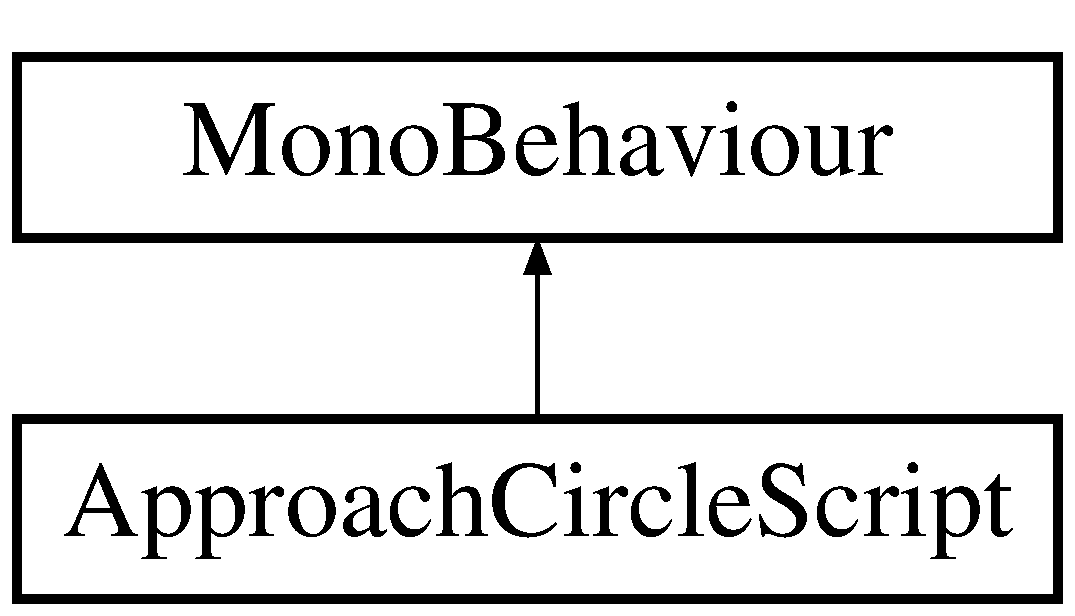
\includegraphics[height=2.000000cm]{class_approach_circle_script}
\end{center}
\end{figure}
\subsection*{Public Attributes}
\begin{DoxyCompactItemize}
\item 
\mbox{\Hypertarget{class_approach_circle_script_a49c18e052d6500a72c2be8995c3804d7}\label{class_approach_circle_script_a49c18e052d6500a72c2be8995c3804d7}} 
int \hyperlink{class_approach_circle_script_a49c18e052d6500a72c2be8995c3804d7}{segments}
\begin{DoxyCompactList}\small\item\em how many lines the circle is drawn with \end{DoxyCompactList}\item 
float \hyperlink{class_approach_circle_script_a5fe6dbba38877928ecd860156f44f68e}{xradius}
\begin{DoxyCompactList}\small\item\em Initial x\+Radius. \end{DoxyCompactList}\item 
float \hyperlink{class_approach_circle_script_a29314cfa6de27bac0b214a8be7834820}{yradius}
\begin{DoxyCompactList}\small\item\em Initial y\+Radius. \end{DoxyCompactList}\end{DoxyCompactItemize}
\subsection*{Private Member Functions}
\begin{DoxyCompactItemize}
\item 
void \hyperlink{class_approach_circle_script_a7fd2d08d8cf97264691ec5801f420dc4}{Start} ()
\item 
void \hyperlink{class_approach_circle_script_af02f62c7e58fbdfba5041a3f8b103faf}{Create\+Points} ()
\end{DoxyCompactItemize}
\subsection*{Private Attributes}
\begin{DoxyCompactItemize}
\item 
\mbox{\Hypertarget{class_approach_circle_script_a7a863d8532178a5657ee6a81f8d7f620}\label{class_approach_circle_script_a7a863d8532178a5657ee6a81f8d7f620}} 
Line\+Renderer \hyperlink{class_approach_circle_script_a7a863d8532178a5657ee6a81f8d7f620}{line}
\begin{DoxyCompactList}\small\item\em Line rendere of the approach circle. \end{DoxyCompactList}\end{DoxyCompactItemize}


\subsection{Detailed Description}
Script for handling how the circle around the osu circles interact 

\subsection{Member Function Documentation}
\mbox{\Hypertarget{class_approach_circle_script_af02f62c7e58fbdfba5041a3f8b103faf}\label{class_approach_circle_script_af02f62c7e58fbdfba5041a3f8b103faf}} 
\index{Approach\+Circle\+Script@{Approach\+Circle\+Script}!Create\+Points@{Create\+Points}}
\index{Create\+Points@{Create\+Points}!Approach\+Circle\+Script@{Approach\+Circle\+Script}}
\subsubsection{\texorpdfstring{Create\+Points()}{CreatePoints()}}
{\footnotesize\ttfamily void Approach\+Circle\+Script.\+Create\+Points (\begin{DoxyParamCaption}{ }\end{DoxyParamCaption})\hspace{0.3cm}{\ttfamily [private]}}

Handles points created \mbox{\Hypertarget{class_approach_circle_script_a7fd2d08d8cf97264691ec5801f420dc4}\label{class_approach_circle_script_a7fd2d08d8cf97264691ec5801f420dc4}} 
\index{Approach\+Circle\+Script@{Approach\+Circle\+Script}!Start@{Start}}
\index{Start@{Start}!Approach\+Circle\+Script@{Approach\+Circle\+Script}}
\subsubsection{\texorpdfstring{Start()}{Start()}}
{\footnotesize\ttfamily void Approach\+Circle\+Script.\+Start (\begin{DoxyParamCaption}{ }\end{DoxyParamCaption})\hspace{0.3cm}{\ttfamily [private]}}

sets Member values and creates Line\+Renderes from gameobject 

\subsection{Member Data Documentation}
\mbox{\Hypertarget{class_approach_circle_script_a5fe6dbba38877928ecd860156f44f68e}\label{class_approach_circle_script_a5fe6dbba38877928ecd860156f44f68e}} 
\index{Approach\+Circle\+Script@{Approach\+Circle\+Script}!xradius@{xradius}}
\index{xradius@{xradius}!Approach\+Circle\+Script@{Approach\+Circle\+Script}}
\subsubsection{\texorpdfstring{xradius}{xradius}}
{\footnotesize\ttfamily float Approach\+Circle\+Script.\+xradius}



Initial x\+Radius. 

\begin{DoxyNote}{Note}
should be the same as Y for a circle 
\end{DoxyNote}
\mbox{\Hypertarget{class_approach_circle_script_a29314cfa6de27bac0b214a8be7834820}\label{class_approach_circle_script_a29314cfa6de27bac0b214a8be7834820}} 
\index{Approach\+Circle\+Script@{Approach\+Circle\+Script}!yradius@{yradius}}
\index{yradius@{yradius}!Approach\+Circle\+Script@{Approach\+Circle\+Script}}
\subsubsection{\texorpdfstring{yradius}{yradius}}
{\footnotesize\ttfamily float Approach\+Circle\+Script.\+yradius}



Initial y\+Radius. 

\begin{DoxyNote}{Note}
should be the same as X for a circle 
\end{DoxyNote}


The documentation for this class was generated from the following file\+:\begin{DoxyCompactItemize}
\item 
Assets/\+Scripts/\+U\+I/\+Osu/Approach\+Circle\+Script.\+cs\end{DoxyCompactItemize}

\hypertarget{class_arrow}{}\section{Arrow Class Reference}
\label{class_arrow}\index{Arrow@{Arrow}}
Inheritance diagram for Arrow\+:\begin{figure}[H]
\begin{center}
\leavevmode
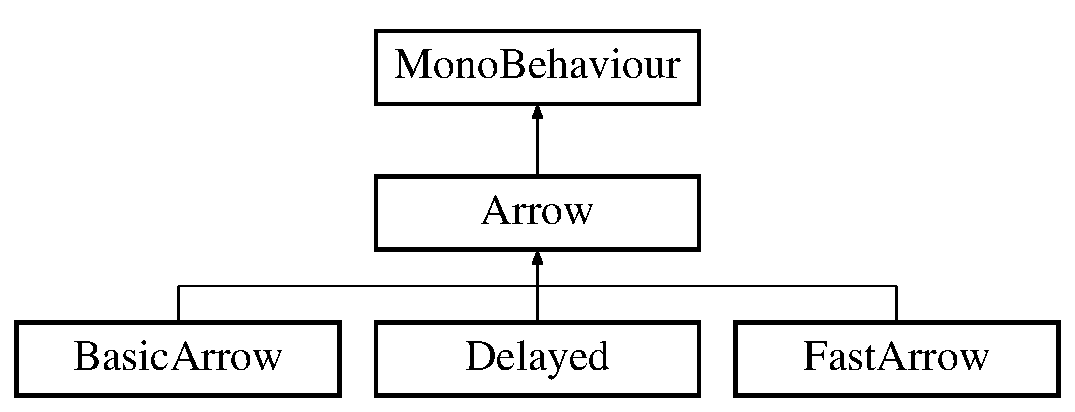
\includegraphics[height=3.000000cm]{class_arrow}
\end{center}
\end{figure}
\subsection*{Public Types}
\begin{DoxyCompactItemize}
\item 
\mbox{\Hypertarget{class_arrow_a6f10bb69bb3cb23483035a0eb1b286fa}\label{class_arrow_a6f10bb69bb3cb23483035a0eb1b286fa}} 
enum {\bfseries arrow\+Dmg\+Types} \{ {\bfseries basic} = 0, 
{\bfseries fire} = 1, 
{\bfseries ice} = 2, 
{\bfseries slow} = 3
 \}
\end{DoxyCompactItemize}
\subsection*{Public Member Functions}
\begin{DoxyCompactItemize}
\item 
void \hyperlink{class_arrow_a65ce0e1a14405dec237e13ee5631b07d}{Start} ()
\item 
void \hyperlink{class_arrow_aaf1023833f6420f4920d9013f9c46ef3}{Fixed\+Update} ()
\end{DoxyCompactItemize}
\subsection*{Public Attributes}
\begin{DoxyCompactItemize}
\item 
float \hyperlink{class_arrow_aae6ab7eee0fa3a72f17c4c46ce391e8a}{speed\+Mult}
\item 
float \hyperlink{class_arrow_a1ee7f10c0328ab7f8dccc8fcd061494b}{lifetime} = 2f
\item 
\mbox{\Hypertarget{class_arrow_a75efd0005fcd17e1425c4536b3c1c48b}\label{class_arrow_a75efd0005fcd17e1425c4536b3c1c48b}} 
Game\+Object {\bfseries model}
\item 
\hyperlink{class_player}{Player} \hyperlink{class_arrow_ac895e2c34f4eebe49198b1139b966541}{player} = null
\item 
\mbox{\Hypertarget{class_arrow_a312ad503e7ac9a4d4548c4a7ea096f75}\label{class_arrow_a312ad503e7ac9a4d4548c4a7ea096f75}} 
Audio\+Source {\bfseries source}
\item 
\mbox{\Hypertarget{class_arrow_ab10f23b78a724c0948d852e3fa11a2c1}\label{class_arrow_ab10f23b78a724c0948d852e3fa11a2c1}} 
arrow\+Dmg\+Types {\bfseries arrow\+Dmg\+Type} = arrow\+Dmg\+Types.\+basic
\end{DoxyCompactItemize}
\subsection*{Private Member Functions}
\begin{DoxyCompactItemize}
\item 
void \hyperlink{class_arrow_a186cf27bfba2bb5ce6b6427a44889858}{On\+Trigger\+Enter} (Collider col)
\item 
void \hyperlink{class_arrow_a87945ea993d85a6e1d1a59cd10b2358e}{Destroy\+Self} ()
\end{DoxyCompactItemize}
\subsection*{Private Attributes}
\begin{DoxyCompactItemize}
\item 
\mbox{\Hypertarget{class_arrow_a3fbdd74dc4c23d765744ece303a9599e}\label{class_arrow_a3fbdd74dc4c23d765744ece303a9599e}} 
\hyperlink{class_mob_health}{Mob\+Health} {\bfseries enemy}
\end{DoxyCompactItemize}


\subsection{Detailed Description}
Parent \hyperlink{class_arrow}{Arrow} class, which all arrows extend \begin{DoxyNote}{Note}
this class should never be instantiated on its own. 
\end{DoxyNote}


\subsection{Member Function Documentation}
\mbox{\Hypertarget{class_arrow_a87945ea993d85a6e1d1a59cd10b2358e}\label{class_arrow_a87945ea993d85a6e1d1a59cd10b2358e}} 
\index{Arrow@{Arrow}!Destroy\+Self@{Destroy\+Self}}
\index{Destroy\+Self@{Destroy\+Self}!Arrow@{Arrow}}
\subsubsection{\texorpdfstring{Destroy\+Self()}{DestroySelf()}}
{\footnotesize\ttfamily void Arrow.\+Destroy\+Self (\begin{DoxyParamCaption}{ }\end{DoxyParamCaption})\hspace{0.3cm}{\ttfamily [private]}}

Function called when \hyperlink{class_arrow}{Arrow} hits something. \textbackslash{} \begin{DoxyPostcond}{Postcondition}
Destorys \hyperlink{class_arrow}{Arrow} 
\end{DoxyPostcond}
\mbox{\Hypertarget{class_arrow_aaf1023833f6420f4920d9013f9c46ef3}\label{class_arrow_aaf1023833f6420f4920d9013f9c46ef3}} 
\index{Arrow@{Arrow}!Fixed\+Update@{Fixed\+Update}}
\index{Fixed\+Update@{Fixed\+Update}!Arrow@{Arrow}}
\subsubsection{\texorpdfstring{Fixed\+Update()}{FixedUpdate()}}
{\footnotesize\ttfamily void Arrow.\+Fixed\+Update (\begin{DoxyParamCaption}{ }\end{DoxyParamCaption})}

Defines movement for all arrows All arrows that extend \hyperlink{class_arrow}{Arrow} bust class this function at somepoint in their fixed\+Update(); \mbox{\Hypertarget{class_arrow_a186cf27bfba2bb5ce6b6427a44889858}\label{class_arrow_a186cf27bfba2bb5ce6b6427a44889858}} 
\index{Arrow@{Arrow}!On\+Trigger\+Enter@{On\+Trigger\+Enter}}
\index{On\+Trigger\+Enter@{On\+Trigger\+Enter}!Arrow@{Arrow}}
\subsubsection{\texorpdfstring{On\+Trigger\+Enter()}{OnTriggerEnter()}}
{\footnotesize\ttfamily void Arrow.\+On\+Trigger\+Enter (\begin{DoxyParamCaption}\item[{Collider}]{col }\end{DoxyParamCaption})\hspace{0.3cm}{\ttfamily [private]}}

Event handler for when arrow hits an object with a collider 
\begin{DoxyParams}{Parameters}
{\em col} & is the other object \\
\hline
\end{DoxyParams}
\mbox{\Hypertarget{class_arrow_a65ce0e1a14405dec237e13ee5631b07d}\label{class_arrow_a65ce0e1a14405dec237e13ee5631b07d}} 
\index{Arrow@{Arrow}!Start@{Start}}
\index{Start@{Start}!Arrow@{Arrow}}
\subsubsection{\texorpdfstring{Start()}{Start()}}
{\footnotesize\ttfamily void Arrow.\+Start (\begin{DoxyParamCaption}{ }\end{DoxyParamCaption})}

any arrow class that extends this, must class this function with Base\+Arrow = base.\+game\+Object.\+Get\+Component$<$\+Arrow$>$(); Base\+Arrow.\+Start(); 

\subsection{Member Data Documentation}
\mbox{\Hypertarget{class_arrow_a1ee7f10c0328ab7f8dccc8fcd061494b}\label{class_arrow_a1ee7f10c0328ab7f8dccc8fcd061494b}} 
\index{Arrow@{Arrow}!lifetime@{lifetime}}
\index{lifetime@{lifetime}!Arrow@{Arrow}}
\subsubsection{\texorpdfstring{lifetime}{lifetime}}
{\footnotesize\ttfamily float Arrow.\+lifetime = 2f}

Overall Lifetime of the arrow in seconds (To be extended in child class) \mbox{\Hypertarget{class_arrow_ac895e2c34f4eebe49198b1139b966541}\label{class_arrow_ac895e2c34f4eebe49198b1139b966541}} 
\index{Arrow@{Arrow}!player@{player}}
\index{player@{player}!Arrow@{Arrow}}
\subsubsection{\texorpdfstring{player}{player}}
{\footnotesize\ttfamily \hyperlink{class_player}{Player} Arrow.\+player = null}

Will be set in \hyperlink{class_arrow_a65ce0e1a14405dec237e13ee5631b07d}{Start()} function \mbox{\Hypertarget{class_arrow_aae6ab7eee0fa3a72f17c4c46ce391e8a}\label{class_arrow_aae6ab7eee0fa3a72f17c4c46ce391e8a}} 
\index{Arrow@{Arrow}!speed\+Mult@{speed\+Mult}}
\index{speed\+Mult@{speed\+Mult}!Arrow@{Arrow}}
\subsubsection{\texorpdfstring{speed\+Mult}{speedMult}}
{\footnotesize\ttfamily float Arrow.\+speed\+Mult}

Overall speed of the arrow (To be extended in child class) 

The documentation for this class was generated from the following file\+:\begin{DoxyCompactItemize}
\item 
Assets/\+Scripts/\+Arrows/Arrow.\+cs\end{DoxyCompactItemize}

\hypertarget{class_basic_arrow}{}\section{Basic\+Arrow Class Reference}
\label{class_basic_arrow}\index{Basic\+Arrow@{Basic\+Arrow}}
Inheritance diagram for Basic\+Arrow\+:\begin{figure}[H]
\begin{center}
\leavevmode
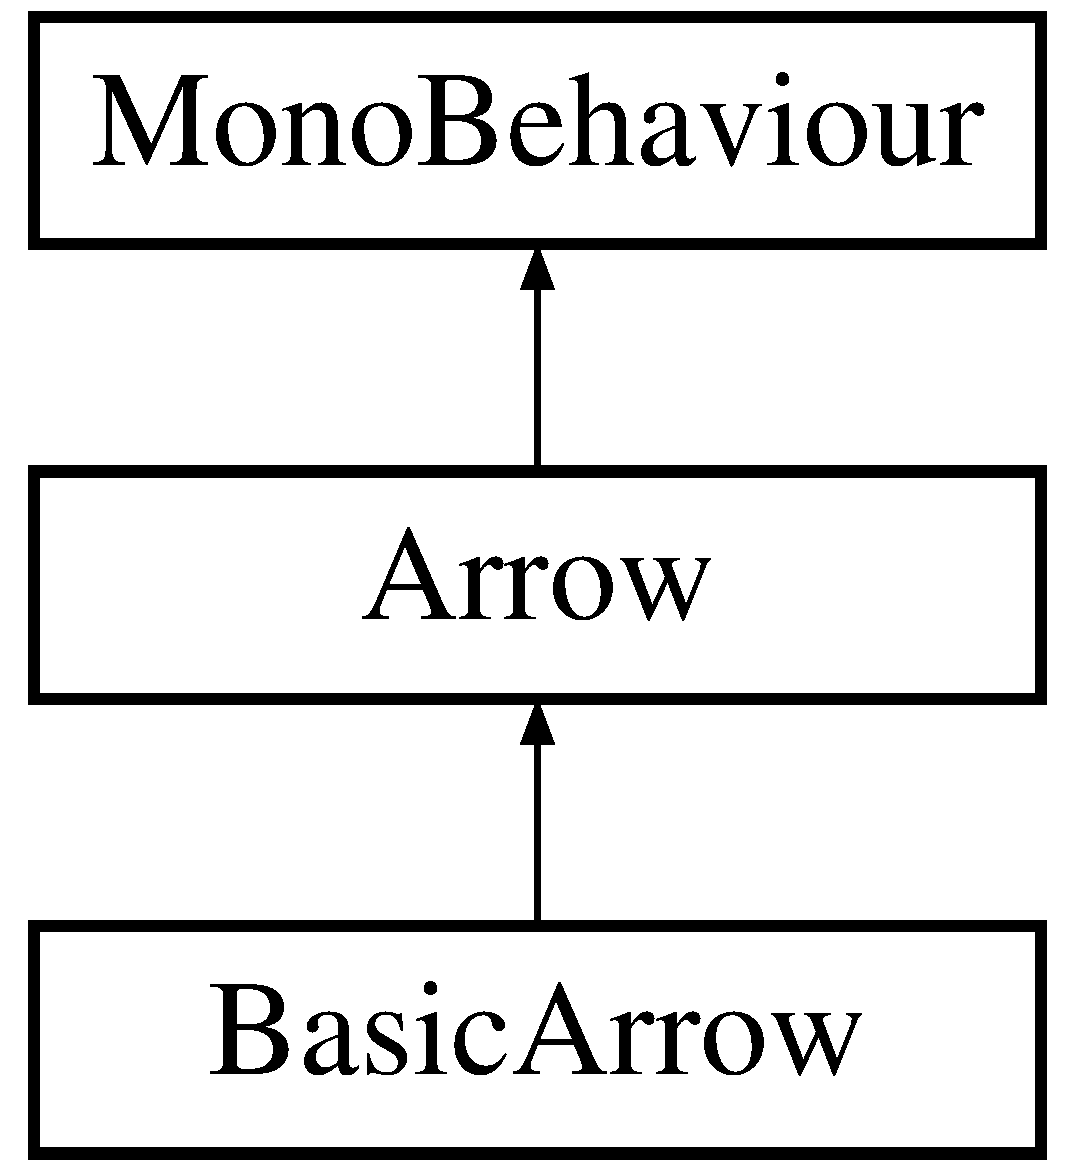
\includegraphics[height=3.000000cm]{class_basic_arrow}
\end{center}
\end{figure}
\subsection*{Private Member Functions}
\begin{DoxyCompactItemize}
\item 
new void \hyperlink{class_basic_arrow_a17d5a6491f2ce81238738282ad62d8ea}{Start} ()
\item 
\mbox{\Hypertarget{class_basic_arrow_a8167048ebf5b6c8302ea51ab0e44ec5f}\label{class_basic_arrow_a8167048ebf5b6c8302ea51ab0e44ec5f}} 
void {\bfseries Update} ()
\end{DoxyCompactItemize}
\subsection*{Private Attributes}
\begin{DoxyCompactItemize}
\item 
\mbox{\Hypertarget{class_basic_arrow_add301fff3d455823b42c2f870885b1f0}\label{class_basic_arrow_add301fff3d455823b42c2f870885b1f0}} 
\hyperlink{class_arrow}{Arrow} \hyperlink{class_basic_arrow_add301fff3d455823b42c2f870885b1f0}{Base\+Arrow}
\begin{DoxyCompactList}\small\item\em Base arrow component to get set in start() \end{DoxyCompactList}\end{DoxyCompactItemize}
\subsection*{Additional Inherited Members}


\subsection{Detailed Description}
Dictates which kind of arrow \textquotesingle{}type\textquotesingle{} it is. Some arrows are basic even though they aren\textquotesingle{}t just

Basic \hyperlink{class_arrow}{Arrow} class This is a default arrow that should be fired when nothing else is loaded/clicked on. \begin{DoxyNote}{Note}
Prefab class 
\end{DoxyNote}


\subsection{Member Function Documentation}
\mbox{\Hypertarget{class_basic_arrow_a17d5a6491f2ce81238738282ad62d8ea}\label{class_basic_arrow_a17d5a6491f2ce81238738282ad62d8ea}} 
\index{Basic\+Arrow@{Basic\+Arrow}!Start@{Start}}
\index{Start@{Start}!Basic\+Arrow@{Basic\+Arrow}}
\subsubsection{\texorpdfstring{Start()}{Start()}}
{\footnotesize\ttfamily new void Basic\+Arrow.\+Start (\begin{DoxyParamCaption}{ }\end{DoxyParamCaption})\hspace{0.3cm}{\ttfamily [private]}}

\begin{DoxyPostcond}{Postcondition}
calls Base\+Arrow.\+Start(), then the parent class handels everything else. 
\end{DoxyPostcond}
\begin{DoxyNote}{Note}
it appears that this needs to be called otherwise the object won\textquotesingle{}t instantiate it\textquotesingle{}s parent class 
\end{DoxyNote}


The documentation for this class was generated from the following files\+:\begin{DoxyCompactItemize}
\item 
Assets/\+Scripts/\+Arrows/Arrow.\+cs\item 
Assets/\+Scripts/\+Arrows/Basic\+Arrow.\+cs\end{DoxyCompactItemize}

\hypertarget{class_basic_arrow}{}\section{Basic\+Arrow Class Reference}
\label{class_basic_arrow}\index{Basic\+Arrow@{Basic\+Arrow}}
Inheritance diagram for Basic\+Arrow\+:\begin{figure}[H]
\begin{center}
\leavevmode
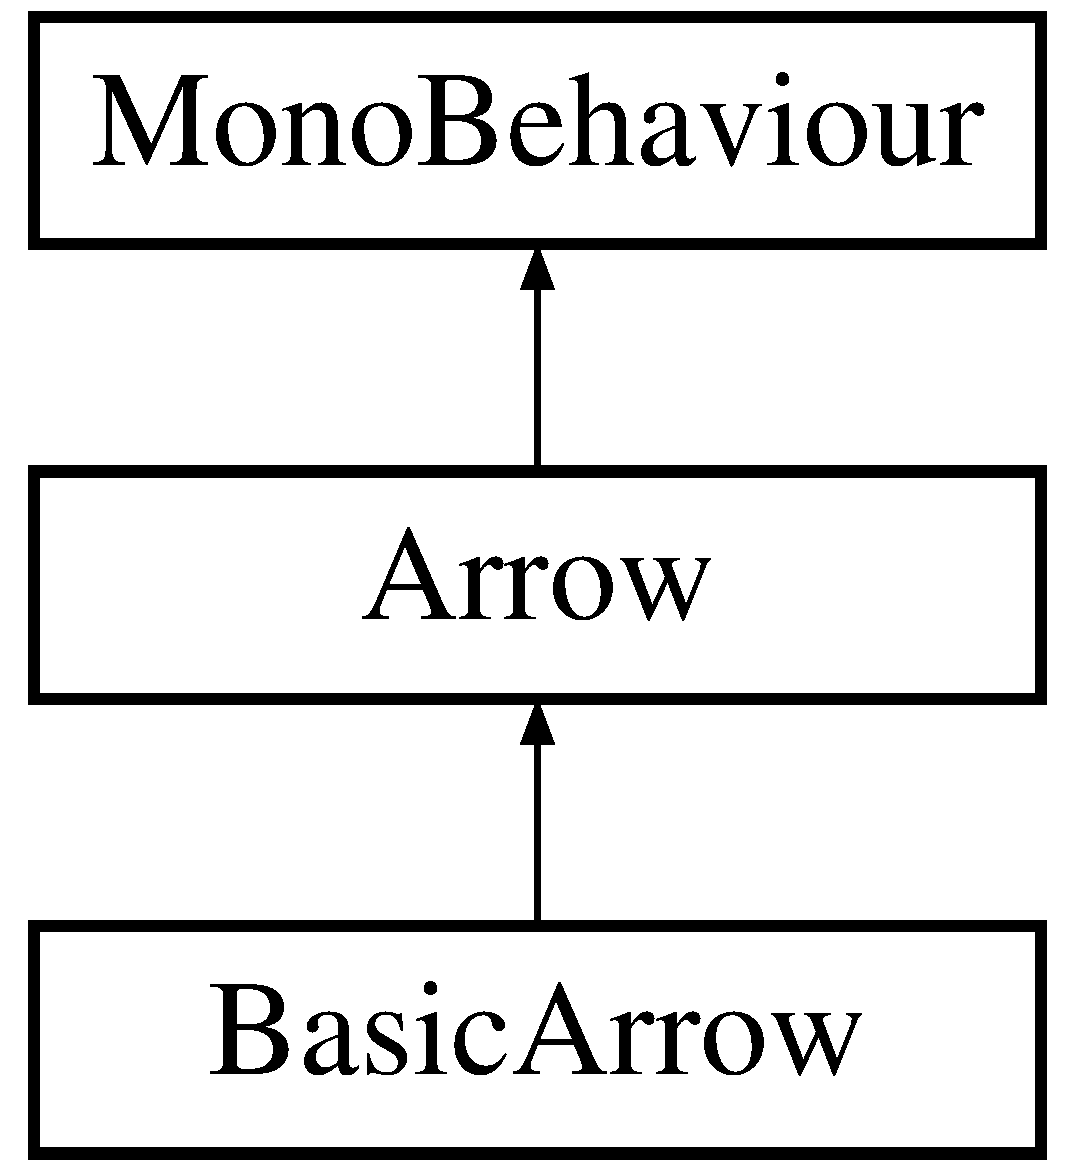
\includegraphics[height=3.000000cm]{class_basic_arrow}
\end{center}
\end{figure}
\subsection*{Private Member Functions}
\begin{DoxyCompactItemize}
\item 
new void \hyperlink{class_basic_arrow_a17d5a6491f2ce81238738282ad62d8ea}{Start} ()
\item 
\mbox{\Hypertarget{class_basic_arrow_a8167048ebf5b6c8302ea51ab0e44ec5f}\label{class_basic_arrow_a8167048ebf5b6c8302ea51ab0e44ec5f}} 
void {\bfseries Update} ()
\end{DoxyCompactItemize}
\subsection*{Private Attributes}
\begin{DoxyCompactItemize}
\item 
\mbox{\Hypertarget{class_basic_arrow_add301fff3d455823b42c2f870885b1f0}\label{class_basic_arrow_add301fff3d455823b42c2f870885b1f0}} 
\hyperlink{class_arrow}{Arrow} \hyperlink{class_basic_arrow_add301fff3d455823b42c2f870885b1f0}{Base\+Arrow}
\begin{DoxyCompactList}\small\item\em Base arrow component to get set in start() \end{DoxyCompactList}\end{DoxyCompactItemize}
\subsection*{Additional Inherited Members}


\subsection{Detailed Description}
Dictates which kind of arrow \textquotesingle{}type\textquotesingle{} it is. Some arrows are basic even though they aren\textquotesingle{}t just

Basic \hyperlink{class_arrow}{Arrow} class This is a default arrow that should be fired when nothing else is loaded/clicked on. \begin{DoxyNote}{Note}
Prefab class 
\end{DoxyNote}


\subsection{Member Function Documentation}
\mbox{\Hypertarget{class_basic_arrow_a17d5a6491f2ce81238738282ad62d8ea}\label{class_basic_arrow_a17d5a6491f2ce81238738282ad62d8ea}} 
\index{Basic\+Arrow@{Basic\+Arrow}!Start@{Start}}
\index{Start@{Start}!Basic\+Arrow@{Basic\+Arrow}}
\subsubsection{\texorpdfstring{Start()}{Start()}}
{\footnotesize\ttfamily new void Basic\+Arrow.\+Start (\begin{DoxyParamCaption}{ }\end{DoxyParamCaption})\hspace{0.3cm}{\ttfamily [private]}}

\begin{DoxyPostcond}{Postcondition}
calls Base\+Arrow.\+Start(), then the parent class handels everything else. 
\end{DoxyPostcond}
\begin{DoxyNote}{Note}
it appears that this needs to be called otherwise the object won\textquotesingle{}t instantiate it\textquotesingle{}s parent class 
\end{DoxyNote}


The documentation for this class was generated from the following files\+:\begin{DoxyCompactItemize}
\item 
Assets/\+Scripts/\+Arrows/Arrow.\+cs\item 
Assets/\+Scripts/\+Arrows/Basic\+Arrow.\+cs\end{DoxyCompactItemize}

\hypertarget{class_camera_controller}{}\section{Camera\+Controller Class Reference}
\label{class_camera_controller}\index{Camera\+Controller@{Camera\+Controller}}
Inheritance diagram for Camera\+Controller\+:\begin{figure}[H]
\begin{center}
\leavevmode
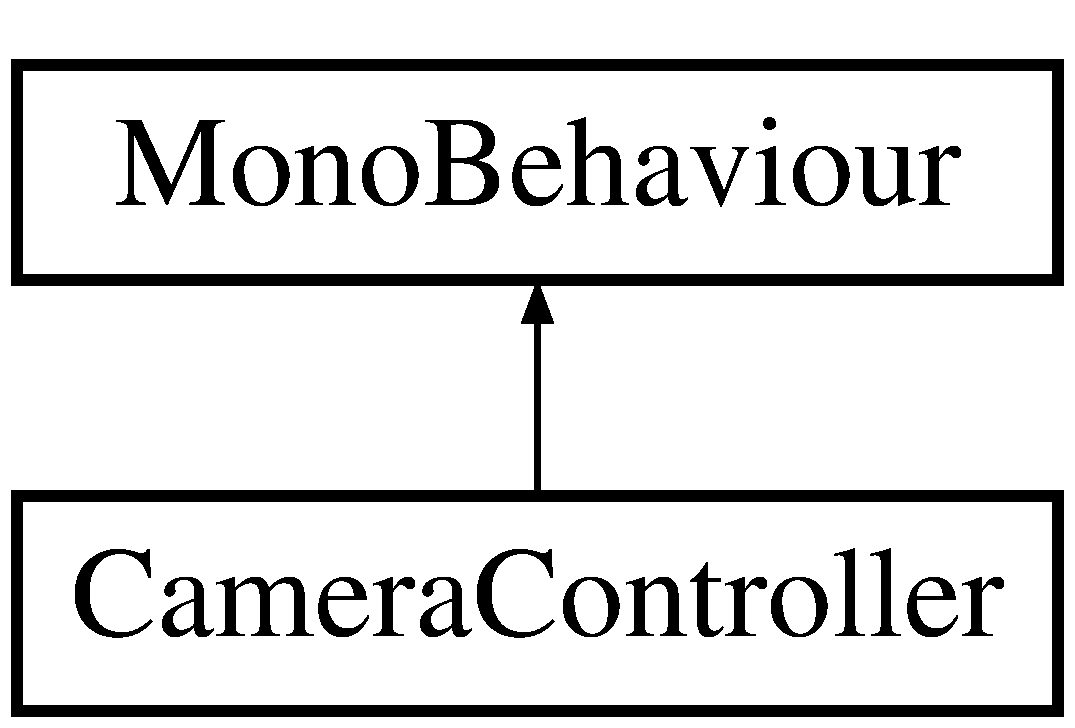
\includegraphics[height=2.000000cm]{class_camera_controller}
\end{center}
\end{figure}
\subsection*{Private Member Functions}
\begin{DoxyCompactItemize}
\item 
void \hyperlink{class_camera_controller_ad4a238c6f7db3ee003302a245d860860}{Start} ()
\item 
void \hyperlink{class_camera_controller_afcd241727886518c21b9609193e32d18}{Late\+Update} ()
\end{DoxyCompactItemize}
\subsection*{Private Attributes}
\begin{DoxyCompactItemize}
\item 
\mbox{\Hypertarget{class_camera_controller_aff80d2275dae360196361c39078bfda4}\label{class_camera_controller_aff80d2275dae360196361c39078bfda4}} 
Vector3 \hyperlink{class_camera_controller_aff80d2275dae360196361c39078bfda4}{offset}
\begin{DoxyCompactList}\small\item\em Offset of the world to camera position. \end{DoxyCompactList}\item 
\mbox{\Hypertarget{class_camera_controller_aae794ec2d17947f671ce0eaef9aac8b7}\label{class_camera_controller_aae794ec2d17947f671ce0eaef9aac8b7}} 
Game\+Object \hyperlink{class_camera_controller_aae794ec2d17947f671ce0eaef9aac8b7}{player}
\begin{DoxyCompactList}\small\item\em \hyperlink{class_player}{Player} Game\+Object to track movement. \end{DoxyCompactList}\end{DoxyCompactItemize}


\subsection{Detailed Description}
Class that manages the movement of the Camera 

\subsection{Member Function Documentation}
\mbox{\Hypertarget{class_camera_controller_afcd241727886518c21b9609193e32d18}\label{class_camera_controller_afcd241727886518c21b9609193e32d18}} 
\index{Camera\+Controller@{Camera\+Controller}!Late\+Update@{Late\+Update}}
\index{Late\+Update@{Late\+Update}!Camera\+Controller@{Camera\+Controller}}
\subsubsection{\texorpdfstring{Late\+Update()}{LateUpdate()}}
{\footnotesize\ttfamily void Camera\+Controller.\+Late\+Update (\begin{DoxyParamCaption}{ }\end{DoxyParamCaption})\hspace{0.3cm}{\ttfamily [private]}}

Updates the camera position to follow the player \begin{DoxyNote}{Note}
\hyperlink{class_camera_controller_afcd241727886518c21b9609193e32d18}{Late\+Update()} to avoid unexpected behaviors with other gameobject updates(). Last thing in the scene to update 
\end{DoxyNote}
\mbox{\Hypertarget{class_camera_controller_ad4a238c6f7db3ee003302a245d860860}\label{class_camera_controller_ad4a238c6f7db3ee003302a245d860860}} 
\index{Camera\+Controller@{Camera\+Controller}!Start@{Start}}
\index{Start@{Start}!Camera\+Controller@{Camera\+Controller}}
\subsubsection{\texorpdfstring{Start()}{Start()}}
{\footnotesize\ttfamily void Camera\+Controller.\+Start (\begin{DoxyParamCaption}{ }\end{DoxyParamCaption})\hspace{0.3cm}{\ttfamily [private]}}

\begin{DoxyPostcond}{Postcondition}
private members to appropriate objects 
\end{DoxyPostcond}


The documentation for this class was generated from the following file\+:\begin{DoxyCompactItemize}
\item 
Assets/\+Scripts/\+Controllers/Camera\+Controller.\+cs\end{DoxyCompactItemize}

\hypertarget{class_delayed}{}\section{Delayed Class Reference}
\label{class_delayed}\index{Delayed@{Delayed}}
Inheritance diagram for Delayed\+:\begin{figure}[H]
\begin{center}
\leavevmode
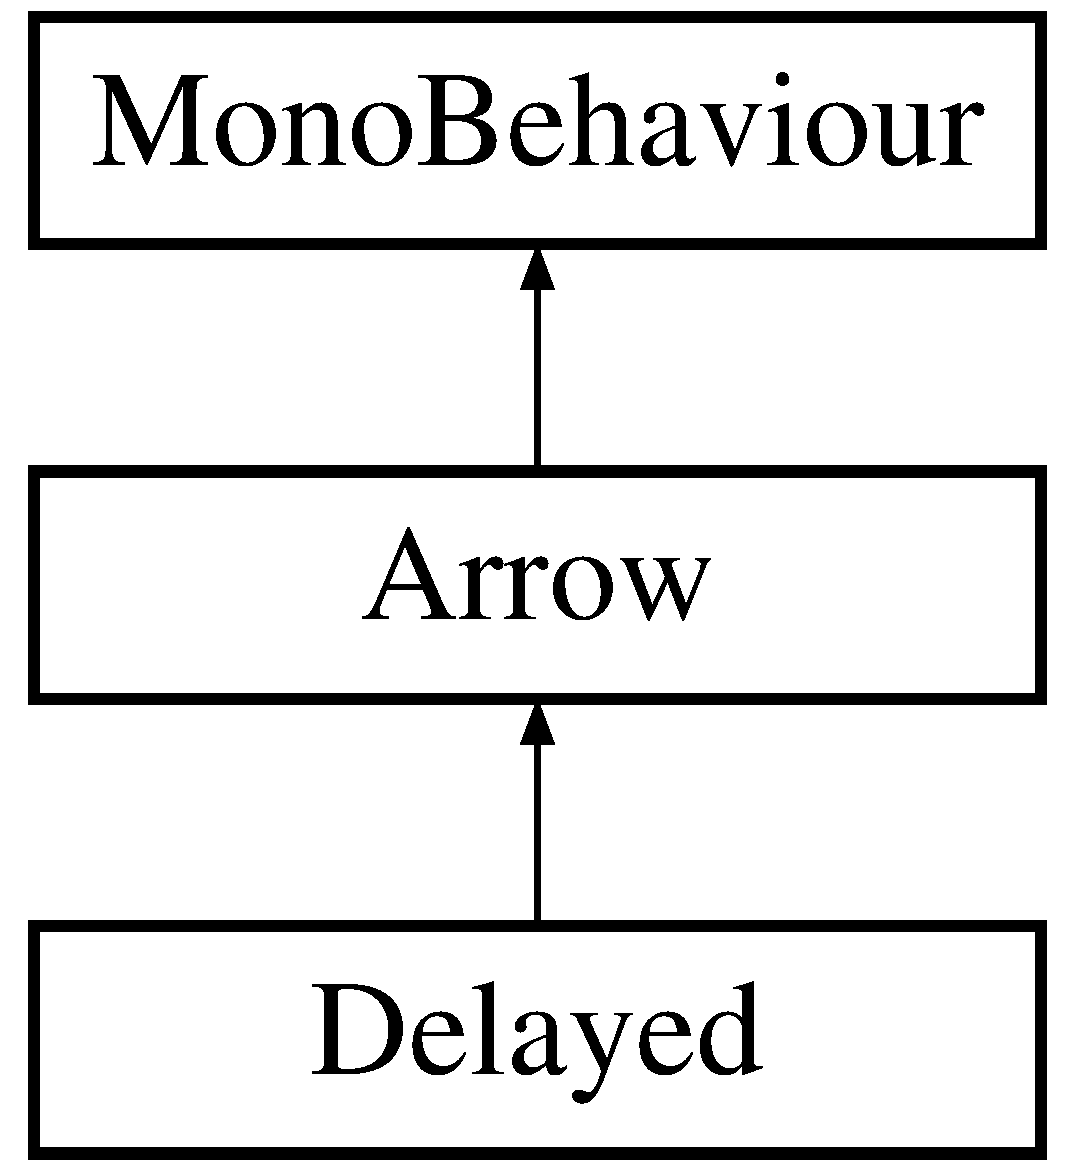
\includegraphics[height=3.000000cm]{class_delayed}
\end{center}
\end{figure}
\subsection*{Public Attributes}
\begin{DoxyCompactItemize}
\item 
\mbox{\Hypertarget{class_delayed_ace12fa36fce732dcb6302d3fc5a43a12}\label{class_delayed_ace12fa36fce732dcb6302d3fc5a43a12}} 
Game\+Object \hyperlink{class_delayed_ace12fa36fce732dcb6302d3fc5a43a12}{Basic\+Arrow}
\begin{DoxyCompactList}\small\item\em Gameobject to be instantiate. In this case the \hyperlink{class_basic_arrow}{Basic\+Arrow} prefab. \end{DoxyCompactList}\item 
\mbox{\Hypertarget{class_delayed_a2d248a33685341b8645c8060c6e291bd}\label{class_delayed_a2d248a33685341b8645c8060c6e291bd}} 
float \hyperlink{class_delayed_a2d248a33685341b8645c8060c6e291bd}{spawntimer}
\begin{DoxyCompactList}\small\item\em Set how long the spawning will continue for. \end{DoxyCompactList}\end{DoxyCompactItemize}
\subsection*{Private Member Functions}
\begin{DoxyCompactItemize}
\item 
new void \hyperlink{class_delayed_a680d8010c92af858e6d0ee4fe4711961}{Start} ()
\item 
new void \hyperlink{class_delayed_a2c17802ed1b249f91240a20a07ef1019}{Fixed\+Update} ()
\end{DoxyCompactItemize}
\subsection*{Private Attributes}
\begin{DoxyCompactItemize}
\item 
\mbox{\Hypertarget{class_delayed_a0acfe588c36cd67c143d8c293f32ff7e}\label{class_delayed_a0acfe588c36cd67c143d8c293f32ff7e}} 
\hyperlink{class_arrow}{Arrow} \hyperlink{class_delayed_a0acfe588c36cd67c143d8c293f32ff7e}{Base\+Arrow}
\begin{DoxyCompactList}\small\item\em Base\+Arrow Component. \end{DoxyCompactList}\item 
\mbox{\Hypertarget{class_delayed_a53603baf85cfda409690e85740cff1d6}\label{class_delayed_a53603baf85cfda409690e85740cff1d6}} 
float \hyperlink{class_delayed_a53603baf85cfda409690e85740cff1d6}{spawntime}
\begin{DoxyCompactList}\small\item\em float to keep track of current time in gameworld. \end{DoxyCompactList}\item 
\mbox{\Hypertarget{class_delayed_a7e66f6655bed06e61335d2de08327c66}\label{class_delayed_a7e66f6655bed06e61335d2de08327c66}} 
Vector3 \hyperlink{class_delayed_a7e66f6655bed06e61335d2de08327c66}{Initial\+Position}
\begin{DoxyCompactList}\small\item\em sets position to spawn new Basic\+Arrows \end{DoxyCompactList}\end{DoxyCompactItemize}
\subsection*{Additional Inherited Members}


\subsection{Detailed Description}
\hyperlink{class_delayed}{Delayed} arrow shoots one arrow, then spawns more basic arrows in the same direction for a set duration. \begin{DoxyNote}{Note}
Death of this arrow type is managed by the parent class 

Prefab class 
\end{DoxyNote}


\subsection{Member Function Documentation}
\mbox{\Hypertarget{class_delayed_a2c17802ed1b249f91240a20a07ef1019}\label{class_delayed_a2c17802ed1b249f91240a20a07ef1019}} 
\index{Delayed@{Delayed}!Fixed\+Update@{Fixed\+Update}}
\index{Fixed\+Update@{Fixed\+Update}!Delayed@{Delayed}}
\subsubsection{\texorpdfstring{Fixed\+Update()}{FixedUpdate()}}
{\footnotesize\ttfamily new void Delayed.\+Fixed\+Update (\begin{DoxyParamCaption}{ }\end{DoxyParamCaption})\hspace{0.3cm}{\ttfamily [private]}}

Calls base\+Arrow fixed\+Update() and then instantiates more arrows if Time.\+time $>$ spawntime \mbox{\Hypertarget{class_delayed_a680d8010c92af858e6d0ee4fe4711961}\label{class_delayed_a680d8010c92af858e6d0ee4fe4711961}} 
\index{Delayed@{Delayed}!Start@{Start}}
\index{Start@{Start}!Delayed@{Delayed}}
\subsubsection{\texorpdfstring{Start()}{Start()}}
{\footnotesize\ttfamily new void Delayed.\+Start (\begin{DoxyParamCaption}{ }\end{DoxyParamCaption})\hspace{0.3cm}{\ttfamily [private]}}

Sets spawntime of next basic arrow to Time.\+time + spawntimer. \begin{DoxyPostcond}{Postcondition}
a set object invisible object that spawns more basearrows. 
\end{DoxyPostcond}


The documentation for this class was generated from the following file\+:\begin{DoxyCompactItemize}
\item 
Assets/\+Scripts/\+Arrows/Delayed.\+cs\end{DoxyCompactItemize}

\hypertarget{class_fast_arrow}{}\section{Fast\+Arrow Class Reference}
\label{class_fast_arrow}\index{Fast\+Arrow@{Fast\+Arrow}}
Inheritance diagram for Fast\+Arrow\+:\begin{figure}[H]
\begin{center}
\leavevmode
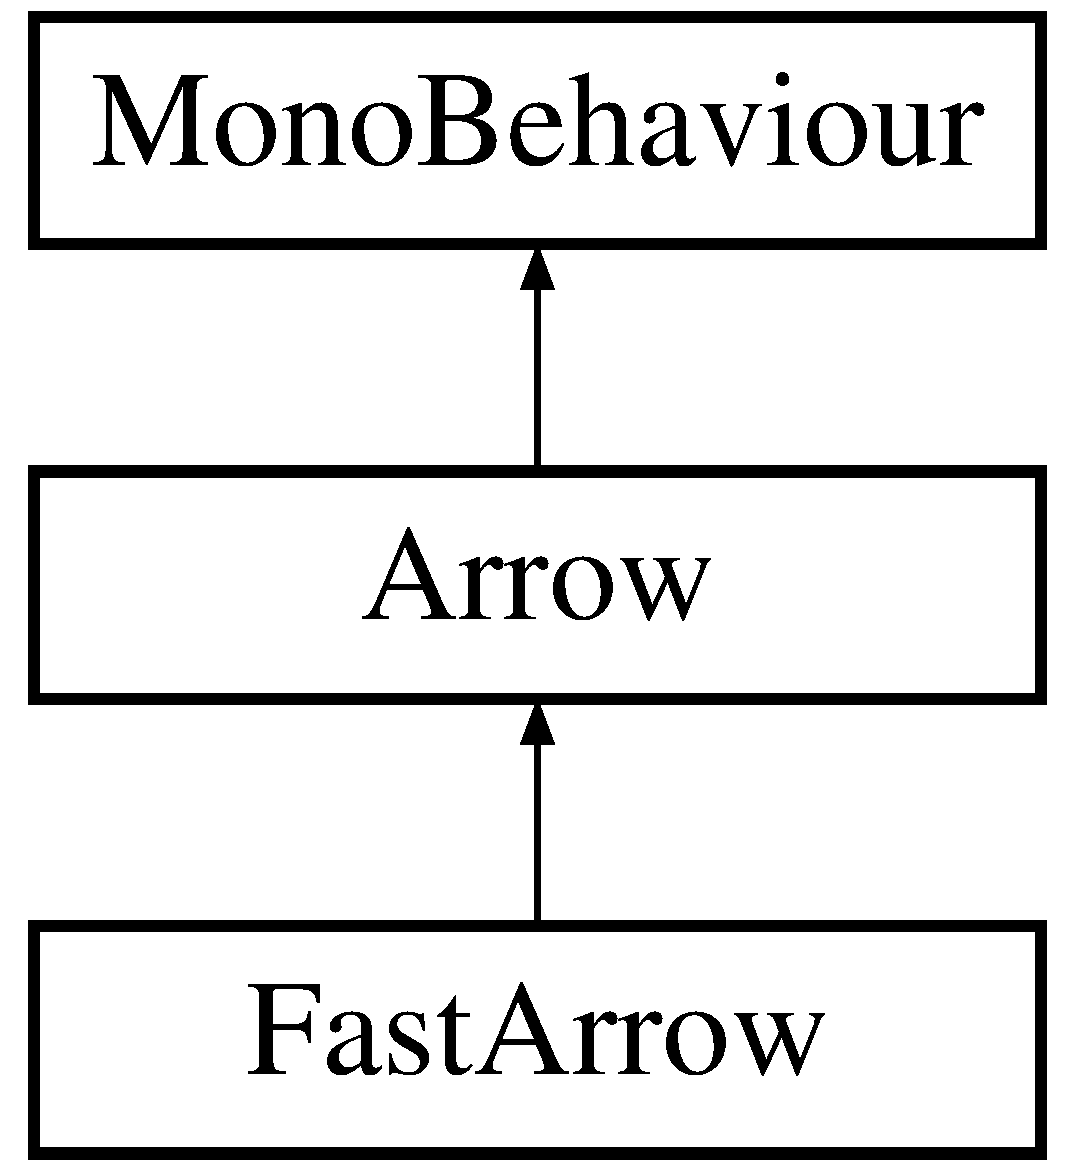
\includegraphics[height=3.000000cm]{class_fast_arrow}
\end{center}
\end{figure}
\subsection*{Private Member Functions}
\begin{DoxyCompactItemize}
\item 
new void \hyperlink{class_fast_arrow_a112df0c78fbcd99d22fc083c08e785de}{Start} ()
\item 
\mbox{\Hypertarget{class_fast_arrow_a4821a5e4ca53ebc904663395ee312061}\label{class_fast_arrow_a4821a5e4ca53ebc904663395ee312061}} 
void {\bfseries Update} ()
\end{DoxyCompactItemize}
\subsection*{Private Attributes}
\begin{DoxyCompactItemize}
\item 
\mbox{\Hypertarget{class_fast_arrow_aca9b777b6e4c2b4c611aec0433c2502d}\label{class_fast_arrow_aca9b777b6e4c2b4c611aec0433c2502d}} 
\hyperlink{class_arrow}{Arrow} {\bfseries Base\+Arrow}
\end{DoxyCompactItemize}
\subsection*{Additional Inherited Members}


\subsection{Detailed Description}
A faster moving arrow! Same as basic\+Arrow, except a different prefab with more speed as a default \begin{DoxyNote}{Note}
Prefab class 
\end{DoxyNote}


\subsection{Member Function Documentation}
\mbox{\Hypertarget{class_fast_arrow_a112df0c78fbcd99d22fc083c08e785de}\label{class_fast_arrow_a112df0c78fbcd99d22fc083c08e785de}} 
\index{Fast\+Arrow@{Fast\+Arrow}!Start@{Start}}
\index{Start@{Start}!Fast\+Arrow@{Fast\+Arrow}}
\subsubsection{\texorpdfstring{Start()}{Start()}}
{\footnotesize\ttfamily new void Fast\+Arrow.\+Start (\begin{DoxyParamCaption}{ }\end{DoxyParamCaption})\hspace{0.3cm}{\ttfamily [private]}}

\begin{DoxyPostcond}{Postcondition}
calls Base\+Arrow.\+Start(), then the parent class handels everything else. 
\end{DoxyPostcond}
\begin{DoxyNote}{Note}
it appears that this needs to be called otherwise the object won\textquotesingle{}t instantiate it\textquotesingle{}s parent class 
\end{DoxyNote}


The documentation for this class was generated from the following file\+:\begin{DoxyCompactItemize}
\item 
Assets/\+Scripts/\+Arrows/Fast\+Arrow.\+cs\end{DoxyCompactItemize}

\hypertarget{class_game_controller}{}\section{Game\+Controller Class Reference}
\label{class_game_controller}\index{Game\+Controller@{Game\+Controller}}
Inheritance diagram for Game\+Controller\+:\begin{figure}[H]
\begin{center}
\leavevmode
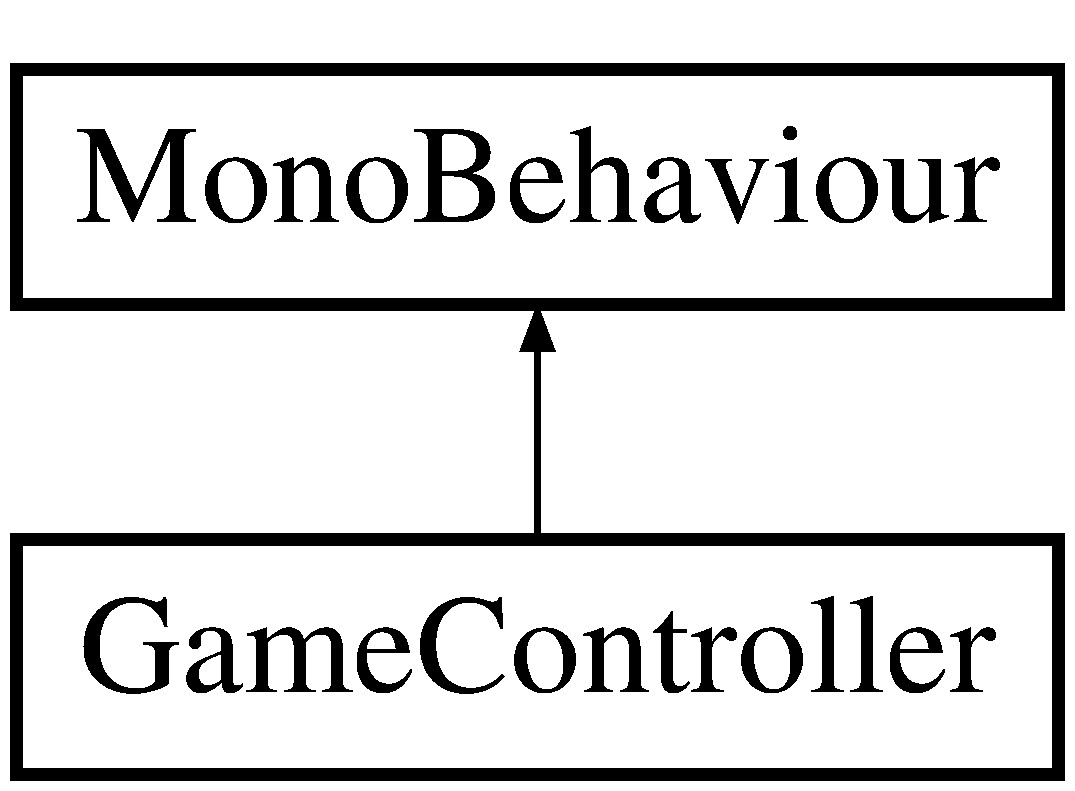
\includegraphics[height=2.000000cm]{class_game_controller}
\end{center}
\end{figure}
\subsection*{Public Member Functions}
\begin{DoxyCompactItemize}
\item 
void \hyperlink{class_game_controller_a0b2f5dd3890fd4897ca83421d9ce439c}{Toggle\+Pause\+Menu} ()
\end{DoxyCompactItemize}
\subsection*{Public Attributes}
\begin{DoxyCompactItemize}
\item 
\mbox{\Hypertarget{class_game_controller_ae49cd9c319e5d5ad8e4346f74fcd1ab4}\label{class_game_controller_ae49cd9c319e5d5ad8e4346f74fcd1ab4}} 
Game\+Object \hyperlink{class_game_controller_ae49cd9c319e5d5ad8e4346f74fcd1ab4}{Osu\+Circle}
\begin{DoxyCompactList}\small\item\em \hyperlink{class_osu_circle}{Osu\+Circle} gameobject to be instantiated. \end{DoxyCompactList}\item 
\mbox{\Hypertarget{class_game_controller_a3ce5989e4c40bdf139e70c9985559a78}\label{class_game_controller_a3ce5989e4c40bdf139e70c9985559a78}} 
bool \hyperlink{class_game_controller_a3ce5989e4c40bdf139e70c9985559a78}{player\+Is\+Firing}
\begin{DoxyCompactList}\small\item\em boolean to handle firing control \end{DoxyCompactList}\item 
\mbox{\Hypertarget{class_game_controller_a4f83ac6f51abe164a979acdf01318905}\label{class_game_controller_a4f83ac6f51abe164a979acdf01318905}} 
bool \hyperlink{class_game_controller_a4f83ac6f51abe164a979acdf01318905}{is\+Paused}
\begin{DoxyCompactList}\small\item\em boolean to handel pause controll \end{DoxyCompactList}\item 
\mbox{\Hypertarget{class_game_controller_aef62bc59c2244238483cb489b74352ac}\label{class_game_controller_aef62bc59c2244238483cb489b74352ac}} 
\hyperlink{class_pause_menu}{Pause\+Menu} \hyperlink{class_game_controller_aef62bc59c2244238483cb489b74352ac}{Menu}
\begin{DoxyCompactList}\small\item\em \hyperlink{class_pause_menu}{Pause\+Menu} object to handle pausing. \end{DoxyCompactList}\end{DoxyCompactItemize}
\subsection*{Private Member Functions}
\begin{DoxyCompactItemize}
\item 
void \hyperlink{class_game_controller_a97788a7aa0f09c8d748781683e5f045b}{Start} ()
\item 
void \hyperlink{class_game_controller_a5a89277529cadb49af7d55eba3bbf056}{Update} ()
\end{DoxyCompactItemize}
\subsection*{Private Attributes}
\begin{DoxyCompactItemize}
\item 
\mbox{\Hypertarget{class_game_controller_a3de58fb8ba542b1777de9f3bd9bb0977}\label{class_game_controller_a3de58fb8ba542b1777de9f3bd9bb0977}} 
\hyperlink{class_spell_controller}{Spell\+Controller} \hyperlink{class_game_controller_a3de58fb8ba542b1777de9f3bd9bb0977}{spell\+Controller}
\begin{DoxyCompactList}\small\item\em \hyperlink{class_spell_controller}{Spell\+Controller} in scene to communicate with. \end{DoxyCompactList}\item 
\mbox{\Hypertarget{class_game_controller_a2b44559411b7d7d6b52481b7f7b75852}\label{class_game_controller_a2b44559411b7d7d6b52481b7f7b75852}} 
\hyperlink{class_u_i_controller}{U\+I\+Controller} \hyperlink{class_game_controller_a2b44559411b7d7d6b52481b7f7b75852}{UI}
\begin{DoxyCompactList}\small\item\em \hyperlink{class_u_i_controller}{U\+I\+Controller} object to handle other UI related events. \end{DoxyCompactList}\end{DoxyCompactItemize}


\subsection{Detailed Description}
Manages overall gameflow and inputs not directly linked to player 

\subsection{Member Function Documentation}
\mbox{\Hypertarget{class_game_controller_a97788a7aa0f09c8d748781683e5f045b}\label{class_game_controller_a97788a7aa0f09c8d748781683e5f045b}} 
\index{Game\+Controller@{Game\+Controller}!Start@{Start}}
\index{Start@{Start}!Game\+Controller@{Game\+Controller}}
\subsubsection{\texorpdfstring{Start()}{Start()}}
{\footnotesize\ttfamily void Game\+Controller.\+Start (\begin{DoxyParamCaption}{ }\end{DoxyParamCaption})\hspace{0.3cm}{\ttfamily [private]}}

Sets default members and privates. \mbox{\Hypertarget{class_game_controller_a0b2f5dd3890fd4897ca83421d9ce439c}\label{class_game_controller_a0b2f5dd3890fd4897ca83421d9ce439c}} 
\index{Game\+Controller@{Game\+Controller}!Toggle\+Pause\+Menu@{Toggle\+Pause\+Menu}}
\index{Toggle\+Pause\+Menu@{Toggle\+Pause\+Menu}!Game\+Controller@{Game\+Controller}}
\subsubsection{\texorpdfstring{Toggle\+Pause\+Menu()}{TogglePauseMenu()}}
{\footnotesize\ttfamily void Game\+Controller.\+Toggle\+Pause\+Menu (\begin{DoxyParamCaption}{ }\end{DoxyParamCaption})}

Handles pausemenu interaction. stops time (however not updates) Becareful how we set object updates! \mbox{\Hypertarget{class_game_controller_a5a89277529cadb49af7d55eba3bbf056}\label{class_game_controller_a5a89277529cadb49af7d55eba3bbf056}} 
\index{Game\+Controller@{Game\+Controller}!Update@{Update}}
\index{Update@{Update}!Game\+Controller@{Game\+Controller}}
\subsubsection{\texorpdfstring{Update()}{Update()}}
{\footnotesize\ttfamily void Game\+Controller.\+Update (\begin{DoxyParamCaption}{ }\end{DoxyParamCaption})\hspace{0.3cm}{\ttfamily [private]}}

Checks for any updates that need to be applied to game world such as if a player has held down the shoot button Unused Osucircle testing function

\begin{DoxyNote}{Note}
Fire2 is the default mousebutton 2 on PC, but can be used on other platforms when defining global controlls 
\end{DoxyNote}


The documentation for this class was generated from the following file\+:\begin{DoxyCompactItemize}
\item 
Assets/\+Scripts/\+Controllers/Game\+Controller.\+cs\end{DoxyCompactItemize}

\hypertarget{class_item_spawner}{}\section{Item\+Spawner Class Reference}
\label{class_item_spawner}\index{Item\+Spawner@{Item\+Spawner}}
Inheritance diagram for Item\+Spawner\+:\begin{figure}[H]
\begin{center}
\leavevmode
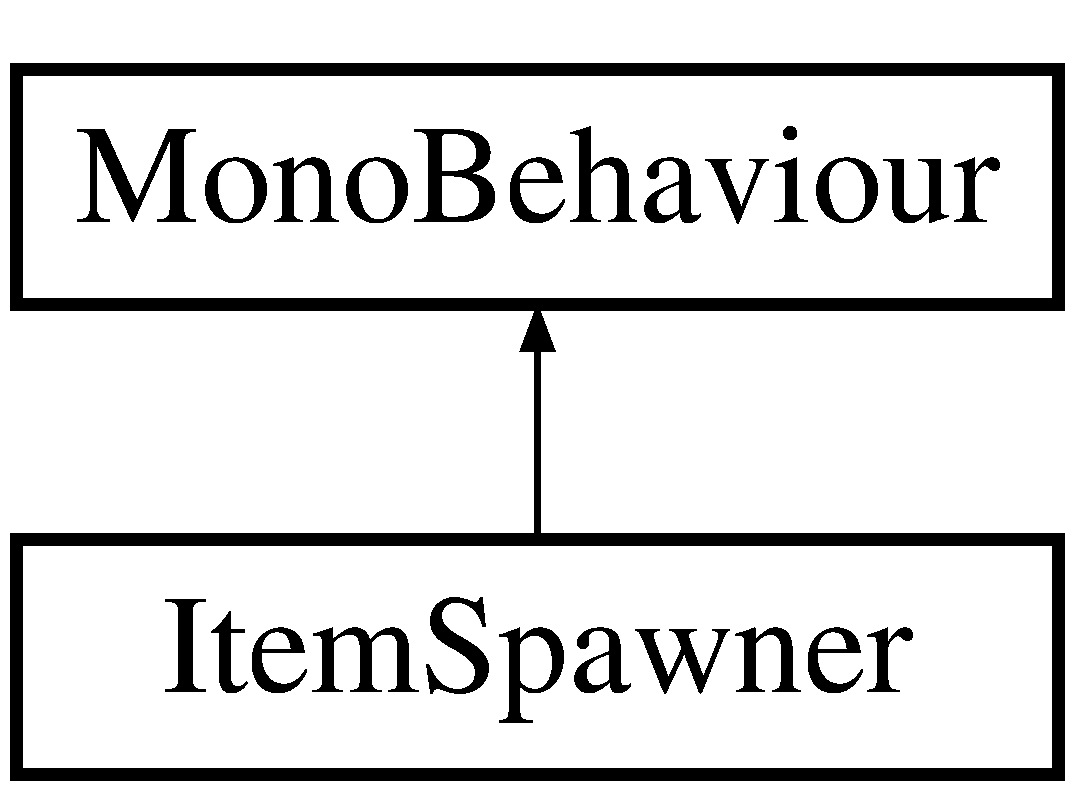
\includegraphics[height=2.000000cm]{class_item_spawner}
\end{center}
\end{figure}
\subsection*{Public Attributes}
\begin{DoxyCompactItemize}
\item 
\mbox{\Hypertarget{class_item_spawner_a7798ea5cc02f82bbd0828483af3ab744}\label{class_item_spawner_a7798ea5cc02f82bbd0828483af3ab744}} 
List$<$ Game\+Object $>$ \hyperlink{class_item_spawner_a7798ea5cc02f82bbd0828483af3ab744}{items}
\begin{DoxyCompactList}\small\item\em list of all items to spawn in this spawner \end{DoxyCompactList}\end{DoxyCompactItemize}
\subsection*{Private Member Functions}
\begin{DoxyCompactItemize}
\item 
void \hyperlink{class_item_spawner_a8747f1740ce252a8676120567abd16e6}{Start} ()
\item 
void \hyperlink{class_item_spawner_a2103c51aae4e7fbf8187e91767b2660c}{Spawn\+Item} ()
\end{DoxyCompactItemize}


\subsection{Detailed Description}
Spawns items perodically. Based of score 

\subsection{Member Function Documentation}
\mbox{\Hypertarget{class_item_spawner_a2103c51aae4e7fbf8187e91767b2660c}\label{class_item_spawner_a2103c51aae4e7fbf8187e91767b2660c}} 
\index{Item\+Spawner@{Item\+Spawner}!Spawn\+Item@{Spawn\+Item}}
\index{Spawn\+Item@{Spawn\+Item}!Item\+Spawner@{Item\+Spawner}}
\subsubsection{\texorpdfstring{Spawn\+Item()}{SpawnItem()}}
{\footnotesize\ttfamily void Item\+Spawner.\+Spawn\+Item (\begin{DoxyParamCaption}{ }\end{DoxyParamCaption})\hspace{0.3cm}{\ttfamily [private]}}

Spawns a random item in on the spawner $<$ \begin{DoxyNote}{Note}
adds a random direction to the object so it\textquotesingle{}s not stuck in the middle of the well. 
\end{DoxyNote}
\mbox{\Hypertarget{class_item_spawner_a8747f1740ce252a8676120567abd16e6}\label{class_item_spawner_a8747f1740ce252a8676120567abd16e6}} 
\index{Item\+Spawner@{Item\+Spawner}!Start@{Start}}
\index{Start@{Start}!Item\+Spawner@{Item\+Spawner}}
\subsubsection{\texorpdfstring{Start()}{Start()}}
{\footnotesize\ttfamily void Item\+Spawner.\+Start (\begin{DoxyParamCaption}{ }\end{DoxyParamCaption})\hspace{0.3cm}{\ttfamily [private]}}

Starts Spawning sequence in repitition and also sets lays to ignore 

The documentation for this class was generated from the following file\+:\begin{DoxyCompactItemize}
\item 
Assets/\+Scripts/\+Entities/Item\+Spawner.\+cs\end{DoxyCompactItemize}

\hypertarget{class_load_scene_on_click}{}\section{Load\+Scene\+On\+Click Class Reference}
\label{class_load_scene_on_click}\index{Load\+Scene\+On\+Click@{Load\+Scene\+On\+Click}}
Inheritance diagram for Load\+Scene\+On\+Click\+:\begin{figure}[H]
\begin{center}
\leavevmode
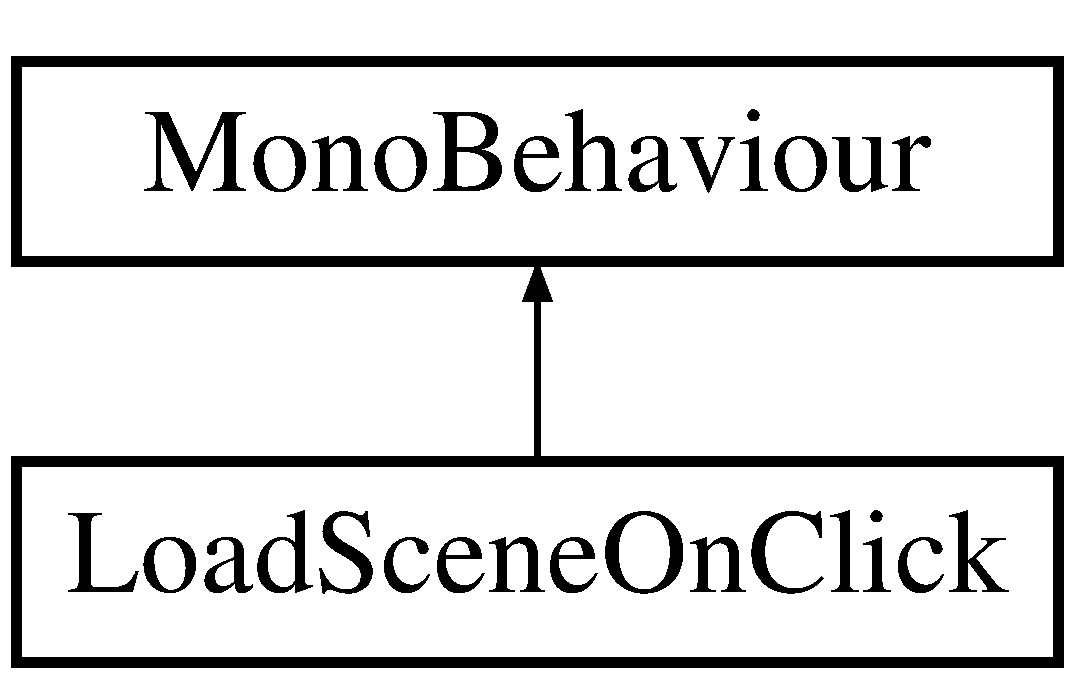
\includegraphics[height=2.000000cm]{class_load_scene_on_click}
\end{center}
\end{figure}
\subsection*{Public Member Functions}
\begin{DoxyCompactItemize}
\item 
void \hyperlink{class_load_scene_on_click_a2e42d46710af3967cbfcdf5b87fb61f2}{Load\+By\+Index} (int Scene\+Index)
\end{DoxyCompactItemize}


\subsection{Detailed Description}
Handles differenct scenes 

\subsection{Member Function Documentation}
\mbox{\Hypertarget{class_load_scene_on_click_a2e42d46710af3967cbfcdf5b87fb61f2}\label{class_load_scene_on_click_a2e42d46710af3967cbfcdf5b87fb61f2}} 
\index{Load\+Scene\+On\+Click@{Load\+Scene\+On\+Click}!Load\+By\+Index@{Load\+By\+Index}}
\index{Load\+By\+Index@{Load\+By\+Index}!Load\+Scene\+On\+Click@{Load\+Scene\+On\+Click}}
\subsubsection{\texorpdfstring{Load\+By\+Index()}{LoadByIndex()}}
{\footnotesize\ttfamily void Load\+Scene\+On\+Click.\+Load\+By\+Index (\begin{DoxyParamCaption}\item[{int}]{Scene\+Index }\end{DoxyParamCaption})}

Loads a scene by index 
\begin{DoxyParams}{Parameters}
{\em Scene\+Index} & is the value of the scene assigned by build order \\
\hline
\end{DoxyParams}


The documentation for this class was generated from the following file\+:\begin{DoxyCompactItemize}
\item 
Assets/\+Scripts/\+U\+I/\+Menu/Load\+Scene\+On\+Click.\+cs\end{DoxyCompactItemize}

\hypertarget{class_mob1_movement}{}\section{Mob1\+Movement Class Reference}
\label{class_mob1_movement}\index{Mob1\+Movement@{Mob1\+Movement}}
Inheritance diagram for Mob1\+Movement\+:\begin{figure}[H]
\begin{center}
\leavevmode
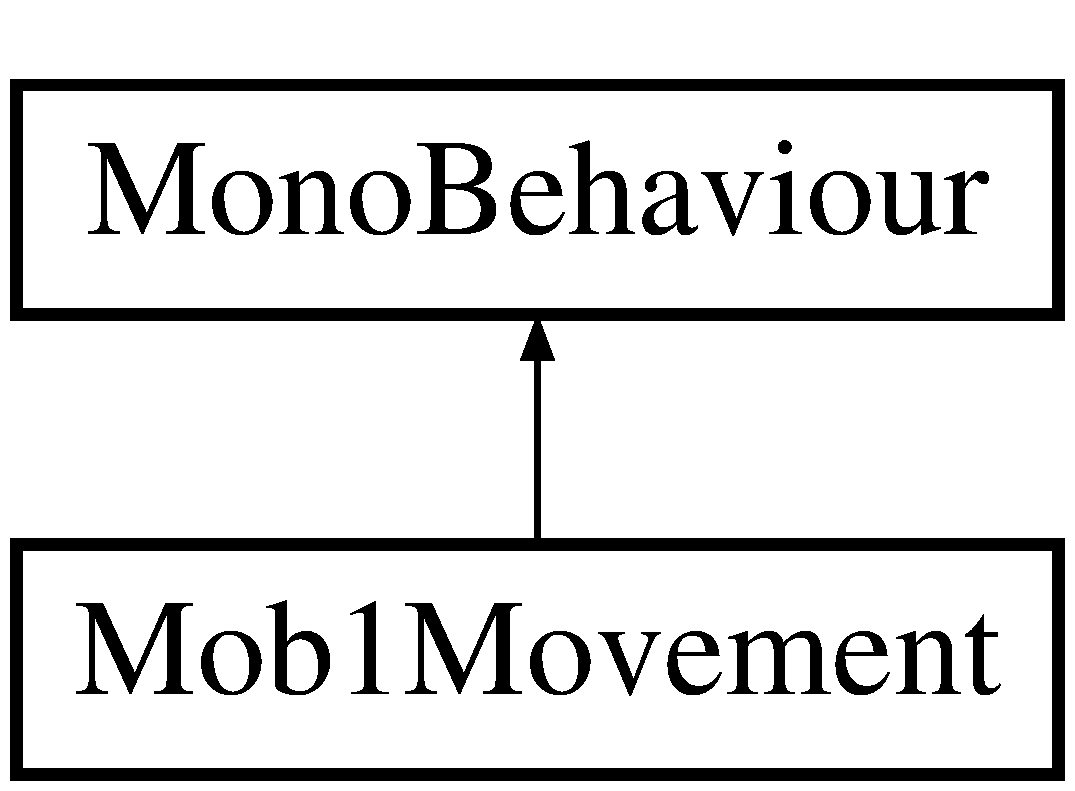
\includegraphics[height=2.000000cm]{class_mob1_movement}
\end{center}
\end{figure}
\subsection*{Public Attributes}
\begin{DoxyCompactItemize}
\item 
\mbox{\Hypertarget{class_mob1_movement_a60cea12c3ca0514b7fa3bdd78fccc257}\label{class_mob1_movement_a60cea12c3ca0514b7fa3bdd78fccc257}} 
Game\+Object {\bfseries Mob\+Canvas}
\item 
\mbox{\Hypertarget{class_mob1_movement_a90c9578db347384411e4ad1f8ecd0133}\label{class_mob1_movement_a90c9578db347384411e4ad1f8ecd0133}} 
Game\+Object {\bfseries Mob\+Text\+Prefab}
\item 
\mbox{\Hypertarget{class_mob1_movement_aa5d29d107c8b3c137f630e80c06a6f30}\label{class_mob1_movement_aa5d29d107c8b3c137f630e80c06a6f30}} 
float \hyperlink{class_mob1_movement_aa5d29d107c8b3c137f630e80c06a6f30}{speed}
\begin{DoxyCompactList}\small\item\em speed which the mob approaches the player \end{DoxyCompactList}\end{DoxyCompactItemize}
\subsection*{Private Member Functions}
\begin{DoxyCompactItemize}
\item 
void \hyperlink{class_mob1_movement_ab5d6209e3082865eb69e197997e7c8f7}{Awake} ()
\item 
void \hyperlink{class_mob1_movement_a788bc296f79b07051e91a3c1d1613bc9}{Update} ()
\item 
void \hyperlink{class_mob1_movement_a208b9f2f72d057c44055af58371bdfd1}{Damage\+Hit} ()
\item 
void \hyperlink{class_mob1_movement_a8c36ef4e56bc37704d47635c444a07c6}{Damage\+Text\+Init} (string damage)
\item 
void \hyperlink{class_mob1_movement_a77cf67d8073a810fd269199883b485b6}{Stabilize\+Canvas} ()
\begin{DoxyCompactList}\small\item\em $<$ Stabilizes the canvas with respect to the camera because the player is moving \end{DoxyCompactList}\end{DoxyCompactItemize}
\subsection*{Private Attributes}
\begin{DoxyCompactItemize}
\item 
\mbox{\Hypertarget{class_mob1_movement_a7d4076faee2feead1c09d2a670aa24c5}\label{class_mob1_movement_a7d4076faee2feead1c09d2a670aa24c5}} 
Transform \hyperlink{class_mob1_movement_a7d4076faee2feead1c09d2a670aa24c5}{player}
\begin{DoxyCompactList}\small\item\em \hyperlink{class_player}{Player}\textquotesingle{}s current position. \end{DoxyCompactList}\item 
\mbox{\Hypertarget{class_mob1_movement_a48a34641232183ed3da4641f82dd4f20}\label{class_mob1_movement_a48a34641232183ed3da4641f82dd4f20}} 
Unity\+Engine.\+A\+I.\+Nav\+Mesh\+Agent {\bfseries nav}
\end{DoxyCompactItemize}


\subsection{Detailed Description}
Basic mob class This mob follows the player directly 

\subsection{Member Function Documentation}
\mbox{\Hypertarget{class_mob1_movement_ab5d6209e3082865eb69e197997e7c8f7}\label{class_mob1_movement_ab5d6209e3082865eb69e197997e7c8f7}} 
\index{Mob1\+Movement@{Mob1\+Movement}!Awake@{Awake}}
\index{Awake@{Awake}!Mob1\+Movement@{Mob1\+Movement}}
\subsubsection{\texorpdfstring{Awake()}{Awake()}}
{\footnotesize\ttfamily void Mob1\+Movement.\+Awake (\begin{DoxyParamCaption}{ }\end{DoxyParamCaption})\hspace{0.3cm}{\ttfamily [private]}}

Sets member values \mbox{\Hypertarget{class_mob1_movement_a208b9f2f72d057c44055af58371bdfd1}\label{class_mob1_movement_a208b9f2f72d057c44055af58371bdfd1}} 
\index{Mob1\+Movement@{Mob1\+Movement}!Damage\+Hit@{Damage\+Hit}}
\index{Damage\+Hit@{Damage\+Hit}!Mob1\+Movement@{Mob1\+Movement}}
\subsubsection{\texorpdfstring{Damage\+Hit()}{DamageHit()}}
{\footnotesize\ttfamily void Mob1\+Movement.\+Damage\+Hit (\begin{DoxyParamCaption}{ }\end{DoxyParamCaption})\hspace{0.3cm}{\ttfamily [private]}}

Do health calculations with damage on health Give Health to Damage\+Text\+Init using To\+String method \mbox{\Hypertarget{class_mob1_movement_a8c36ef4e56bc37704d47635c444a07c6}\label{class_mob1_movement_a8c36ef4e56bc37704d47635c444a07c6}} 
\index{Mob1\+Movement@{Mob1\+Movement}!Damage\+Text\+Init@{Damage\+Text\+Init}}
\index{Damage\+Text\+Init@{Damage\+Text\+Init}!Mob1\+Movement@{Mob1\+Movement}}
\subsubsection{\texorpdfstring{Damage\+Text\+Init()}{DamageTextInit()}}
{\footnotesize\ttfamily void Mob1\+Movement.\+Damage\+Text\+Init (\begin{DoxyParamCaption}\item[{string}]{damage }\end{DoxyParamCaption})\hspace{0.3cm}{\ttfamily [private]}}

Creates Damage text on hit \mbox{\Hypertarget{class_mob1_movement_a77cf67d8073a810fd269199883b485b6}\label{class_mob1_movement_a77cf67d8073a810fd269199883b485b6}} 
\index{Mob1\+Movement@{Mob1\+Movement}!Stabilize\+Canvas@{Stabilize\+Canvas}}
\index{Stabilize\+Canvas@{Stabilize\+Canvas}!Mob1\+Movement@{Mob1\+Movement}}
\subsubsection{\texorpdfstring{Stabilize\+Canvas()}{StabilizeCanvas()}}
{\footnotesize\ttfamily void Mob1\+Movement.\+Stabilize\+Canvas (\begin{DoxyParamCaption}{ }\end{DoxyParamCaption})\hspace{0.3cm}{\ttfamily [private]}}



$<$ Stabilizes the canvas with respect to the camera because the player is moving 

Smooths the damage text\textquotesingle{}s canvas to decrease jitter \begin{DoxyNote}{Note}
52.\+0f for the camera angle and stable\+\_\+y to make up for rotation of the player 
\end{DoxyNote}
\mbox{\Hypertarget{class_mob1_movement_a788bc296f79b07051e91a3c1d1613bc9}\label{class_mob1_movement_a788bc296f79b07051e91a3c1d1613bc9}} 
\index{Mob1\+Movement@{Mob1\+Movement}!Update@{Update}}
\index{Update@{Update}!Mob1\+Movement@{Mob1\+Movement}}
\subsubsection{\texorpdfstring{Update()}{Update()}}
{\footnotesize\ttfamily void Mob1\+Movement.\+Update (\begin{DoxyParamCaption}{ }\end{DoxyParamCaption})\hspace{0.3cm}{\ttfamily [private]}}

Updates all members and checks for test \char`\"{}\+T\char`\"{} input for damage 

The documentation for this class was generated from the following file\+:\begin{DoxyCompactItemize}
\item 
Assets/\+Scripts/\+Entities/Mob1\+Movement.\+cs\end{DoxyCompactItemize}

\hypertarget{class_mob2_movement}{}\section{Mob2\+Movement Class Reference}
\label{class_mob2_movement}\index{Mob2\+Movement@{Mob2\+Movement}}
Inheritance diagram for Mob2\+Movement\+:\begin{figure}[H]
\begin{center}
\leavevmode
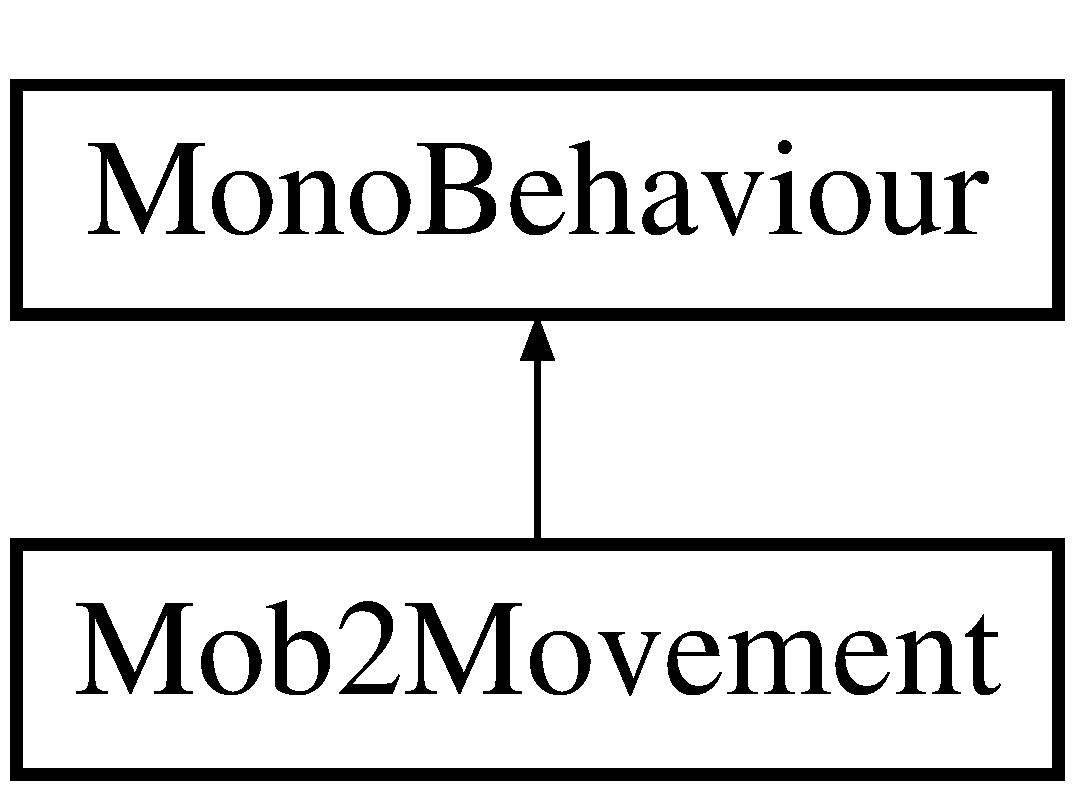
\includegraphics[height=2.000000cm]{class_mob2_movement}
\end{center}
\end{figure}
\subsection*{Public Attributes}
\begin{DoxyCompactItemize}
\item 
\mbox{\Hypertarget{class_mob2_movement_a562eaed5122c4ab12bd8e6da9ee5cae4}\label{class_mob2_movement_a562eaed5122c4ab12bd8e6da9ee5cae4}} 
float \hyperlink{class_mob2_movement_a562eaed5122c4ab12bd8e6da9ee5cae4}{jump\+Rate} = 2f
\begin{DoxyCompactList}\small\item\em Frequency of jumping. \end{DoxyCompactList}\item 
\mbox{\Hypertarget{class_mob2_movement_a55cced54062a86039e52800d49c65f18}\label{class_mob2_movement_a55cced54062a86039e52800d49c65f18}} 
float \hyperlink{class_mob2_movement_a55cced54062a86039e52800d49c65f18}{jump\+Height} = 1000f
\begin{DoxyCompactList}\small\item\em force of jumping \end{DoxyCompactList}\end{DoxyCompactItemize}
\subsection*{Private Member Functions}
\begin{DoxyCompactItemize}
\item 
void \hyperlink{class_mob2_movement_a1caeb0925d5a847a3458ba312c35adb9}{Awake} ()
\item 
void \hyperlink{class_mob2_movement_ad5700e3c04953999dc85ba86cbcf889d}{Update} ()
\item 
void \hyperlink{class_mob2_movement_aedc7ef856890634eafcb09ed1e6d0a5f}{Jump} ()
\end{DoxyCompactItemize}
\subsection*{Private Attributes}
\begin{DoxyCompactItemize}
\item 
\mbox{\Hypertarget{class_mob2_movement_adba86d6852cafaebc8c24d03c5060a79}\label{class_mob2_movement_adba86d6852cafaebc8c24d03c5060a79}} 
Transform \hyperlink{class_mob2_movement_adba86d6852cafaebc8c24d03c5060a79}{player}
\begin{DoxyCompactList}\small\item\em \hyperlink{class_player}{Player} position/transform. \end{DoxyCompactList}\item 
\mbox{\Hypertarget{class_mob2_movement_a9d18fd4ab57a4b254e41572a5e51221a}\label{class_mob2_movement_a9d18fd4ab57a4b254e41572a5e51221a}} 
Nav\+Mesh\+Agent {\bfseries nav}
\item 
\mbox{\Hypertarget{class_mob2_movement_a277e1f62e34bfe7d2992de75b515c15d}\label{class_mob2_movement_a277e1f62e34bfe7d2992de75b515c15d}} 
Rigidbody {\bfseries rb}
\item 
\mbox{\Hypertarget{class_mob2_movement_ab46f0903ccfe3b8a8a8d958cb9891bc8}\label{class_mob2_movement_ab46f0903ccfe3b8a8a8d958cb9891bc8}} 
Animator {\bfseries anim}
\end{DoxyCompactItemize}


\subsection{Detailed Description}
This mob Occasionally jumps at the player 

\subsection{Member Function Documentation}
\mbox{\Hypertarget{class_mob2_movement_a1caeb0925d5a847a3458ba312c35adb9}\label{class_mob2_movement_a1caeb0925d5a847a3458ba312c35adb9}} 
\index{Mob2\+Movement@{Mob2\+Movement}!Awake@{Awake}}
\index{Awake@{Awake}!Mob2\+Movement@{Mob2\+Movement}}
\subsubsection{\texorpdfstring{Awake()}{Awake()}}
{\footnotesize\ttfamily void Mob2\+Movement.\+Awake (\begin{DoxyParamCaption}{ }\end{DoxyParamCaption})\hspace{0.3cm}{\ttfamily [private]}}

Sets member values \mbox{\Hypertarget{class_mob2_movement_aedc7ef856890634eafcb09ed1e6d0a5f}\label{class_mob2_movement_aedc7ef856890634eafcb09ed1e6d0a5f}} 
\index{Mob2\+Movement@{Mob2\+Movement}!Jump@{Jump}}
\index{Jump@{Jump}!Mob2\+Movement@{Mob2\+Movement}}
\subsubsection{\texorpdfstring{Jump()}{Jump()}}
{\footnotesize\ttfamily void Mob2\+Movement.\+Jump (\begin{DoxyParamCaption}{ }\end{DoxyParamCaption})\hspace{0.3cm}{\ttfamily [private]}}

Unity Physics engine calculation to jump at the player\textquotesingle{}s current location Animation for Surround attack \begin{DoxyNote}{Note}
since it looks neat 
\end{DoxyNote}
\mbox{\Hypertarget{class_mob2_movement_ad5700e3c04953999dc85ba86cbcf889d}\label{class_mob2_movement_ad5700e3c04953999dc85ba86cbcf889d}} 
\index{Mob2\+Movement@{Mob2\+Movement}!Update@{Update}}
\index{Update@{Update}!Mob2\+Movement@{Mob2\+Movement}}
\subsubsection{\texorpdfstring{Update()}{Update()}}
{\footnotesize\ttfamily void Mob2\+Movement.\+Update (\begin{DoxyParamCaption}{ }\end{DoxyParamCaption})\hspace{0.3cm}{\ttfamily [private]}}

Constantly rotate to look at player \begin{DoxyNote}{Note}
since this mob only moves with jumps, this is used. 
\end{DoxyNote}


The documentation for this class was generated from the following file\+:\begin{DoxyCompactItemize}
\item 
Assets/\+Scripts/\+Entities/Mob2\+Movement.\+cs\end{DoxyCompactItemize}

\hypertarget{class_mob_health}{}\section{Mob\+Health Class Reference}
\label{class_mob_health}\index{Mob\+Health@{Mob\+Health}}
Inheritance diagram for Mob\+Health\+:\begin{figure}[H]
\begin{center}
\leavevmode
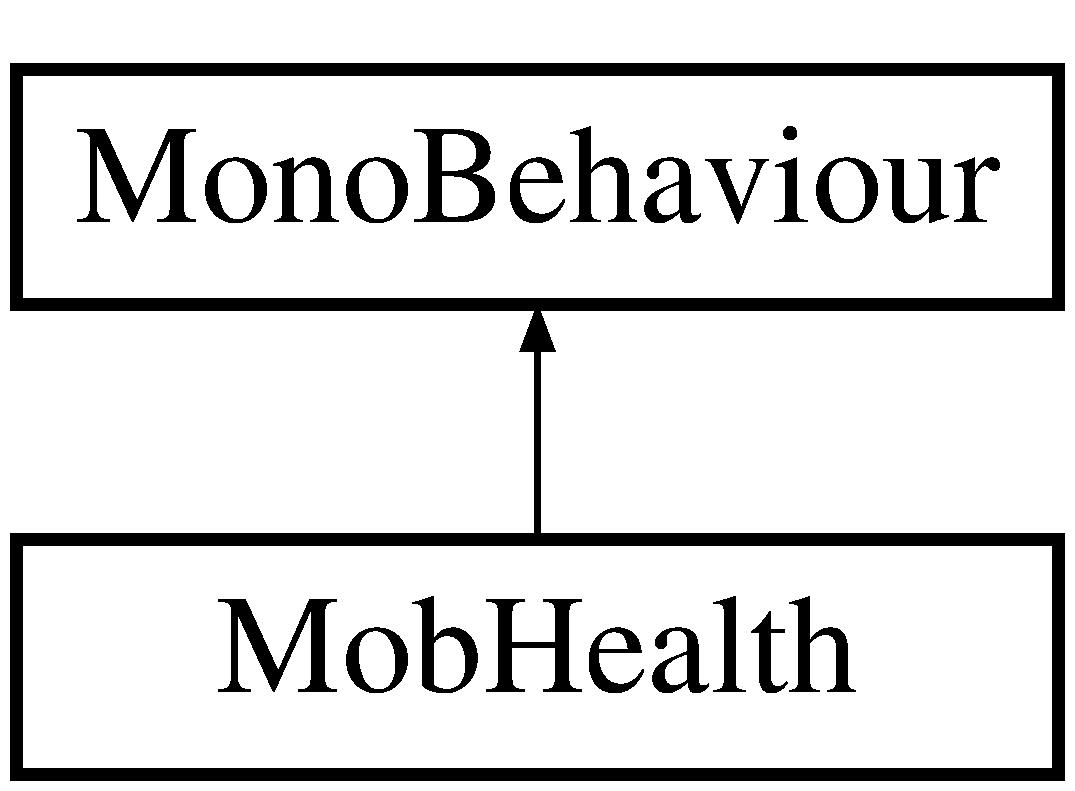
\includegraphics[height=2.000000cm]{class_mob_health}
\end{center}
\end{figure}
\subsection*{Public Member Functions}
\begin{DoxyCompactItemize}
\item 
void \hyperlink{class_mob_health_adaf878419692a8b6a16f8f3861a6c74e}{Do\+Damage} (float dmg)
\item 
void \hyperlink{class_mob_health_abcc0a1a5fef542a2c5f83e3d80d21d18}{Start\+Burn} (float dmg, int burns)
\item 
I\+Enumerator \hyperlink{class_mob_health_a90c10dc6ba571545b3d466ec83ebf6e7}{Apply\+Burn} (float dmg, int burns\+Left)
\item 
void \hyperlink{class_mob_health_ac4b90844fdf1be4b5fad4693c48bd61f}{Apply\+Freeze} (float dmg, float time)
\item 
void \hyperlink{class_mob_health_a7374507ad90db5ced9395476a3943230}{Apply\+Slow} (float dmg, float slow\+Mult)
\end{DoxyCompactItemize}
\subsection*{Public Attributes}
\begin{DoxyCompactItemize}
\item 
\mbox{\Hypertarget{class_mob_health_acf92ca7925059c25691b1a6fdc921e3f}\label{class_mob_health_acf92ca7925059c25691b1a6fdc921e3f}} 
float \hyperlink{class_mob_health_acf92ca7925059c25691b1a6fdc921e3f}{health} = 10f
\begin{DoxyCompactList}\small\item\em Base health. \end{DoxyCompactList}\item 
\mbox{\Hypertarget{class_mob_health_a766429dd6a72c403a371b87e3522fa43}\label{class_mob_health_a766429dd6a72c403a371b87e3522fa43}} 
float \hyperlink{class_mob_health_a766429dd6a72c403a371b87e3522fa43}{cur\+Health}
\begin{DoxyCompactList}\small\item\em Health at any given moment. \end{DoxyCompactList}\item 
\mbox{\Hypertarget{class_mob_health_a08f875a009f447e245015e1df63b4bb4}\label{class_mob_health_a08f875a009f447e245015e1df63b4bb4}} 
Texture2D \hyperlink{class_mob_health_a08f875a009f447e245015e1df63b4bb4}{Hp\+Bar\+Texture}
\begin{DoxyCompactList}\small\item\em H\+P\+Bar texture. \end{DoxyCompactList}\item 
\mbox{\Hypertarget{class_mob_health_aa9c36ad6a31c1e07393b6e70f8b98caa}\label{class_mob_health_aa9c36ad6a31c1e07393b6e70f8b98caa}} 
Texture2D {\bfseries Hp\+Back\+Texture}
\item 
\mbox{\Hypertarget{class_mob_health_ad20b76297e42388a314f26e863acdf09}\label{class_mob_health_ad20b76297e42388a314f26e863acdf09}} 
Game\+Object \hyperlink{class_mob_health_ad20b76297e42388a314f26e863acdf09}{damage\+Text}
\begin{DoxyCompactList}\small\item\em Damage to show. \end{DoxyCompactList}\end{DoxyCompactItemize}
\subsection*{Private Member Functions}
\begin{DoxyCompactItemize}
\item 
void \hyperlink{class_mob_health_af397aaaf764c7338aa1a83714537a68a}{Start} ()
\item 
void \hyperlink{class_mob_health_a0652c8b5a2fcb5cb791eb26305425024}{Update} ()
\item 
void \hyperlink{class_mob_health_a13e17984b18c95b8e6d56f52f9e11a71}{Init\+Damage\+Text} (string str)
\item 
void \hyperlink{class_mob_health_aa6acd5f6aad4b4d621db7d927169cd70}{Unfreeze} ()
\item 
void \hyperlink{class_mob_health_aba4ed1f920f770c312d214e541620f9f}{Burn\+Effect} (float dmg)
\begin{DoxyCompactList}\small\item\em Test for Health Bar. \end{DoxyCompactList}\item 
\mbox{\Hypertarget{class_mob_health_ae30ec0b3661db3d9306ead156bcc90c2}\label{class_mob_health_ae30ec0b3661db3d9306ead156bcc90c2}} 
void {\bfseries On\+G\+UI} ()
\end{DoxyCompactItemize}
\subsection*{Private Attributes}
\begin{DoxyCompactItemize}
\item 
\mbox{\Hypertarget{class_mob_health_a62d5d74d1e5f66d626fc1e76f2be84cc}\label{class_mob_health_a62d5d74d1e5f66d626fc1e76f2be84cc}} 
\hyperlink{class_mob2_movement}{Mob2\+Movement} \hyperlink{class_mob_health_a62d5d74d1e5f66d626fc1e76f2be84cc}{movement2}
\begin{DoxyCompactList}\small\item\em Movement sceme for mob2. \end{DoxyCompactList}\item 
\mbox{\Hypertarget{class_mob_health_afb9d2d290a111506515407311408ed98}\label{class_mob_health_afb9d2d290a111506515407311408ed98}} 
Nav\+Mesh\+Agent \hyperlink{class_mob_health_afb9d2d290a111506515407311408ed98}{nav}
\begin{DoxyCompactList}\small\item\em Nav mesh of the land to use Unity\textquotesingle{}s Default pathing AI. \end{DoxyCompactList}\item 
\mbox{\Hypertarget{class_mob_health_ac5aa23c1785ac8bdde4ca35b04b8967a}\label{class_mob_health_ac5aa23c1785ac8bdde4ca35b04b8967a}} 
float \hyperlink{class_mob_health_ac5aa23c1785ac8bdde4ca35b04b8967a}{nav\+Speed}
\begin{DoxyCompactList}\small\item\em Speed. \end{DoxyCompactList}\item 
\mbox{\Hypertarget{class_mob_health_ac89dd915f414c757c3e0120ed403bb9b}\label{class_mob_health_ac89dd915f414c757c3e0120ed403bb9b}} 
bool \hyperlink{class_mob_health_ac89dd915f414c757c3e0120ed403bb9b}{already\+Slowed} = false
\begin{DoxyCompactList}\small\item\em Bool for speed. \end{DoxyCompactList}\item 
\mbox{\Hypertarget{class_mob_health_a452c19b63a316238a03bddd724a7e9ee}\label{class_mob_health_a452c19b63a316238a03bddd724a7e9ee}} 
float \hyperlink{class_mob_health_a452c19b63a316238a03bddd724a7e9ee}{hp\+Bar\+Length}
\begin{DoxyCompactList}\small\item\em Interacts with UI canvas to change depending on remaining HP. \end{DoxyCompactList}\item 
\mbox{\Hypertarget{class_mob_health_ade867811ed397c0701ffa21a446e92ac}\label{class_mob_health_ade867811ed397c0701ffa21a446e92ac}} 
Vector3 \hyperlink{class_mob_health_ade867811ed397c0701ffa21a446e92ac}{target}
\begin{DoxyCompactList}\small\item\em Target the mobthat\textquotesingle{}s attached is moving towards. \end{DoxyCompactList}\item 
\mbox{\Hypertarget{class_mob_health_a4e2637916ef423d557a89d0d7d50cb8f}\label{class_mob_health_a4e2637916ef423d557a89d0d7d50cb8f}} 
\hyperlink{class_u_i_controller}{U\+I\+Controller} \hyperlink{class_mob_health_a4e2637916ef423d557a89d0d7d50cb8f}{uic}
\begin{DoxyCompactList}\small\item\em \hyperlink{class_u_i_controller}{U\+I\+Controller}. \end{DoxyCompactList}\end{DoxyCompactItemize}


\subsection{Detailed Description}
Specific class for controlling Mob Health and status effects \begin{DoxyNote}{Note}
this Should not be a gameobject, but instead just a component attached to some gameobjects 
\end{DoxyNote}


\subsection{Member Function Documentation}
\mbox{\Hypertarget{class_mob_health_a90c10dc6ba571545b3d466ec83ebf6e7}\label{class_mob_health_a90c10dc6ba571545b3d466ec83ebf6e7}} 
\index{Mob\+Health@{Mob\+Health}!Apply\+Burn@{Apply\+Burn}}
\index{Apply\+Burn@{Apply\+Burn}!Mob\+Health@{Mob\+Health}}
\subsubsection{\texorpdfstring{Apply\+Burn()}{ApplyBurn()}}
{\footnotesize\ttfamily I\+Enumerator Mob\+Health.\+Apply\+Burn (\begin{DoxyParamCaption}\item[{float}]{dmg,  }\item[{int}]{burns\+Left }\end{DoxyParamCaption})}

I\+Enumerator to apply damage continiously... the \char`\"{}burning\char`\"{} effect 
\begin{DoxyParams}{Parameters}
{\em dmg} & initial damage \\
\hline
{\em burns\+Left} & how many loops to go through before expiring \\
\hline
\end{DoxyParams}
\mbox{\Hypertarget{class_mob_health_ac4b90844fdf1be4b5fad4693c48bd61f}\label{class_mob_health_ac4b90844fdf1be4b5fad4693c48bd61f}} 
\index{Mob\+Health@{Mob\+Health}!Apply\+Freeze@{Apply\+Freeze}}
\index{Apply\+Freeze@{Apply\+Freeze}!Mob\+Health@{Mob\+Health}}
\subsubsection{\texorpdfstring{Apply\+Freeze()}{ApplyFreeze()}}
{\footnotesize\ttfamily void Mob\+Health.\+Apply\+Freeze (\begin{DoxyParamCaption}\item[{float}]{dmg,  }\item[{float}]{time }\end{DoxyParamCaption})}

Applies Freeze effect to mob. 
\begin{DoxyParams}{Parameters}
{\em dmg} & initial Damage \\
\hline
{\em time} & duration of freeze \\
\hline
\end{DoxyParams}
\mbox{\Hypertarget{class_mob_health_a7374507ad90db5ced9395476a3943230}\label{class_mob_health_a7374507ad90db5ced9395476a3943230}} 
\index{Mob\+Health@{Mob\+Health}!Apply\+Slow@{Apply\+Slow}}
\index{Apply\+Slow@{Apply\+Slow}!Mob\+Health@{Mob\+Health}}
\subsubsection{\texorpdfstring{Apply\+Slow()}{ApplySlow()}}
{\footnotesize\ttfamily void Mob\+Health.\+Apply\+Slow (\begin{DoxyParamCaption}\item[{float}]{dmg,  }\item[{float}]{slow\+Mult }\end{DoxyParamCaption})}

Applies a slowing effect to the mob 
\begin{DoxyParams}{Parameters}
{\em dmg} & initial damage \\
\hline
{\em slow\+Mult} & the change to the speed multiplier of the mob \\
\hline
\end{DoxyParams}
\mbox{\Hypertarget{class_mob_health_aba4ed1f920f770c312d214e541620f9f}\label{class_mob_health_aba4ed1f920f770c312d214e541620f9f}} 
\index{Mob\+Health@{Mob\+Health}!Burn\+Effect@{Burn\+Effect}}
\index{Burn\+Effect@{Burn\+Effect}!Mob\+Health@{Mob\+Health}}
\subsubsection{\texorpdfstring{Burn\+Effect()}{BurnEffect()}}
{\footnotesize\ttfamily void Mob\+Health.\+Burn\+Effect (\begin{DoxyParamCaption}\item[{float}]{dmg }\end{DoxyParamCaption})\hspace{0.3cm}{\ttfamily [private]}}



Test for Health Bar. 

Applies burn damage, called everytick 
\begin{DoxyParams}{Parameters}
{\em the} & amount of damage to do (burn damage) \\
\hline
\end{DoxyParams}
\mbox{\Hypertarget{class_mob_health_adaf878419692a8b6a16f8f3861a6c74e}\label{class_mob_health_adaf878419692a8b6a16f8f3861a6c74e}} 
\index{Mob\+Health@{Mob\+Health}!Do\+Damage@{Do\+Damage}}
\index{Do\+Damage@{Do\+Damage}!Mob\+Health@{Mob\+Health}}
\subsubsection{\texorpdfstring{Do\+Damage()}{DoDamage()}}
{\footnotesize\ttfamily void Mob\+Health.\+Do\+Damage (\begin{DoxyParamCaption}\item[{float}]{dmg }\end{DoxyParamCaption})}

Function to handle status effect like arrows 
\begin{DoxyParams}{Parameters}
{\em dmg} & is Incoming damage \\
\hline
\end{DoxyParams}
\mbox{\Hypertarget{class_mob_health_a13e17984b18c95b8e6d56f52f9e11a71}\label{class_mob_health_a13e17984b18c95b8e6d56f52f9e11a71}} 
\index{Mob\+Health@{Mob\+Health}!Init\+Damage\+Text@{Init\+Damage\+Text}}
\index{Init\+Damage\+Text@{Init\+Damage\+Text}!Mob\+Health@{Mob\+Health}}
\subsubsection{\texorpdfstring{Init\+Damage\+Text()}{InitDamageText()}}
{\footnotesize\ttfamily void Mob\+Health.\+Init\+Damage\+Text (\begin{DoxyParamCaption}\item[{string}]{str }\end{DoxyParamCaption})\hspace{0.3cm}{\ttfamily [private]}}

shows damage upon getting hit with an arrow above the mob \mbox{\Hypertarget{class_mob_health_af397aaaf764c7338aa1a83714537a68a}\label{class_mob_health_af397aaaf764c7338aa1a83714537a68a}} 
\index{Mob\+Health@{Mob\+Health}!Start@{Start}}
\index{Start@{Start}!Mob\+Health@{Mob\+Health}}
\subsubsection{\texorpdfstring{Start()}{Start()}}
{\footnotesize\ttfamily void Mob\+Health.\+Start (\begin{DoxyParamCaption}{ }\end{DoxyParamCaption})\hspace{0.3cm}{\ttfamily [private]}}

Instantiates member values and distinguishes between the type of mob \mbox{\Hypertarget{class_mob_health_abcc0a1a5fef542a2c5f83e3d80d21d18}\label{class_mob_health_abcc0a1a5fef542a2c5f83e3d80d21d18}} 
\index{Mob\+Health@{Mob\+Health}!Start\+Burn@{Start\+Burn}}
\index{Start\+Burn@{Start\+Burn}!Mob\+Health@{Mob\+Health}}
\subsubsection{\texorpdfstring{Start\+Burn()}{StartBurn()}}
{\footnotesize\ttfamily void Mob\+Health.\+Start\+Burn (\begin{DoxyParamCaption}\item[{float}]{dmg,  }\item[{int}]{burns }\end{DoxyParamCaption})}

Function to start a \char`\"{}\+Burn\char`\"{} like function to a mob using corrutines 
\begin{DoxyParams}{Parameters}
{\em dmg} & Initial damage \\
\hline
{\em burns} & is burn per cycle \\
\hline
\end{DoxyParams}
\mbox{\Hypertarget{class_mob_health_aa6acd5f6aad4b4d621db7d927169cd70}\label{class_mob_health_aa6acd5f6aad4b4d621db7d927169cd70}} 
\index{Mob\+Health@{Mob\+Health}!Unfreeze@{Unfreeze}}
\index{Unfreeze@{Unfreeze}!Mob\+Health@{Mob\+Health}}
\subsubsection{\texorpdfstring{Unfreeze()}{Unfreeze()}}
{\footnotesize\ttfamily void Mob\+Health.\+Unfreeze (\begin{DoxyParamCaption}{ }\end{DoxyParamCaption})\hspace{0.3cm}{\ttfamily [private]}}

Undoes the Freeze effect, called at freeze expiration \mbox{\Hypertarget{class_mob_health_a0652c8b5a2fcb5cb791eb26305425024}\label{class_mob_health_a0652c8b5a2fcb5cb791eb26305425024}} 
\index{Mob\+Health@{Mob\+Health}!Update@{Update}}
\index{Update@{Update}!Mob\+Health@{Mob\+Health}}
\subsubsection{\texorpdfstring{Update()}{Update()}}
{\footnotesize\ttfamily void Mob\+Health.\+Update (\begin{DoxyParamCaption}{ }\end{DoxyParamCaption})\hspace{0.3cm}{\ttfamily [private]}}

Update position of the Healthbar to be slightly above the mob associated with this object 

The documentation for this class was generated from the following file\+:\begin{DoxyCompactItemize}
\item 
Assets/\+Scripts/\+Entities/Mob\+Health.\+cs\end{DoxyCompactItemize}

\hypertarget{class_osu_circle}{}\section{Osu\+Circle Class Reference}
\label{class_osu_circle}\index{Osu\+Circle@{Osu\+Circle}}
Inheritance diagram for Osu\+Circle\+:\begin{figure}[H]
\begin{center}
\leavevmode
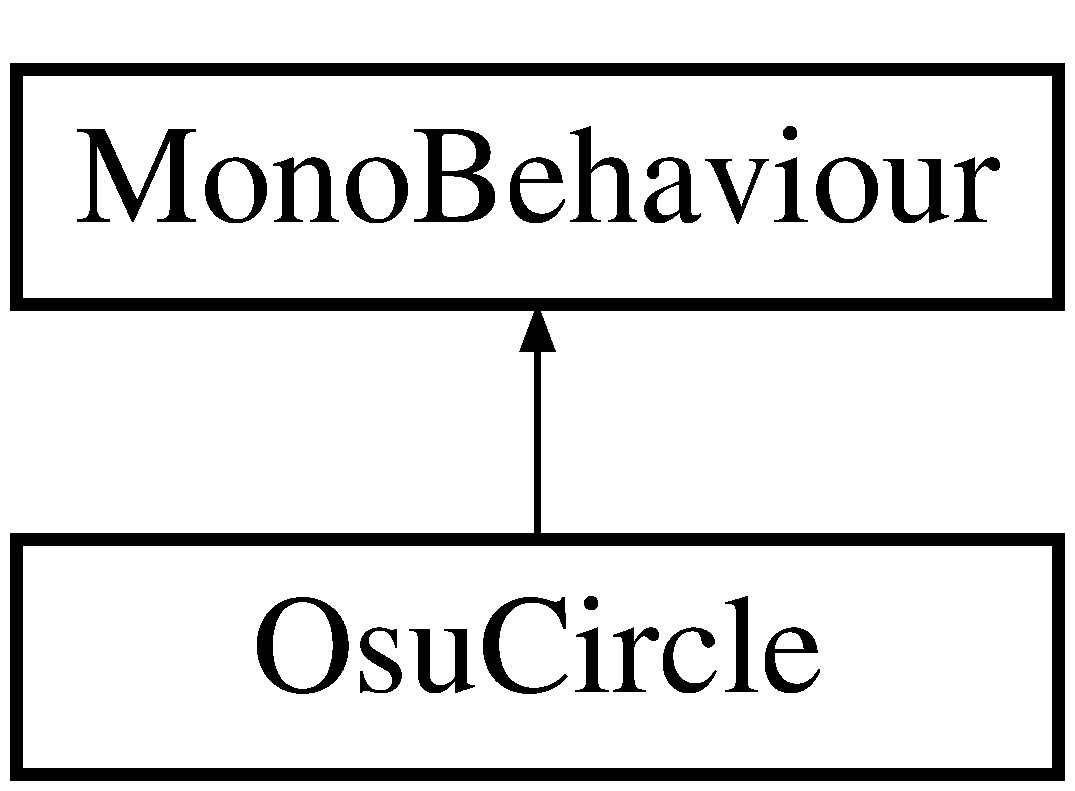
\includegraphics[height=2.000000cm]{class_osu_circle}
\end{center}
\end{figure}
\subsection*{Public Types}
\begin{DoxyCompactItemize}
\item 
\mbox{\Hypertarget{class_osu_circle_af50d7f27362dacb1dc3b3825cee7f837}\label{class_osu_circle_af50d7f27362dacb1dc3b3825cee7f837}} 
enum \hyperlink{class_osu_circle_af50d7f27362dacb1dc3b3825cee7f837}{arrow\+Types} \{ \newline
{\bfseries basic} = 0, 
{\bfseries fast} = 1, 
{\bfseries delayed} = 2, 
{\bfseries fire} = 3, 
\newline
{\bfseries ice} = 4, 
{\bfseries slow} = 5
 \}\begin{DoxyCompactList}\small\item\em $<$ Types of possible arrow types \end{DoxyCompactList}
\end{DoxyCompactItemize}
\subsection*{Public Member Functions}
\begin{DoxyCompactItemize}
\item 
\mbox{\Hypertarget{class_osu_circle_a108fbacb0b9c0261fddddb8c4212f474}\label{class_osu_circle_a108fbacb0b9c0261fddddb8c4212f474}} 
void {\bfseries cluster} (int num\+\_\+of\+\_\+obj)
\item 
void \hyperlink{class_osu_circle_ac1bcc007ef49c6e9de959168eea7bca4}{Hit\+Circle} ()
\item 
void \hyperlink{class_osu_circle_ae655fb82998de93d7542cb77f3ad406b}{Exchange\+Arrow} ()
\end{DoxyCompactItemize}
\subsection*{Public Attributes}
\begin{DoxyCompactItemize}
\item 
float \hyperlink{class_osu_circle_aaf07a385b1c32a713145d07dbaf9c5d0}{collapse\+\_\+speed}
\begin{DoxyCompactList}\small\item\em Speed at which the Approach\+Circle collapses. \end{DoxyCompactList}\item 
\mbox{\Hypertarget{class_osu_circle_abc723e35c4cd1c869fed1f2be58711fa}\label{class_osu_circle_abc723e35c4cd1c869fed1f2be58711fa}} 
Game\+Object \hyperlink{class_osu_circle_abc723e35c4cd1c869fed1f2be58711fa}{Arrow}
\begin{DoxyCompactList}\small\item\em Type of arrow associated with the \hyperlink{class_osu_circle}{Osu\+Circle}. \end{DoxyCompactList}\item 
\mbox{\Hypertarget{class_osu_circle_abf7710df78d144e2bbbf2ee514ba1f02}\label{class_osu_circle_abf7710df78d144e2bbbf2ee514ba1f02}} 
\hyperlink{class_osu_circle_af50d7f27362dacb1dc3b3825cee7f837}{arrow\+Types} \hyperlink{class_osu_circle_abf7710df78d144e2bbbf2ee514ba1f02}{arrow\+Type}
\begin{DoxyCompactList}\small\item\em \hyperlink{class_arrow}{Arrow} type holder. \end{DoxyCompactList}\item 
\mbox{\Hypertarget{class_osu_circle_a9fe96e2fefe4e4bb189bbd6d276aeb34}\label{class_osu_circle_a9fe96e2fefe4e4bb189bbd6d276aeb34}} 
float \hyperlink{class_osu_circle_a9fe96e2fefe4e4bb189bbd6d276aeb34}{Time\+Delay}
\begin{DoxyCompactList}\small\item\em Time to hit the circle. \end{DoxyCompactList}\item 
\mbox{\Hypertarget{class_osu_circle_a8e9ec841a5fbf5928ea676f1ba89a5e8}\label{class_osu_circle_a8e9ec841a5fbf5928ea676f1ba89a5e8}} 
float \hyperlink{class_osu_circle_a8e9ec841a5fbf5928ea676f1ba89a5e8}{approach\+Distance}
\begin{DoxyCompactList}\small\item\em Distance the Approach circle starts at. \end{DoxyCompactList}\item 
\mbox{\Hypertarget{class_osu_circle_a8f6408f9a87cff6a4297f129fb5f3920}\label{class_osu_circle_a8f6408f9a87cff6a4297f129fb5f3920}} 
bool \hyperlink{class_osu_circle_a8f6408f9a87cff6a4297f129fb5f3920}{hit}
\begin{DoxyCompactList}\small\item\em Bool handler wheather the button had beeen clicked. \end{DoxyCompactList}\item 
\mbox{\Hypertarget{class_osu_circle_a920d959e390a0e4a2e04c981aa608878}\label{class_osu_circle_a920d959e390a0e4a2e04c981aa608878}} 
Audio\+Source \hyperlink{class_osu_circle_a920d959e390a0e4a2e04c981aa608878}{source}
\begin{DoxyCompactList}\small\item\em Audio Source. \end{DoxyCompactList}\end{DoxyCompactItemize}
\subsection*{Private Member Functions}
\begin{DoxyCompactItemize}
\item 
void \hyperlink{class_osu_circle_ad681160a65a26c66917d2264c3a4d23c}{Start} ()
\item 
void \hyperlink{class_osu_circle_afe2813ce3da745f0e5a43aafad6fb419}{Update} ()
\item 
\mbox{\Hypertarget{class_osu_circle_a0aa9d1bda97523ca244fdd683d20b088}\label{class_osu_circle_a0aa9d1bda97523ca244fdd683d20b088}} 
void {\bfseries Late\+Update} ()
\end{DoxyCompactItemize}
\subsection*{Private Attributes}
\begin{DoxyCompactItemize}
\item 
\mbox{\Hypertarget{class_osu_circle_aab3f795104cc3e0e96b533dc8d627bc6}\label{class_osu_circle_aab3f795104cc3e0e96b533dc8d627bc6}} 
float \hyperlink{class_osu_circle_aab3f795104cc3e0e96b533dc8d627bc6}{Perfect\+Hit\+Time}
\begin{DoxyCompactList}\small\item\em Time trime value. \end{DoxyCompactList}\item 
\mbox{\Hypertarget{class_osu_circle_ae1fc5ef284ed08000b50578259e69fc1}\label{class_osu_circle_ae1fc5ef284ed08000b50578259e69fc1}} 
float \hyperlink{class_osu_circle_ae1fc5ef284ed08000b50578259e69fc1}{hit\+Score}
\begin{DoxyCompactList}\small\item\em Holds the score that the player hit the circle with. \end{DoxyCompactList}\item 
\mbox{\Hypertarget{class_osu_circle_aef5efb08c5ea74bd6875fda9456cd7d0}\label{class_osu_circle_aef5efb08c5ea74bd6875fda9456cd7d0}} 
Rect\+Transform \hyperlink{class_osu_circle_aef5efb08c5ea74bd6875fda9456cd7d0}{Approach\+Circle}
\begin{DoxyCompactList}\small\item\em Approach\+Cricle\textquotesingle{}s Position handled in later functions. \end{DoxyCompactList}\item 
\mbox{\Hypertarget{class_osu_circle_a6770527fce5f357a3d4a25ff68bf64a4}\label{class_osu_circle_a6770527fce5f357a3d4a25ff68bf64a4}} 
float \hyperlink{class_osu_circle_a6770527fce5f357a3d4a25ff68bf64a4}{Approach\+Rate}
\begin{DoxyCompactList}\small\item\em Defined rate of the aproach Cricle. \end{DoxyCompactList}\end{DoxyCompactItemize}


\subsection{Member Function Documentation}
\mbox{\Hypertarget{class_osu_circle_ae655fb82998de93d7542cb77f3ad406b}\label{class_osu_circle_ae655fb82998de93d7542cb77f3ad406b}} 
\index{Osu\+Circle@{Osu\+Circle}!Exchange\+Arrow@{Exchange\+Arrow}}
\index{Exchange\+Arrow@{Exchange\+Arrow}!Osu\+Circle@{Osu\+Circle}}
\subsubsection{\texorpdfstring{Exchange\+Arrow()}{ExchangeArrow()}}
{\footnotesize\ttfamily void Osu\+Circle.\+Exchange\+Arrow (\begin{DoxyParamCaption}{ }\end{DoxyParamCaption})}

Changes the arrow in the \hyperlink{class_spell_controller}{Spell\+Controller} to the new arrow that has just been hit. \mbox{\Hypertarget{class_osu_circle_ac1bcc007ef49c6e9de959168eea7bca4}\label{class_osu_circle_ac1bcc007ef49c6e9de959168eea7bca4}} 
\index{Osu\+Circle@{Osu\+Circle}!Hit\+Circle@{Hit\+Circle}}
\index{Hit\+Circle@{Hit\+Circle}!Osu\+Circle@{Osu\+Circle}}
\subsubsection{\texorpdfstring{Hit\+Circle()}{HitCircle()}}
{\footnotesize\ttfamily void Osu\+Circle.\+Hit\+Circle (\begin{DoxyParamCaption}{ }\end{DoxyParamCaption})}

Called when a Circle is hit in time \mbox{\Hypertarget{class_osu_circle_ad681160a65a26c66917d2264c3a4d23c}\label{class_osu_circle_ad681160a65a26c66917d2264c3a4d23c}} 
\index{Osu\+Circle@{Osu\+Circle}!Start@{Start}}
\index{Start@{Start}!Osu\+Circle@{Osu\+Circle}}
\subsubsection{\texorpdfstring{Start()}{Start()}}
{\footnotesize\ttfamily void Osu\+Circle.\+Start (\begin{DoxyParamCaption}{ }\end{DoxyParamCaption})\hspace{0.3cm}{\ttfamily [private]}}

Instantiates Member values \mbox{\Hypertarget{class_osu_circle_afe2813ce3da745f0e5a43aafad6fb419}\label{class_osu_circle_afe2813ce3da745f0e5a43aafad6fb419}} 
\index{Osu\+Circle@{Osu\+Circle}!Update@{Update}}
\index{Update@{Update}!Osu\+Circle@{Osu\+Circle}}
\subsubsection{\texorpdfstring{Update()}{Update()}}
{\footnotesize\ttfamily void Osu\+Circle.\+Update (\begin{DoxyParamCaption}{ }\end{DoxyParamCaption})\hspace{0.3cm}{\ttfamily [private]}}

updates \hyperlink{class_osu_circle}{Osu\+Circle} gameobject to check if it has been hit, or is pased its expected lifetime 

\subsection{Member Data Documentation}
\mbox{\Hypertarget{class_osu_circle_aaf07a385b1c32a713145d07dbaf9c5d0}\label{class_osu_circle_aaf07a385b1c32a713145d07dbaf9c5d0}} 
\index{Osu\+Circle@{Osu\+Circle}!collapse\+\_\+speed@{collapse\+\_\+speed}}
\index{collapse\+\_\+speed@{collapse\+\_\+speed}!Osu\+Circle@{Osu\+Circle}}
\subsubsection{\texorpdfstring{collapse\+\_\+speed}{collapse\_speed}}
{\footnotesize\ttfamily float Osu\+Circle.\+collapse\+\_\+speed}



Speed at which the Approach\+Circle collapses. 

Handles \hyperlink{class_osu_circle}{Osu\+Circle} objects that get instantiated on holding down fire 

The documentation for this class was generated from the following file\+:\begin{DoxyCompactItemize}
\item 
Assets/\+Scripts/\+U\+I/\+Osu/Osu\+Circle.\+cs\end{DoxyCompactItemize}

\hypertarget{class_pause_menu}{}\section{Pause\+Menu Class Reference}
\label{class_pause_menu}\index{Pause\+Menu@{Pause\+Menu}}
Inheritance diagram for Pause\+Menu\+:\begin{figure}[H]
\begin{center}
\leavevmode
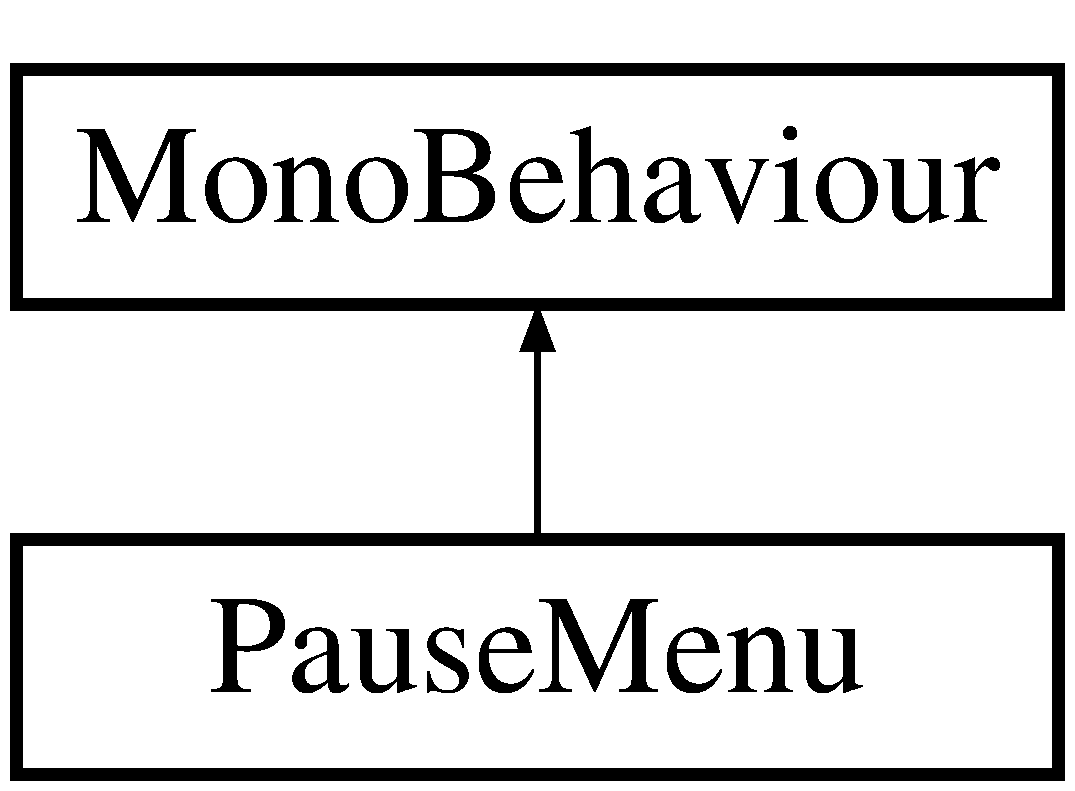
\includegraphics[height=2.000000cm]{class_pause_menu}
\end{center}
\end{figure}
\subsection*{Public Attributes}
\begin{DoxyCompactItemize}
\item 
\mbox{\Hypertarget{class_pause_menu_a52028e686cd9c745d5578a9ab6c22611}\label{class_pause_menu_a52028e686cd9c745d5578a9ab6c22611}} 
\hyperlink{class_game_controller}{Game\+Controller} \hyperlink{class_pause_menu_a52028e686cd9c745d5578a9ab6c22611}{GC}
\begin{DoxyCompactList}\small\item\em \hyperlink{class_game_controller}{Game\+Controller} object. \end{DoxyCompactList}\end{DoxyCompactItemize}
\subsection*{Private Member Functions}
\begin{DoxyCompactItemize}
\item 
void \hyperlink{class_pause_menu_ad66a0552c131257182ce524f1c71ce4c}{Update} ()
\end{DoxyCompactItemize}


\subsection{Detailed Description}
Handles the pause button and toggles the \hyperlink{class_game_controller}{Game\+Controller} 

\subsection{Member Function Documentation}
\mbox{\Hypertarget{class_pause_menu_ad66a0552c131257182ce524f1c71ce4c}\label{class_pause_menu_ad66a0552c131257182ce524f1c71ce4c}} 
\index{Pause\+Menu@{Pause\+Menu}!Update@{Update}}
\index{Update@{Update}!Pause\+Menu@{Pause\+Menu}}
\subsubsection{\texorpdfstring{Update()}{Update()}}
{\footnotesize\ttfamily void Pause\+Menu.\+Update (\begin{DoxyParamCaption}{ }\end{DoxyParamCaption})\hspace{0.3cm}{\ttfamily [private]}}

if espace is pressed, the gamecontroller will pause the game with \char`\"{}\+Toggle\+Pause\+Menu\char`\"{} 

The documentation for this class was generated from the following file\+:\begin{DoxyCompactItemize}
\item 
Assets/\+Scripts/\+U\+I/\+Menu/Pause\+Menu.\+cs\end{DoxyCompactItemize}

\hypertarget{class_pickup}{}\section{Pickup Class Reference}
\label{class_pickup}\index{Pickup@{Pickup}}
Inheritance diagram for Pickup\+:\begin{figure}[H]
\begin{center}
\leavevmode
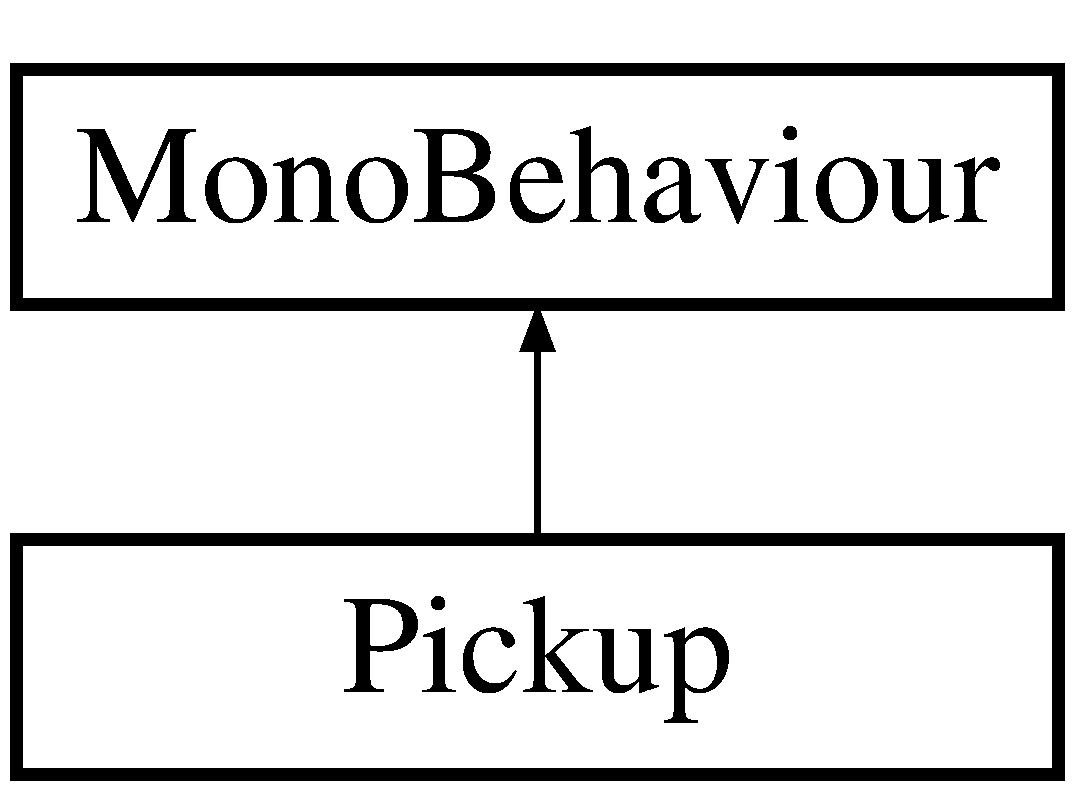
\includegraphics[height=2.000000cm]{class_pickup}
\end{center}
\end{figure}
\subsection*{Public Attributes}
\begin{DoxyCompactItemize}
\item 
\mbox{\Hypertarget{class_pickup_afcd81d084c606c839108b1226233e41b}\label{class_pickup_afcd81d084c606c839108b1226233e41b}} 
float \hyperlink{class_pickup_afcd81d084c606c839108b1226233e41b}{min\+Val} = 1.\+1f
\begin{DoxyCompactList}\small\item\em value the object adds lower bound \end{DoxyCompactList}\item 
\mbox{\Hypertarget{class_pickup_ab39a6532ea97da7e79051eed4414af28}\label{class_pickup_ab39a6532ea97da7e79051eed4414af28}} 
float \hyperlink{class_pickup_ab39a6532ea97da7e79051eed4414af28}{max\+Val} = 1.\+4f
\begin{DoxyCompactList}\small\item\em Value the object adds upper bound. \end{DoxyCompactList}\item 
\mbox{\Hypertarget{class_pickup_a0154f246e4265336bb743a19dcabf224}\label{class_pickup_a0154f246e4265336bb743a19dcabf224}} 
bool \hyperlink{class_pickup_a0154f246e4265336bb743a19dcabf224}{random\+Type}
\begin{DoxyCompactList}\small\item\em type of buff \end{DoxyCompactList}\item 
\mbox{\Hypertarget{class_pickup_a06a0397d6124a8cd3f35f14d20c36418}\label{class_pickup_a06a0397d6124a8cd3f35f14d20c36418}} 
bool {\bfseries random\+Val} = true
\item 
\mbox{\Hypertarget{class_pickup_a5dac153e6d3fc34709b91fc178bdbbbd}\label{class_pickup_a5dac153e6d3fc34709b91fc178bdbbbd}} 
pickup\+Types \hyperlink{class_pickup_a5dac153e6d3fc34709b91fc178bdbbbd}{pickup\+Type}
\begin{DoxyCompactList}\small\item\em the set pickup buff \end{DoxyCompactList}\item 
\mbox{\Hypertarget{class_pickup_a6d7b202bd29f9c620c8d2d266318e519}\label{class_pickup_a6d7b202bd29f9c620c8d2d266318e519}} 
float \hyperlink{class_pickup_a6d7b202bd29f9c620c8d2d266318e519}{pickup\+Value\+Or\+Mult} = 1f
\begin{DoxyCompactList}\small\item\em value or multiplier for pickup to apply to player \end{DoxyCompactList}\end{DoxyCompactItemize}
\subsection*{Private Member Functions}
\begin{DoxyCompactItemize}
\item 
void \hyperlink{class_pickup_aa0f4313f4bb636d95ec9ba901f4dc932}{Start} ()
\item 
void \hyperlink{class_pickup_a86ae9269c20eca5a07f9e6ae24eaae7c}{Fixed\+Update} ()
\item 
void \hyperlink{class_pickup_af91a544b99c9d52864ec6a074df98d73}{On\+Collision\+Enter} (Collision col)
\item 
void \hyperlink{class_pickup_a5f190e230de9ed4839c26642785896be}{On\+Trigger\+Enter} (Collider col)
\item 
void \hyperlink{class_pickup_a0375f0d9e0a3021b0718e565978498b0}{Use\+Effect} ()
\end{DoxyCompactItemize}
\subsection*{Private Attributes}
\begin{DoxyCompactItemize}
\item 
\mbox{\Hypertarget{class_pickup_a65bec7d3f99a526334f3d8e262b9f658}\label{class_pickup_a65bec7d3f99a526334f3d8e262b9f658}} 
\hyperlink{class_player}{Player} \hyperlink{class_pickup_a65bec7d3f99a526334f3d8e262b9f658}{player}
\begin{DoxyCompactList}\small\item\em \hyperlink{class_player}{Player} object. \end{DoxyCompactList}\end{DoxyCompactItemize}


\subsection{Member Function Documentation}
\mbox{\Hypertarget{class_pickup_a86ae9269c20eca5a07f9e6ae24eaae7c}\label{class_pickup_a86ae9269c20eca5a07f9e6ae24eaae7c}} 
\index{Pickup@{Pickup}!Fixed\+Update@{Fixed\+Update}}
\index{Fixed\+Update@{Fixed\+Update}!Pickup@{Pickup}}
\subsubsection{\texorpdfstring{Fixed\+Update()}{FixedUpdate()}}
{\footnotesize\ttfamily void Pickup.\+Fixed\+Update (\begin{DoxyParamCaption}{ }\end{DoxyParamCaption})\hspace{0.3cm}{\ttfamily [private]}}

slowly rotates the object \mbox{\Hypertarget{class_pickup_af91a544b99c9d52864ec6a074df98d73}\label{class_pickup_af91a544b99c9d52864ec6a074df98d73}} 
\index{Pickup@{Pickup}!On\+Collision\+Enter@{On\+Collision\+Enter}}
\index{On\+Collision\+Enter@{On\+Collision\+Enter}!Pickup@{Pickup}}
\subsubsection{\texorpdfstring{On\+Collision\+Enter()}{OnCollisionEnter()}}
{\footnotesize\ttfamily void Pickup.\+On\+Collision\+Enter (\begin{DoxyParamCaption}\item[{Collision}]{col }\end{DoxyParamCaption})\hspace{0.3cm}{\ttfamily [private]}}

Handels collision events, once it collides with the ground the Rigidbody should be set to Kinematic and not move 
\begin{DoxyParams}{Parameters}
{\em col} & is the oppisite collider \\
\hline
\end{DoxyParams}
\mbox{\Hypertarget{class_pickup_a5f190e230de9ed4839c26642785896be}\label{class_pickup_a5f190e230de9ed4839c26642785896be}} 
\index{Pickup@{Pickup}!On\+Trigger\+Enter@{On\+Trigger\+Enter}}
\index{On\+Trigger\+Enter@{On\+Trigger\+Enter}!Pickup@{Pickup}}
\subsubsection{\texorpdfstring{On\+Trigger\+Enter()}{OnTriggerEnter()}}
{\footnotesize\ttfamily void Pickup.\+On\+Trigger\+Enter (\begin{DoxyParamCaption}\item[{Collider}]{col }\end{DoxyParamCaption})\hspace{0.3cm}{\ttfamily [private]}}

Handels collision events where an object walks \char`\"{}into\char`\"{} the collider If the collider is the player, the player will pick up the item 
\begin{DoxyParams}{Parameters}
{\em col} & is the coliding object\textquotesingle{}s collider \\
\hline
\end{DoxyParams}
\mbox{\Hypertarget{class_pickup_aa0f4313f4bb636d95ec9ba901f4dc932}\label{class_pickup_aa0f4313f4bb636d95ec9ba901f4dc932}} 
\index{Pickup@{Pickup}!Start@{Start}}
\index{Start@{Start}!Pickup@{Pickup}}
\subsubsection{\texorpdfstring{Start()}{Start()}}
{\footnotesize\ttfamily void Pickup.\+Start (\begin{DoxyParamCaption}{ }\end{DoxyParamCaption})\hspace{0.3cm}{\ttfamily [private]}}

Instantiates member values and assigns pickup type (randomly) \mbox{\Hypertarget{class_pickup_a0375f0d9e0a3021b0718e565978498b0}\label{class_pickup_a0375f0d9e0a3021b0718e565978498b0}} 
\index{Pickup@{Pickup}!Use\+Effect@{Use\+Effect}}
\index{Use\+Effect@{Use\+Effect}!Pickup@{Pickup}}
\subsubsection{\texorpdfstring{Use\+Effect()}{UseEffect()}}
{\footnotesize\ttfamily void Pickup.\+Use\+Effect (\begin{DoxyParamCaption}{ }\end{DoxyParamCaption})\hspace{0.3cm}{\ttfamily [private]}}

handels how different types of pickups are set 

The documentation for this class was generated from the following file\+:\begin{DoxyCompactItemize}
\item 
Assets/\+Scripts/\+Entities/Pickup.\+cs\end{DoxyCompactItemize}

\hypertarget{class_player}{}\section{Player Class Reference}
\label{class_player}\index{Player@{Player}}
Inheritance diagram for Player\+:\begin{figure}[H]
\begin{center}
\leavevmode
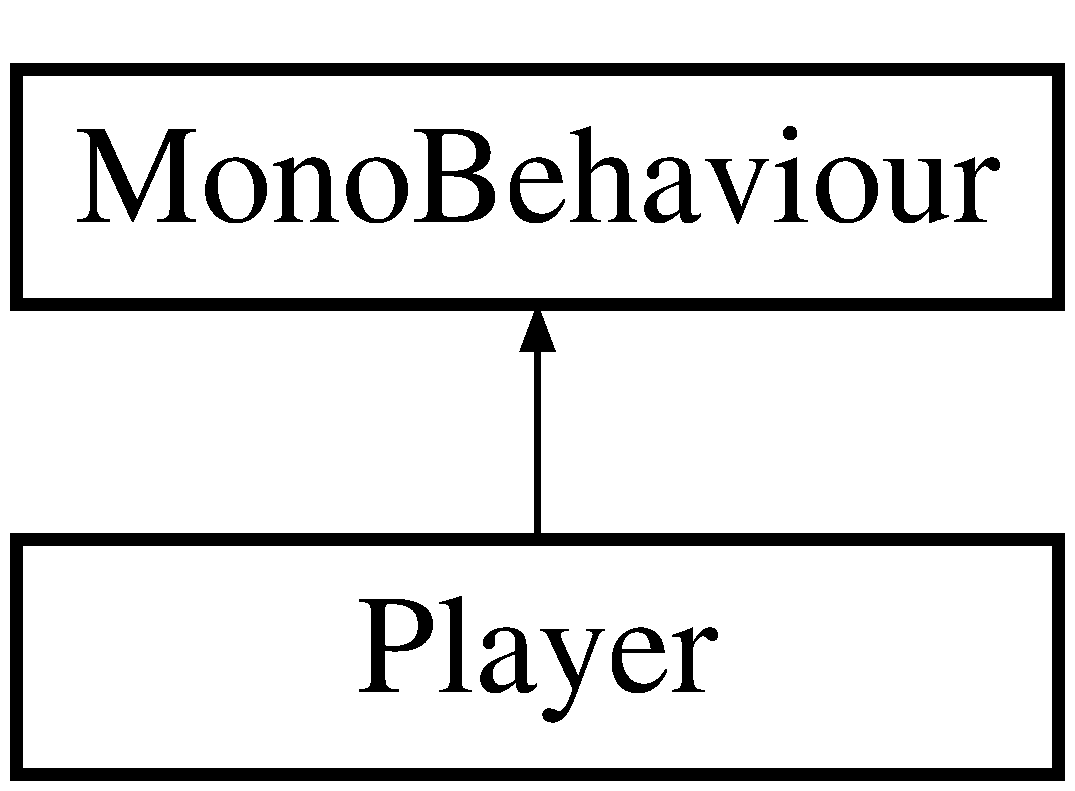
\includegraphics[height=2.000000cm]{class_player}
\end{center}
\end{figure}
\subsection*{Public Attributes}
\begin{DoxyCompactItemize}
\item 
\mbox{\Hypertarget{class_player_ac51bc0232fa16f956acee68e1635f7dc}\label{class_player_ac51bc0232fa16f956acee68e1635f7dc}} 
int \hyperlink{class_player_ac51bc0232fa16f956acee68e1635f7dc}{max\+Health} = 5
\begin{DoxyCompactList}\small\item\em Maxhealth of the player. \end{DoxyCompactList}\item 
\mbox{\Hypertarget{class_player_ab064f330cef84e2e062fd6446db24184}\label{class_player_ab064f330cef84e2e062fd6446db24184}} 
int \hyperlink{class_player_ab064f330cef84e2e062fd6446db24184}{health} = 5
\begin{DoxyCompactList}\small\item\em Current health that gets changed. \end{DoxyCompactList}\item 
\mbox{\Hypertarget{class_player_abd2291a934964b32e9bc06a7738042d3}\label{class_player_abd2291a934964b32e9bc06a7738042d3}} 
float \hyperlink{class_player_abd2291a934964b32e9bc06a7738042d3}{speed} = 5.\+0f
\begin{DoxyCompactList}\small\item\em Starting speed of the player. \end{DoxyCompactList}\item 
\mbox{\Hypertarget{class_player_a28b98e6712f03b881b07792d3c457f65}\label{class_player_a28b98e6712f03b881b07792d3c457f65}} 
float \hyperlink{class_player_a28b98e6712f03b881b07792d3c457f65}{rotation\+Speed}
\begin{DoxyCompactList}\small\item\em rotational speed of the player \end{DoxyCompactList}\item 
\mbox{\Hypertarget{class_player_ad71f4fd6a20074d500df63092298de62}\label{class_player_ad71f4fd6a20074d500df63092298de62}} 
float \hyperlink{class_player_ad71f4fd6a20074d500df63092298de62}{arrow\+Speed} = 40f
\begin{DoxyCompactList}\small\item\em How fast arrows are initially shot at. \end{DoxyCompactList}\item 
\mbox{\Hypertarget{class_player_aecc56aacf8bc7000018ee06406a60076}\label{class_player_aecc56aacf8bc7000018ee06406a60076}} 
float \hyperlink{class_player_aecc56aacf8bc7000018ee06406a60076}{arrow\+Dmg} = 5f
\begin{DoxyCompactList}\small\item\em How much damage arrows initially do. \end{DoxyCompactList}\item 
\mbox{\Hypertarget{class_player_ab8d9c5f386d98a1b32ccc928f8d4d29b}\label{class_player_ab8d9c5f386d98a1b32ccc928f8d4d29b}} 
int \hyperlink{class_player_ab8d9c5f386d98a1b32ccc928f8d4d29b}{burn\+Amount} = 5
\begin{DoxyCompactList}\small\item\em Default \char`\"{}burn\char`\"{} damage for fire arrows. \end{DoxyCompactList}\item 
\mbox{\Hypertarget{class_player_a1723357f7c7ee28c6fe9d366708e83e8}\label{class_player_a1723357f7c7ee28c6fe9d366708e83e8}} 
float \hyperlink{class_player_a1723357f7c7ee28c6fe9d366708e83e8}{freeze\+Time} = 2f
\begin{DoxyCompactList}\small\item\em default \char`\"{}\+Freeze\char`\"{} time for ice arrows \end{DoxyCompactList}\item 
\mbox{\Hypertarget{class_player_a17b09d930d828bb77903afa04073c3b2}\label{class_player_a17b09d930d828bb77903afa04073c3b2}} 
float \hyperlink{class_player_a17b09d930d828bb77903afa04073c3b2}{slow\+Mult} = 1.\+5f
\begin{DoxyCompactList}\small\item\em Default speed multiplier for slow arrows. \end{DoxyCompactList}\item 
\mbox{\Hypertarget{class_player_a98d070bc739f23a42d48d3eae30badd0}\label{class_player_a98d070bc739f23a42d48d3eae30badd0}} 
Texture2D \hyperlink{class_player_a98d070bc739f23a42d48d3eae30badd0}{Hp\+Bar\+Texture}
\begin{DoxyCompactList}\small\item\em Texture for player healthbar. \end{DoxyCompactList}\item 
\mbox{\Hypertarget{class_player_a91d04489f1b738260a27fba902157f9b}\label{class_player_a91d04489f1b738260a27fba902157f9b}} 
Texture2D \hyperlink{class_player_a91d04489f1b738260a27fba902157f9b}{Hp\+Back\+Texture}
\begin{DoxyCompactList}\small\item\em back texture for \hyperlink{class_player}{Player} health \end{DoxyCompactList}\end{DoxyCompactItemize}
\subsection*{Private Member Functions}
\begin{DoxyCompactItemize}
\item 
void \hyperlink{class_player_a1a09a3ded16ac1646f6bdd4f25fe0ddd}{Start} ()
\item 
void \hyperlink{class_player_aace80372e18e32fe177e295fe5d93ba8}{Update} ()
\item 
void \hyperlink{class_player_aa0458562e3da0655ecb39a0031114335}{Fixed\+Update} ()
\item 
void \hyperlink{class_player_abd430d273ef011a22a6c63eee5067751}{On\+Collision\+Enter} (Collision col)
\item 
void \hyperlink{class_player_a281fbfe9664d247f3e4d4b2911b00dbe}{On\+Collision\+Stay} (Collision col)
\item 
void \hyperlink{class_player_a65c37e862c41df23b43ffc646ffa9fd0}{Aim\+Player} ()
\item 
void \hyperlink{class_player_a8d9dc0cb892c8fdb15f25e41c7189ebd}{Movement} ()
\begin{DoxyCompactList}\small\item\em Test for Health Bar. \end{DoxyCompactList}\item 
\mbox{\Hypertarget{class_player_a37c8ce5286efb3918e92a26892a09b12}\label{class_player_a37c8ce5286efb3918e92a26892a09b12}} 
void \hyperlink{class_player_a37c8ce5286efb3918e92a26892a09b12}{On\+G\+UI} ()
\begin{DoxyCompactList}\small\item\em Undoes the invulnerablitiy of the player. \end{DoxyCompactList}\item 
\mbox{\Hypertarget{class_player_a368f95446e99f0f007014e5755d91777}\label{class_player_a368f95446e99f0f007014e5755d91777}} 
void {\bfseries Reset\+Vulnerability} ()
\end{DoxyCompactItemize}
\subsection*{Private Attributes}
\begin{DoxyCompactItemize}
\item 
\mbox{\Hypertarget{class_player_aab2a1e98356973545e45c3071190b8e5}\label{class_player_aab2a1e98356973545e45c3071190b8e5}} 
bool \hyperlink{class_player_aab2a1e98356973545e45c3071190b8e5}{invulnerable} = false
\begin{DoxyCompactList}\small\item\em Sets invulnerablility after player has taken damage. \end{DoxyCompactList}\item 
\mbox{\Hypertarget{class_player_a36830e22f302a4e03aa615efbc472881}\label{class_player_a36830e22f302a4e03aa615efbc472881}} 
Camera \hyperlink{class_player_a36830e22f302a4e03aa615efbc472881}{main\+Cam}
\begin{DoxyCompactList}\small\item\em main camera object \end{DoxyCompactList}\item 
\mbox{\Hypertarget{class_player_a5dfe4ae1b620a31044be3d8987a8661e}\label{class_player_a5dfe4ae1b620a31044be3d8987a8661e}} 
Ray \hyperlink{class_player_a5dfe4ae1b620a31044be3d8987a8661e}{cam\+Ray}
\begin{DoxyCompactList}\small\item\em Ray from camera to mouse position. \end{DoxyCompactList}\item 
\mbox{\Hypertarget{class_player_a896f013d0fa8988d8508aac39ecf676d}\label{class_player_a896f013d0fa8988d8508aac39ecf676d}} 
Raycast\+Hit \hyperlink{class_player_a896f013d0fa8988d8508aac39ecf676d}{cam\+Ray\+Hit}
\begin{DoxyCompactList}\small\item\em Hit point of raycast. \end{DoxyCompactList}\item 
\mbox{\Hypertarget{class_player_a2954d91cf05871fed826b707e65604c5}\label{class_player_a2954d91cf05871fed826b707e65604c5}} 
Vector3 \hyperlink{class_player_a2954d91cf05871fed826b707e65604c5}{deltamovement}
\begin{DoxyCompactList}\small\item\em Change in movement. \end{DoxyCompactList}\item 
\mbox{\Hypertarget{class_player_ae0baab096eb0714ffa516b6a1de9eed6}\label{class_player_ae0baab096eb0714ffa516b6a1de9eed6}} 
\hyperlink{class_game_controller}{Game\+Controller} \hyperlink{class_player_ae0baab096eb0714ffa516b6a1de9eed6}{gamecontroller}
\begin{DoxyCompactList}\small\item\em Gamecontroller object. \end{DoxyCompactList}\item 
\mbox{\Hypertarget{class_player_aa05f0fb4e449ec97d7bf20fd90aa1967}\label{class_player_aa05f0fb4e449ec97d7bf20fd90aa1967}} 
\hyperlink{class_spell_controller}{Spell\+Controller} \hyperlink{class_player_aa05f0fb4e449ec97d7bf20fd90aa1967}{spell\+UI}
\begin{DoxyCompactList}\small\item\em \hyperlink{class_spell_controller}{Spell\+Controller} object. \end{DoxyCompactList}\item 
\mbox{\Hypertarget{class_player_afb08071e4a3f39dc03d0f36fad786dab}\label{class_player_afb08071e4a3f39dc03d0f36fad786dab}} 
\hyperlink{class_u_i_controller}{U\+I\+Controller} \hyperlink{class_player_afb08071e4a3f39dc03d0f36fad786dab}{uic}
\begin{DoxyCompactList}\small\item\em UI Controller object. \end{DoxyCompactList}\item 
\mbox{\Hypertarget{class_player_ad5c386687ea25d8dc7ed86fdd0850608}\label{class_player_ad5c386687ea25d8dc7ed86fdd0850608}} 
double \hyperlink{class_player_ad5c386687ea25d8dc7ed86fdd0850608}{time\+Held}
\begin{DoxyCompactList}\small\item\em Time holding fire. \end{DoxyCompactList}\item 
\mbox{\Hypertarget{class_player_a97f79d09dde65f96851c5b92d5db79b7}\label{class_player_a97f79d09dde65f96851c5b92d5db79b7}} 
double {\bfseries test}
\item 
\mbox{\Hypertarget{class_player_ad694265b88e8ce48081e240b9ec915f2}\label{class_player_ad694265b88e8ce48081e240b9ec915f2}} 
bool \hyperlink{class_player_ad694265b88e8ce48081e240b9ec915f2}{right\+Clicked}
\begin{DoxyCompactList}\small\item\em Bool for clicking the right mouse button. \end{DoxyCompactList}\item 
\mbox{\Hypertarget{class_player_acc2c43dd193b137522c1ad100fff0822}\label{class_player_acc2c43dd193b137522c1ad100fff0822}} 
float \hyperlink{class_player_acc2c43dd193b137522c1ad100fff0822}{speed\+After\+Pause}
\begin{DoxyCompactList}\small\item\em Pausing handling. \end{DoxyCompactList}\item 
\mbox{\Hypertarget{class_player_a49e75b5b68fa87751080bf40504fbdf3}\label{class_player_a49e75b5b68fa87751080bf40504fbdf3}} 
float \hyperlink{class_player_a49e75b5b68fa87751080bf40504fbdf3}{hp\+Bar\+Length}
\begin{DoxyCompactList}\small\item\em Length of healthbar. \end{DoxyCompactList}\item 
\mbox{\Hypertarget{class_player_a70b6b51d74cd56fa84d032a4024792e6}\label{class_player_a70b6b51d74cd56fa84d032a4024792e6}} 
Animator \hyperlink{class_player_a70b6b51d74cd56fa84d032a4024792e6}{anim}
\begin{DoxyCompactList}\small\item\em Animator controller. \end{DoxyCompactList}\end{DoxyCompactItemize}


\subsection{Detailed Description}
Everything player related is in this class 

\subsection{Member Function Documentation}
\mbox{\Hypertarget{class_player_a65c37e862c41df23b43ffc646ffa9fd0}\label{class_player_a65c37e862c41df23b43ffc646ffa9fd0}} 
\index{Player@{Player}!Aim\+Player@{Aim\+Player}}
\index{Aim\+Player@{Aim\+Player}!Player@{Player}}
\subsubsection{\texorpdfstring{Aim\+Player()}{AimPlayer()}}
{\footnotesize\ttfamily void Player.\+Aim\+Player (\begin{DoxyParamCaption}{ }\end{DoxyParamCaption})\hspace{0.3cm}{\ttfamily [private]}}

Aims player at the position the Mouse casts onto the gameworld \mbox{\Hypertarget{class_player_aa0458562e3da0655ecb39a0031114335}\label{class_player_aa0458562e3da0655ecb39a0031114335}} 
\index{Player@{Player}!Fixed\+Update@{Fixed\+Update}}
\index{Fixed\+Update@{Fixed\+Update}!Player@{Player}}
\subsubsection{\texorpdfstring{Fixed\+Update()}{FixedUpdate()}}
{\footnotesize\ttfamily void Player.\+Fixed\+Update (\begin{DoxyParamCaption}{ }\end{DoxyParamCaption})\hspace{0.3cm}{\ttfamily [private]}}

Aim the player Polar the mouse\textquotesingle{}s current position on screen to the game world \mbox{\Hypertarget{class_player_a8d9dc0cb892c8fdb15f25e41c7189ebd}\label{class_player_a8d9dc0cb892c8fdb15f25e41c7189ebd}} 
\index{Player@{Player}!Movement@{Movement}}
\index{Movement@{Movement}!Player@{Player}}
\subsubsection{\texorpdfstring{Movement()}{Movement()}}
{\footnotesize\ttfamily void Player.\+Movement (\begin{DoxyParamCaption}{ }\end{DoxyParamCaption})\hspace{0.3cm}{\ttfamily [private]}}



Test for Health Bar. 

Handles movement of the player in the gameworld with key interactiosn and Unitys Simple\+Movement class \mbox{\Hypertarget{class_player_abd430d273ef011a22a6c63eee5067751}\label{class_player_abd430d273ef011a22a6c63eee5067751}} 
\index{Player@{Player}!On\+Collision\+Enter@{On\+Collision\+Enter}}
\index{On\+Collision\+Enter@{On\+Collision\+Enter}!Player@{Player}}
\subsubsection{\texorpdfstring{On\+Collision\+Enter()}{OnCollisionEnter()}}
{\footnotesize\ttfamily void Player.\+On\+Collision\+Enter (\begin{DoxyParamCaption}\item[{Collision}]{col }\end{DoxyParamCaption})\hspace{0.3cm}{\ttfamily [private]}}

Handels collision events \mbox{\Hypertarget{class_player_a281fbfe9664d247f3e4d4b2911b00dbe}\label{class_player_a281fbfe9664d247f3e4d4b2911b00dbe}} 
\index{Player@{Player}!On\+Collision\+Stay@{On\+Collision\+Stay}}
\index{On\+Collision\+Stay@{On\+Collision\+Stay}!Player@{Player}}
\subsubsection{\texorpdfstring{On\+Collision\+Stay()}{OnCollisionStay()}}
{\footnotesize\ttfamily void Player.\+On\+Collision\+Stay (\begin{DoxyParamCaption}\item[{Collision}]{col }\end{DoxyParamCaption})\hspace{0.3cm}{\ttfamily [private]}}

Handles how collisions interact when remaining inside the hitboxes of the player \mbox{\Hypertarget{class_player_a1a09a3ded16ac1646f6bdd4f25fe0ddd}\label{class_player_a1a09a3ded16ac1646f6bdd4f25fe0ddd}} 
\index{Player@{Player}!Start@{Start}}
\index{Start@{Start}!Player@{Player}}
\subsubsection{\texorpdfstring{Start()}{Start()}}
{\footnotesize\ttfamily void Player.\+Start (\begin{DoxyParamCaption}{ }\end{DoxyParamCaption})\hspace{0.3cm}{\ttfamily [private]}}

Instantiates member values \mbox{\Hypertarget{class_player_aace80372e18e32fe177e295fe5d93ba8}\label{class_player_aace80372e18e32fe177e295fe5d93ba8}} 
\index{Player@{Player}!Update@{Update}}
\index{Update@{Update}!Player@{Player}}
\subsubsection{\texorpdfstring{Update()}{Update()}}
{\footnotesize\ttfamily void Player.\+Update (\begin{DoxyParamCaption}{ }\end{DoxyParamCaption})\hspace{0.3cm}{\ttfamily [private]}}

Updates member valeus Health set to appropriate length Also handles basic inputs for walking animation 

The documentation for this class was generated from the following file\+:\begin{DoxyCompactItemize}
\item 
Assets/\+Scripts/\+Entities/Player.\+cs\end{DoxyCompactItemize}

\hypertarget{class_quit_on_click}{}\section{Quit\+On\+Click Class Reference}
\label{class_quit_on_click}\index{Quit\+On\+Click@{Quit\+On\+Click}}
Inheritance diagram for Quit\+On\+Click\+:\begin{figure}[H]
\begin{center}
\leavevmode
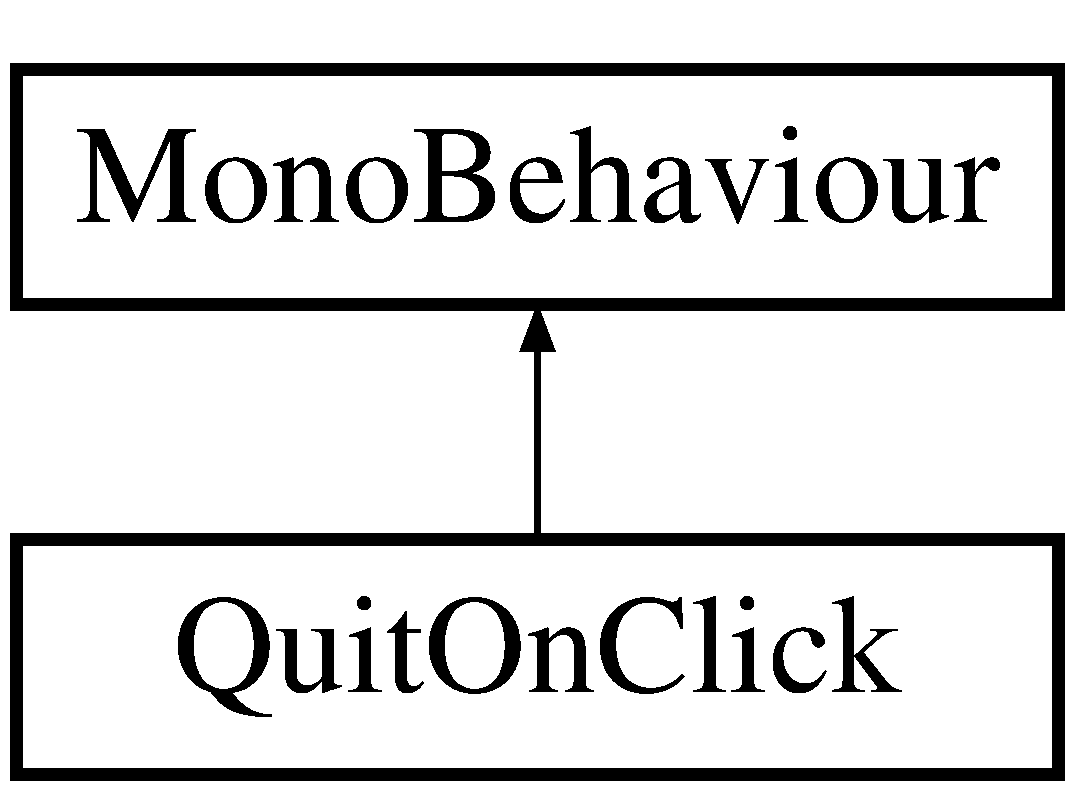
\includegraphics[height=2.000000cm]{class_quit_on_click}
\end{center}
\end{figure}
\subsection*{Public Member Functions}
\begin{DoxyCompactItemize}
\item 
void \hyperlink{class_quit_on_click_a2ae4a389fc44a04218d7a1353bcc870a}{Quit} ()
\end{DoxyCompactItemize}


\subsection{Detailed Description}
Handles how unity will quit the application 

\subsection{Member Function Documentation}
\mbox{\Hypertarget{class_quit_on_click_a2ae4a389fc44a04218d7a1353bcc870a}\label{class_quit_on_click_a2ae4a389fc44a04218d7a1353bcc870a}} 
\index{Quit\+On\+Click@{Quit\+On\+Click}!Quit@{Quit}}
\index{Quit@{Quit}!Quit\+On\+Click@{Quit\+On\+Click}}
\subsubsection{\texorpdfstring{Quit()}{Quit()}}
{\footnotesize\ttfamily void Quit\+On\+Click.\+Quit (\begin{DoxyParamCaption}{ }\end{DoxyParamCaption})}

Checks the application if its in editor, the changes how quiting the game runs \begin{DoxyNote}{Note}
Application.\+Quit() will not work inside editor, only build 
\end{DoxyNote}


The documentation for this class was generated from the following file\+:\begin{DoxyCompactItemize}
\item 
Assets/\+Scripts/\+U\+I/\+Menu/Quit\+On\+Click.\+cs\end{DoxyCompactItemize}

\hypertarget{class_scene_controller}{}\section{Scene\+Controller Class Reference}
\label{class_scene_controller}\index{Scene\+Controller@{Scene\+Controller}}
Inheritance diagram for Scene\+Controller\+:\begin{figure}[H]
\begin{center}
\leavevmode
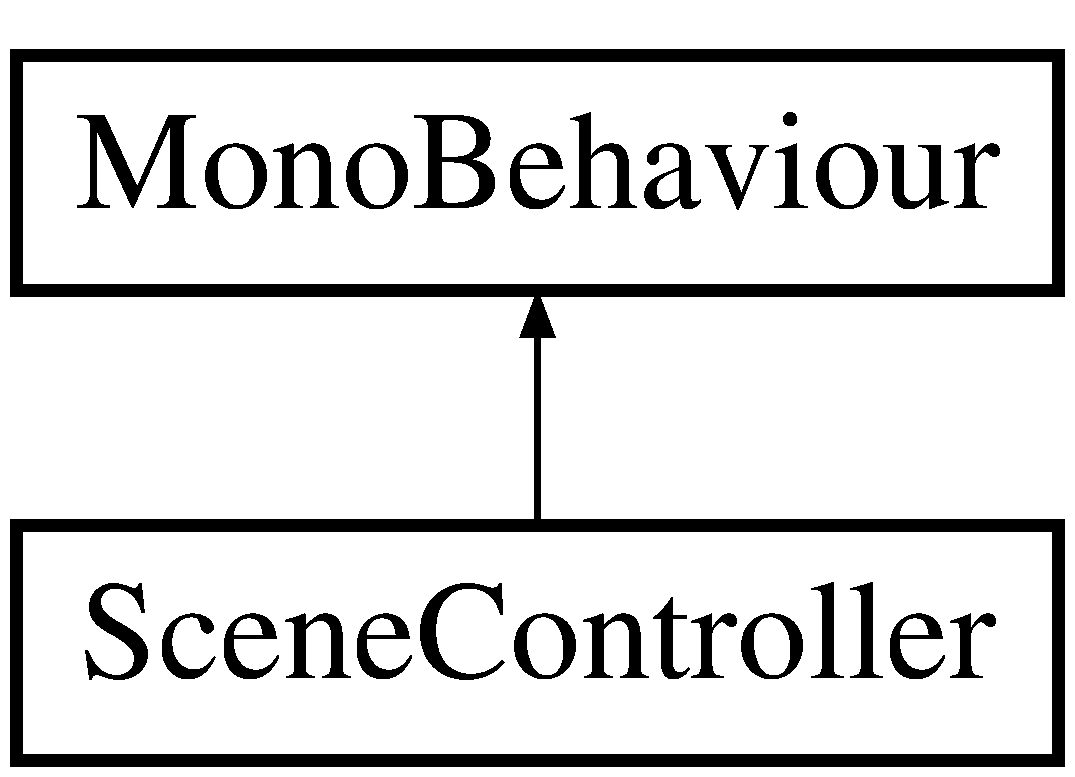
\includegraphics[height=2.000000cm]{class_scene_controller}
\end{center}
\end{figure}
\subsection*{Public Member Functions}
\begin{DoxyCompactItemize}
\item 
void \hyperlink{class_scene_controller_ab4c9c8564748875f4eb983c861783716}{Load\+Game} ()
\item 
void \hyperlink{class_scene_controller_a4fb5d32427ebae6e59dc136a3a15d07c}{Load\+Menu} ()
\item 
void \hyperlink{class_scene_controller_a9b24f2313df6b1ee47e72a978fc3528d}{Quit} ()
\end{DoxyCompactItemize}


\subsection{Detailed Description}
Handles menu interaction and global interactions 

\subsection{Member Function Documentation}
\mbox{\Hypertarget{class_scene_controller_ab4c9c8564748875f4eb983c861783716}\label{class_scene_controller_ab4c9c8564748875f4eb983c861783716}} 
\index{Scene\+Controller@{Scene\+Controller}!Load\+Game@{Load\+Game}}
\index{Load\+Game@{Load\+Game}!Scene\+Controller@{Scene\+Controller}}
\subsubsection{\texorpdfstring{Load\+Game()}{LoadGame()}}
{\footnotesize\ttfamily void Scene\+Controller.\+Load\+Game (\begin{DoxyParamCaption}{ }\end{DoxyParamCaption})}

Loads Testworld scene (with the game) \mbox{\Hypertarget{class_scene_controller_a4fb5d32427ebae6e59dc136a3a15d07c}\label{class_scene_controller_a4fb5d32427ebae6e59dc136a3a15d07c}} 
\index{Scene\+Controller@{Scene\+Controller}!Load\+Menu@{Load\+Menu}}
\index{Load\+Menu@{Load\+Menu}!Scene\+Controller@{Scene\+Controller}}
\subsubsection{\texorpdfstring{Load\+Menu()}{LoadMenu()}}
{\footnotesize\ttfamily void Scene\+Controller.\+Load\+Menu (\begin{DoxyParamCaption}{ }\end{DoxyParamCaption})}

Load main menu \mbox{\Hypertarget{class_scene_controller_a9b24f2313df6b1ee47e72a978fc3528d}\label{class_scene_controller_a9b24f2313df6b1ee47e72a978fc3528d}} 
\index{Scene\+Controller@{Scene\+Controller}!Quit@{Quit}}
\index{Quit@{Quit}!Scene\+Controller@{Scene\+Controller}}
\subsubsection{\texorpdfstring{Quit()}{Quit()}}
{\footnotesize\ttfamily void Scene\+Controller.\+Quit (\begin{DoxyParamCaption}{ }\end{DoxyParamCaption})}

When called, quits the application 

The documentation for this class was generated from the following file\+:\begin{DoxyCompactItemize}
\item 
Assets/\+Scripts/\+Controllers/Scene\+Controller.\+cs\end{DoxyCompactItemize}

\hypertarget{class_select_on_input}{}\section{Select\+On\+Input Class Reference}
\label{class_select_on_input}\index{Select\+On\+Input@{Select\+On\+Input}}
Inheritance diagram for Select\+On\+Input\+:\begin{figure}[H]
\begin{center}
\leavevmode
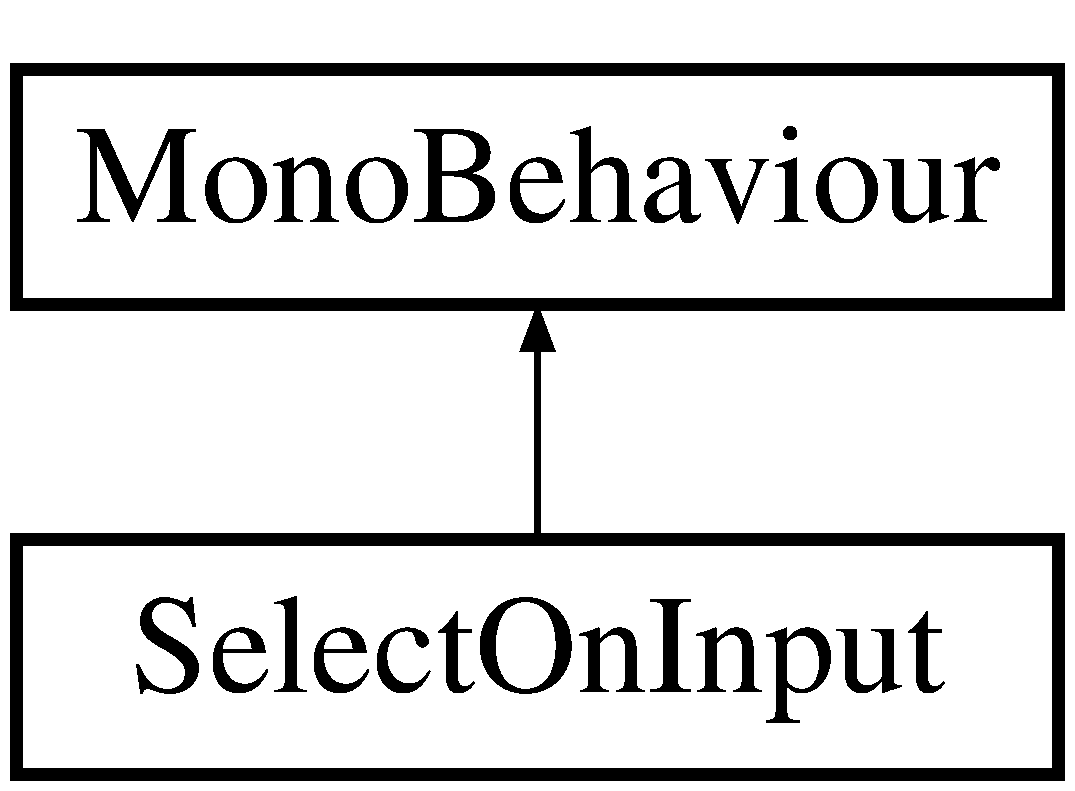
\includegraphics[height=2.000000cm]{class_select_on_input}
\end{center}
\end{figure}
\subsection*{Public Attributes}
\begin{DoxyCompactItemize}
\item 
\mbox{\Hypertarget{class_select_on_input_adf9cd7303f57e21b83a1d7f537158cc0}\label{class_select_on_input_adf9cd7303f57e21b83a1d7f537158cc0}} 
Event\+System \hyperlink{class_select_on_input_adf9cd7303f57e21b83a1d7f537158cc0}{event\+System}
\begin{DoxyCompactList}\small\item\em Unity Event\+System caller (used in menus) \end{DoxyCompactList}\item 
\mbox{\Hypertarget{class_select_on_input_a7c45b36a1cf3101337a96d6a2c18ff5c}\label{class_select_on_input_a7c45b36a1cf3101337a96d6a2c18ff5c}} 
Game\+Object \hyperlink{class_select_on_input_a7c45b36a1cf3101337a96d6a2c18ff5c}{selected\+Object}
\begin{DoxyCompactList}\small\item\em object that has been selected \end{DoxyCompactList}\end{DoxyCompactItemize}
\subsection*{Private Member Functions}
\begin{DoxyCompactItemize}
\item 
\mbox{\Hypertarget{class_select_on_input_a3ffd4bde4e9564050cbe707c8c75d17a}\label{class_select_on_input_a3ffd4bde4e9564050cbe707c8c75d17a}} 
void \hyperlink{class_select_on_input_a3ffd4bde4e9564050cbe707c8c75d17a}{Update} ()
\begin{DoxyCompactList}\small\item\em resets button\+Selected value \end{DoxyCompactList}\item 
\mbox{\Hypertarget{class_select_on_input_a091beca3bb995b8408358b1949d526aa}\label{class_select_on_input_a091beca3bb995b8408358b1949d526aa}} 
void {\bfseries On\+Disable} ()
\end{DoxyCompactItemize}
\subsection*{Private Attributes}
\begin{DoxyCompactItemize}
\item 
bool \hyperlink{class_select_on_input_a32ff6bfbb80619aed84e0e66ee1094ab}{button\+Selected}
\begin{DoxyCompactList}\small\item\em boolean handler for if a button has been selected \end{DoxyCompactList}\end{DoxyCompactItemize}


\subsection{Member Data Documentation}
\mbox{\Hypertarget{class_select_on_input_a32ff6bfbb80619aed84e0e66ee1094ab}\label{class_select_on_input_a32ff6bfbb80619aed84e0e66ee1094ab}} 
\index{Select\+On\+Input@{Select\+On\+Input}!button\+Selected@{button\+Selected}}
\index{button\+Selected@{button\+Selected}!Select\+On\+Input@{Select\+On\+Input}}
\subsubsection{\texorpdfstring{button\+Selected}{buttonSelected}}
{\footnotesize\ttfamily bool Select\+On\+Input.\+button\+Selected\hspace{0.3cm}{\ttfamily [private]}}



boolean handler for if a button has been selected 

updates for when buttons are clicked 

The documentation for this class was generated from the following file\+:\begin{DoxyCompactItemize}
\item 
Assets/\+Scripts/\+U\+I/\+Menu/Select\+On\+Input.\+cs\end{DoxyCompactItemize}

\hypertarget{class_shooting_aim_line}{}\section{Shooting\+Aim\+Line Class Reference}
\label{class_shooting_aim_line}\index{Shooting\+Aim\+Line@{Shooting\+Aim\+Line}}
Inheritance diagram for Shooting\+Aim\+Line\+:\begin{figure}[H]
\begin{center}
\leavevmode
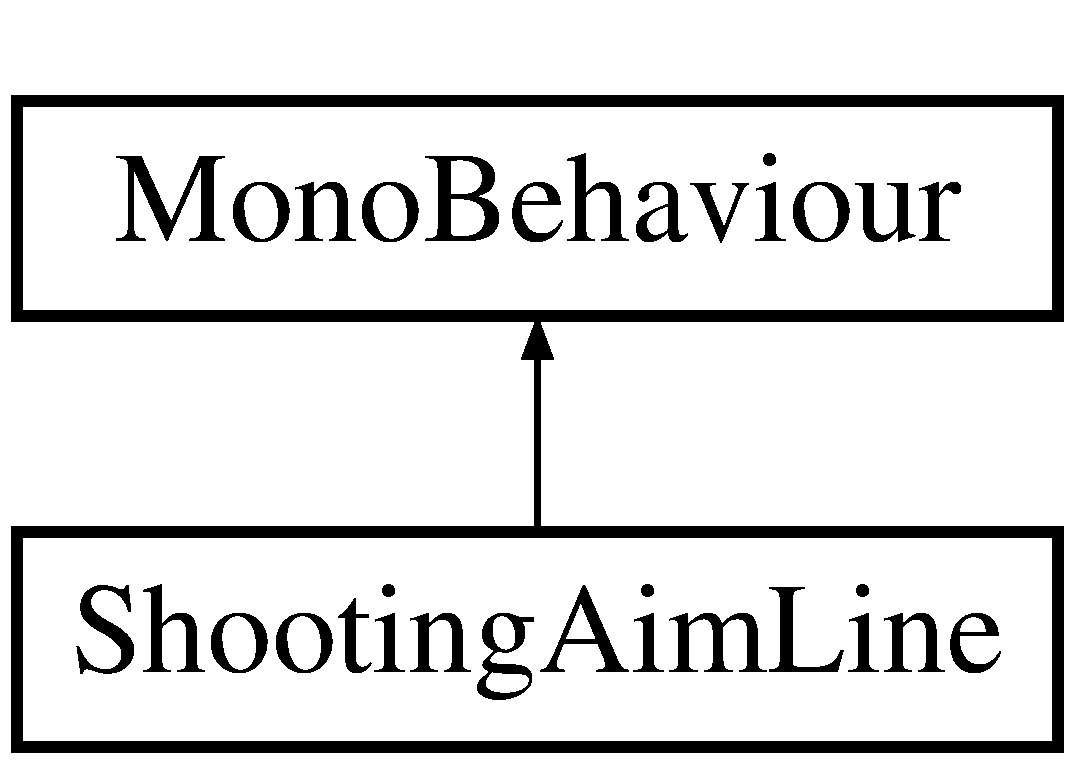
\includegraphics[height=2.000000cm]{class_shooting_aim_line}
\end{center}
\end{figure}
\subsection*{Private Member Functions}
\begin{DoxyCompactItemize}
\item 
void \hyperlink{class_shooting_aim_line_aea74f66ae5a79b70d07dbc7fe4970f34}{Start} ()
\item 
void \hyperlink{class_shooting_aim_line_abe1fb3aafc6c03c5010c842026b1368a}{Late\+Update} ()
\end{DoxyCompactItemize}
\subsection*{Private Attributes}
\begin{DoxyCompactItemize}
\item 
Camera \hyperlink{class_shooting_aim_line_a7198b2c13fc8ce0a388f82138362cd67}{main\+Cam}
\begin{DoxyCompactList}\small\item\em main\+Camera object \end{DoxyCompactList}\item 
\mbox{\Hypertarget{class_shooting_aim_line_a10ac775070726d01148aafc2471aab2a}\label{class_shooting_aim_line_a10ac775070726d01148aafc2471aab2a}} 
\hyperlink{class_spell_controller}{Spell\+Controller} \hyperlink{class_shooting_aim_line_a10ac775070726d01148aafc2471aab2a}{spell\+Controller}
\begin{DoxyCompactList}\small\item\em \hyperlink{class_spell_controller}{Spell\+Controller}. \end{DoxyCompactList}\item 
\mbox{\Hypertarget{class_shooting_aim_line_ae75dab10b6a07d162b97fe42d3c7075c}\label{class_shooting_aim_line_ae75dab10b6a07d162b97fe42d3c7075c}} 
\hyperlink{class_game_controller}{Game\+Controller} \hyperlink{class_shooting_aim_line_ae75dab10b6a07d162b97fe42d3c7075c}{game\+Controller}
\begin{DoxyCompactList}\small\item\em \hyperlink{class_game_controller}{Game\+Controller}. \end{DoxyCompactList}\item 
\mbox{\Hypertarget{class_shooting_aim_line_aa696032892218780a70cb35f9891358f}\label{class_shooting_aim_line_aa696032892218780a70cb35f9891358f}} 
Ray \hyperlink{class_shooting_aim_line_aa696032892218780a70cb35f9891358f}{cam\+Ray}
\begin{DoxyCompactList}\small\item\em Ray from camera to mouse position. \end{DoxyCompactList}\item 
\mbox{\Hypertarget{class_shooting_aim_line_a1a7e152ffea8365e17c6c5515e8f738f}\label{class_shooting_aim_line_a1a7e152ffea8365e17c6c5515e8f738f}} 
Raycast\+Hit \hyperlink{class_shooting_aim_line_a1a7e152ffea8365e17c6c5515e8f738f}{cam\+Ray\+Hit}
\begin{DoxyCompactList}\small\item\em Hit point of raycast. \end{DoxyCompactList}\item 
\mbox{\Hypertarget{class_shooting_aim_line_a7142bcf77a65c8f0149109c52f28dd94}\label{class_shooting_aim_line_a7142bcf77a65c8f0149109c52f28dd94}} 
float \hyperlink{class_shooting_aim_line_a7142bcf77a65c8f0149109c52f28dd94}{osu\+Time}
\begin{DoxyCompactList}\small\item\em Time since rightclick has been held. \end{DoxyCompactList}\item 
\mbox{\Hypertarget{class_shooting_aim_line_a8667da39555776758cd3d71f9a372c2b}\label{class_shooting_aim_line_a8667da39555776758cd3d71f9a372c2b}} 
Line\+Renderer \hyperlink{class_shooting_aim_line_a8667da39555776758cd3d71f9a372c2b}{lineren}
\begin{DoxyCompactList}\small\item\em Linerenderer of the line. \end{DoxyCompactList}\item 
\mbox{\Hypertarget{class_shooting_aim_line_acc23afdfb6681e1390bfe246cb4ac59e}\label{class_shooting_aim_line_acc23afdfb6681e1390bfe246cb4ac59e}} 
Game\+Object \hyperlink{class_shooting_aim_line_acc23afdfb6681e1390bfe246cb4ac59e}{player}
\begin{DoxyCompactList}\small\item\em \hyperlink{class_player}{Player} object to know position. \end{DoxyCompactList}\item 
\mbox{\Hypertarget{class_shooting_aim_line_a1bb334d20675dc824fca0978f71a31c0}\label{class_shooting_aim_line_a1bb334d20675dc824fca0978f71a31c0}} 
Vector3 \hyperlink{class_shooting_aim_line_a1bb334d20675dc824fca0978f71a31c0}{target\+Pos}
\begin{DoxyCompactList}\small\item\em Target position (where cursor is after some transforms. \end{DoxyCompactList}\item 
\mbox{\Hypertarget{class_shooting_aim_line_a155051b31c29841ea8052b3fe2ac2e07}\label{class_shooting_aim_line_a155051b31c29841ea8052b3fe2ac2e07}} 
Vector3 \hyperlink{class_shooting_aim_line_a155051b31c29841ea8052b3fe2ac2e07}{player\+Pos}
\begin{DoxyCompactList}\small\item\em \hyperlink{class_player}{Player}\textquotesingle{}s current position. \end{DoxyCompactList}\item 
\mbox{\Hypertarget{class_shooting_aim_line_abe45c1b304f04fac4e870a6f070bee66}\label{class_shooting_aim_line_abe45c1b304f04fac4e870a6f070bee66}} 
Vector3 \hyperlink{class_shooting_aim_line_abe45c1b304f04fac4e870a6f070bee66}{previous\+Mouse\+Position}
\begin{DoxyCompactList}\small\item\em Keeps track of delta movements. \end{DoxyCompactList}\end{DoxyCompactItemize}


\subsection{Member Function Documentation}
\mbox{\Hypertarget{class_shooting_aim_line_abe1fb3aafc6c03c5010c842026b1368a}\label{class_shooting_aim_line_abe1fb3aafc6c03c5010c842026b1368a}} 
\index{Shooting\+Aim\+Line@{Shooting\+Aim\+Line}!Late\+Update@{Late\+Update}}
\index{Late\+Update@{Late\+Update}!Shooting\+Aim\+Line@{Shooting\+Aim\+Line}}
\subsubsection{\texorpdfstring{Late\+Update()}{LateUpdate()}}
{\footnotesize\ttfamily void Shooting\+Aim\+Line.\+Late\+Update (\begin{DoxyParamCaption}{ }\end{DoxyParamCaption})\hspace{0.3cm}{\ttfamily [private]}}

Updates last since it is G\+UI element to eleminate apparent UI issues \mbox{\Hypertarget{class_shooting_aim_line_aea74f66ae5a79b70d07dbc7fe4970f34}\label{class_shooting_aim_line_aea74f66ae5a79b70d07dbc7fe4970f34}} 
\index{Shooting\+Aim\+Line@{Shooting\+Aim\+Line}!Start@{Start}}
\index{Start@{Start}!Shooting\+Aim\+Line@{Shooting\+Aim\+Line}}
\subsubsection{\texorpdfstring{Start()}{Start()}}
{\footnotesize\ttfamily void Shooting\+Aim\+Line.\+Start (\begin{DoxyParamCaption}{ }\end{DoxyParamCaption})\hspace{0.3cm}{\ttfamily [private]}}

Sets member functions 

\subsection{Member Data Documentation}
\mbox{\Hypertarget{class_shooting_aim_line_a7198b2c13fc8ce0a388f82138362cd67}\label{class_shooting_aim_line_a7198b2c13fc8ce0a388f82138362cd67}} 
\index{Shooting\+Aim\+Line@{Shooting\+Aim\+Line}!main\+Cam@{main\+Cam}}
\index{main\+Cam@{main\+Cam}!Shooting\+Aim\+Line@{Shooting\+Aim\+Line}}
\subsubsection{\texorpdfstring{main\+Cam}{mainCam}}
{\footnotesize\ttfamily Camera Shooting\+Aim\+Line.\+main\+Cam\hspace{0.3cm}{\ttfamily [private]}}



main\+Camera object 

A line to handle aiming with the mouse down and too approximate the time it\textquotesingle{}s been since the arrow has been loaded 

The documentation for this class was generated from the following file\+:\begin{DoxyCompactItemize}
\item 
Assets/\+Scripts/\+U\+I/\+Osu/Shooting\+Aim\+Line.\+cs\end{DoxyCompactItemize}

\hypertarget{class_spawn_controller}{}\section{Spawn\+Controller Class Reference}
\label{class_spawn_controller}\index{Spawn\+Controller@{Spawn\+Controller}}
Inheritance diagram for Spawn\+Controller\+:\begin{figure}[H]
\begin{center}
\leavevmode
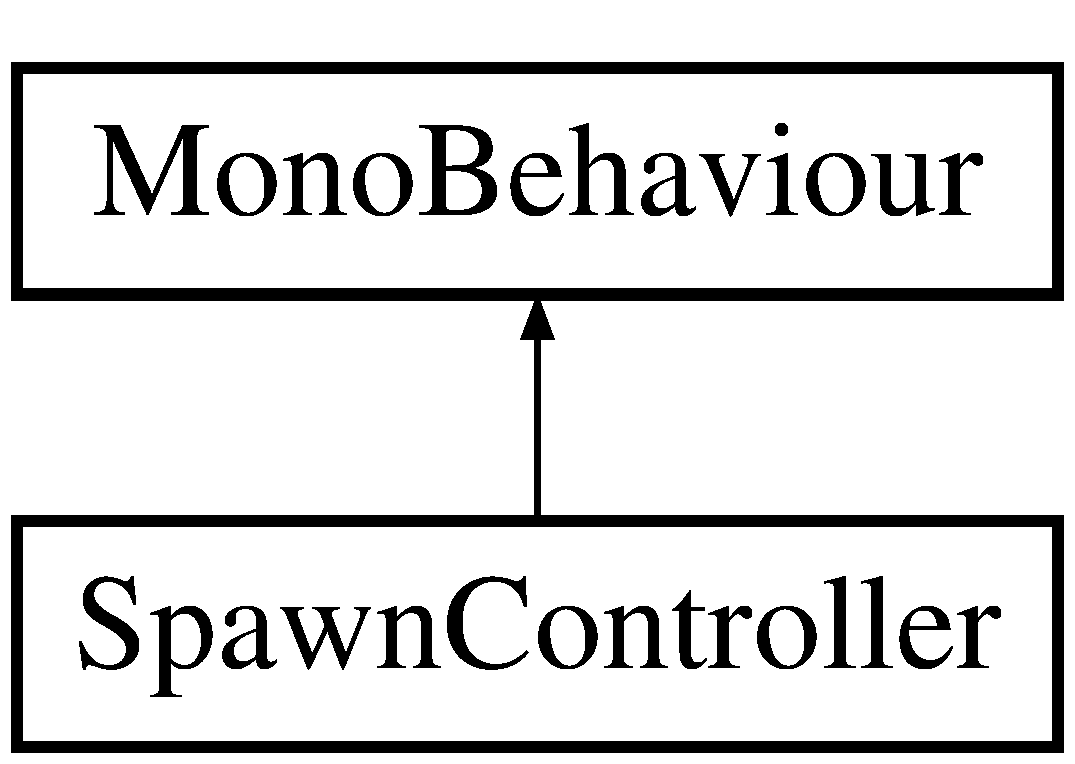
\includegraphics[height=2.000000cm]{class_spawn_controller}
\end{center}
\end{figure}
\subsection*{Public Attributes}
\begin{DoxyCompactItemize}
\item 
\mbox{\Hypertarget{class_spawn_controller_acd9a03f2504ffc0bee3cb51f49ffe70d}\label{class_spawn_controller_acd9a03f2504ffc0bee3cb51f49ffe70d}} 
Game\+Object \hyperlink{class_spawn_controller_acd9a03f2504ffc0bee3cb51f49ffe70d}{enemy}
\begin{DoxyCompactList}\small\item\em Type of enemy to spawn. \end{DoxyCompactList}\item 
\mbox{\Hypertarget{class_spawn_controller_af5d0d5091092b0d6dcee6f670ba96b59}\label{class_spawn_controller_af5d0d5091092b0d6dcee6f670ba96b59}} 
float \hyperlink{class_spawn_controller_af5d0d5091092b0d6dcee6f670ba96b59}{spawn\+Time}
\begin{DoxyCompactList}\small\item\em How often that type of enemy spawns. \end{DoxyCompactList}\item 
\mbox{\Hypertarget{class_spawn_controller_a094ea9629e5c9d39c4262f865ffae644}\label{class_spawn_controller_a094ea9629e5c9d39c4262f865ffae644}} 
Transform \mbox{[}$\,$\mbox{]} \hyperlink{class_spawn_controller_a094ea9629e5c9d39c4262f865ffae644}{spawn\+Points}
\begin{DoxyCompactList}\small\item\em avaible spawnpoints for that type of enemy \end{DoxyCompactList}\end{DoxyCompactItemize}
\subsection*{Private Member Functions}
\begin{DoxyCompactItemize}
\item 
void \hyperlink{class_spawn_controller_a5aa835725a1507e10580c9887069f243}{Start} ()
\item 
void \hyperlink{class_spawn_controller_ac102b761c5d0f090ef09acaeb5180f8b}{Spawn} ()
\end{DoxyCompactItemize}
\subsection*{Private Attributes}
\begin{DoxyCompactItemize}
\item 
\mbox{\Hypertarget{class_spawn_controller_a168d59f6d4b8be8f74aa1bd0c1dd5de3}\label{class_spawn_controller_a168d59f6d4b8be8f74aa1bd0c1dd5de3}} 
float \hyperlink{class_spawn_controller_a168d59f6d4b8be8f74aa1bd0c1dd5de3}{player\+Health}
\begin{DoxyCompactList}\small\item\em Keeps track of current player health. \end{DoxyCompactList}\end{DoxyCompactItemize}


\subsection{Detailed Description}
Handles how a specific enemy mob spawns. \begin{DoxyNote}{Note}
Prefab class 
\end{DoxyNote}


\subsection{Member Function Documentation}
\mbox{\Hypertarget{class_spawn_controller_ac102b761c5d0f090ef09acaeb5180f8b}\label{class_spawn_controller_ac102b761c5d0f090ef09acaeb5180f8b}} 
\index{Spawn\+Controller@{Spawn\+Controller}!Spawn@{Spawn}}
\index{Spawn@{Spawn}!Spawn\+Controller@{Spawn\+Controller}}
\subsubsection{\texorpdfstring{Spawn()}{Spawn()}}
{\footnotesize\ttfamily void Spawn\+Controller.\+Spawn (\begin{DoxyParamCaption}{ }\end{DoxyParamCaption})\hspace{0.3cm}{\ttfamily [private]}}

Spawns a new mob if the player is not dead \mbox{\Hypertarget{class_spawn_controller_a5aa835725a1507e10580c9887069f243}\label{class_spawn_controller_a5aa835725a1507e10580c9887069f243}} 
\index{Spawn\+Controller@{Spawn\+Controller}!Start@{Start}}
\index{Start@{Start}!Spawn\+Controller@{Spawn\+Controller}}
\subsubsection{\texorpdfstring{Start()}{Start()}}
{\footnotesize\ttfamily void Spawn\+Controller.\+Start (\begin{DoxyParamCaption}{ }\end{DoxyParamCaption})\hspace{0.3cm}{\ttfamily [private]}}

Instantiates the \hyperlink{class_spawn_controller}{Spawn\+Controller}
\begin{DoxyItemize}
\item Sets spawntime too 3.\+0f seconds by default
\item Sets Playerhealth
\item and starts the spawn sequence 
\end{DoxyItemize}

The documentation for this class was generated from the following file\+:\begin{DoxyCompactItemize}
\item 
Assets/\+Scripts/\+Controllers/Spawn\+Controller.\+cs\end{DoxyCompactItemize}

\hypertarget{class_spawn_pickups}{}\section{Spawn\+Pickups Class Reference}
\label{class_spawn_pickups}\index{Spawn\+Pickups@{Spawn\+Pickups}}
Inheritance diagram for Spawn\+Pickups\+:\begin{figure}[H]
\begin{center}
\leavevmode
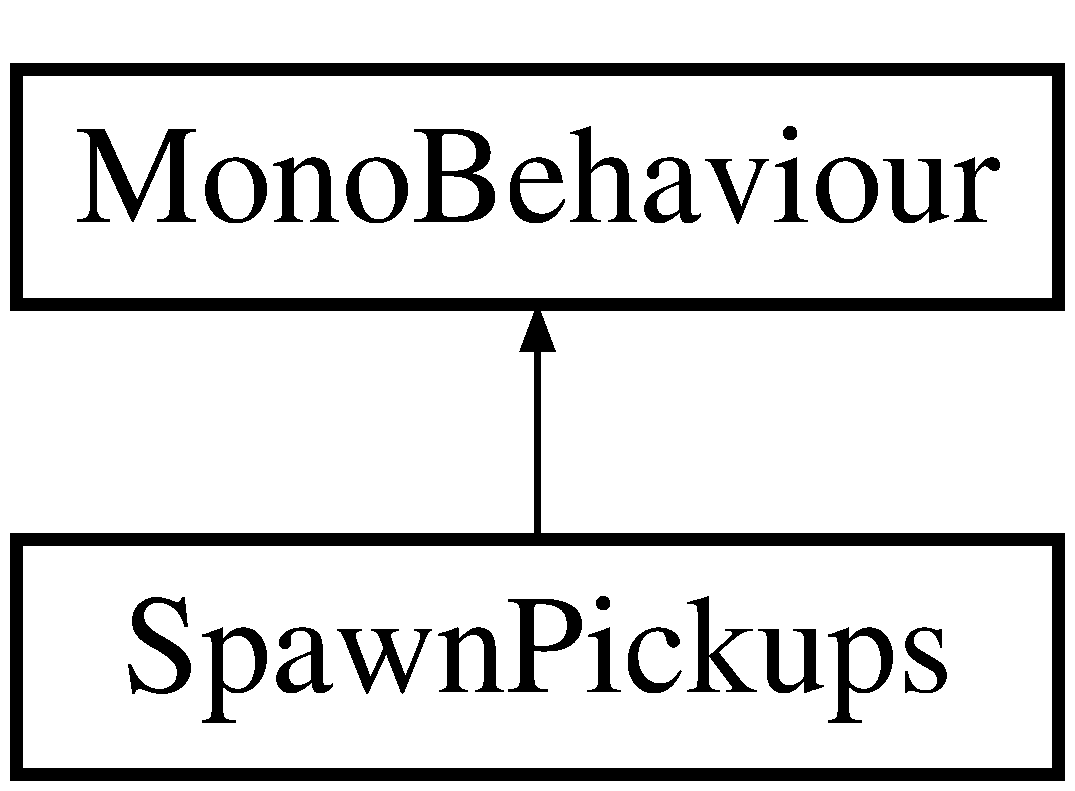
\includegraphics[height=2.000000cm]{class_spawn_pickups}
\end{center}
\end{figure}
\subsection*{Public Attributes}
\begin{DoxyCompactItemize}
\item 
\mbox{\Hypertarget{class_spawn_pickups_a2784fda860bf537ba9c2c798a9454146}\label{class_spawn_pickups_a2784fda860bf537ba9c2c798a9454146}} 
float {\bfseries radius} = 20.\+0f
\item 
\mbox{\Hypertarget{class_spawn_pickups_aef77ed42b74aa4ebd643dac1bb3119e1}\label{class_spawn_pickups_aef77ed42b74aa4ebd643dac1bb3119e1}} 
List$<$ \hyperlink{class_pickup}{Pickup} $>$ {\bfseries Prefab\+List} = new List$<$\hyperlink{class_pickup}{Pickup}$>$()
\end{DoxyCompactItemize}
\subsection*{Private Member Functions}
\begin{DoxyCompactItemize}
\item 
\mbox{\Hypertarget{class_spawn_pickups_a964eeb8fdc5f9158be949895c16fa9c7}\label{class_spawn_pickups_a964eeb8fdc5f9158be949895c16fa9c7}} 
void {\bfseries Update} ()
\end{DoxyCompactItemize}
\subsection*{Private Attributes}
\begin{DoxyCompactItemize}
\item 
\mbox{\Hypertarget{class_spawn_pickups_a20980cde8781cd088722db7ebdb1ce6d}\label{class_spawn_pickups_a20980cde8781cd088722db7ebdb1ce6d}} 
float {\bfseries timer} = 0.\+0f
\end{DoxyCompactItemize}


\subsection{Detailed Description}
Spawns certain items 

The documentation for this class was generated from the following file\+:\begin{DoxyCompactItemize}
\item 
Assets/\+Scripts/\+Entities/Spawn\+Pickups.\+cs\end{DoxyCompactItemize}

\hypertarget{class_spell}{}\section{Spell Class Reference}
\label{class_spell}\index{Spell@{Spell}}
\subsection*{Public Member Functions}
\begin{DoxyCompactItemize}
\item 
\mbox{\Hypertarget{class_spell_a69429a1783933ad446ee57e9a35b10de}\label{class_spell_a69429a1783933ad446ee57e9a35b10de}} 
{\bfseries Spell} (bool un, double dm, string na, float sm)
\end{DoxyCompactItemize}
\subsection*{Public Attributes}
\begin{DoxyCompactItemize}
\item 
\mbox{\Hypertarget{class_spell_aafd49e25b1309ecfc23b56e1aaabfd19}\label{class_spell_aafd49e25b1309ecfc23b56e1aaabfd19}} 
bool {\bfseries unlocked}
\item 
\mbox{\Hypertarget{class_spell_a79d53f2fffa4b3ad9e4adb166430a9fc}\label{class_spell_a79d53f2fffa4b3ad9e4adb166430a9fc}} 
double {\bfseries dmg\+Mult}
\item 
\mbox{\Hypertarget{class_spell_ae6a6af372417cf9f204db6ea1cb18de6}\label{class_spell_ae6a6af372417cf9f204db6ea1cb18de6}} 
string {\bfseries name}
\item 
\mbox{\Hypertarget{class_spell_ab0a70c8037e539a887c0447d5f5d72e2}\label{class_spell_ab0a70c8037e539a887c0447d5f5d72e2}} 
float {\bfseries speed\+Mult}
\end{DoxyCompactItemize}


The documentation for this class was generated from the following file\+:\begin{DoxyCompactItemize}
\item 
Assets/\+Scripts/\+Arrows/Spell.\+cs\end{DoxyCompactItemize}

\hypertarget{class_spell_controller}{}\section{Spell\+Controller Class Reference}
\label{class_spell_controller}\index{Spell\+Controller@{Spell\+Controller}}
Inheritance diagram for Spell\+Controller\+:\begin{figure}[H]
\begin{center}
\leavevmode
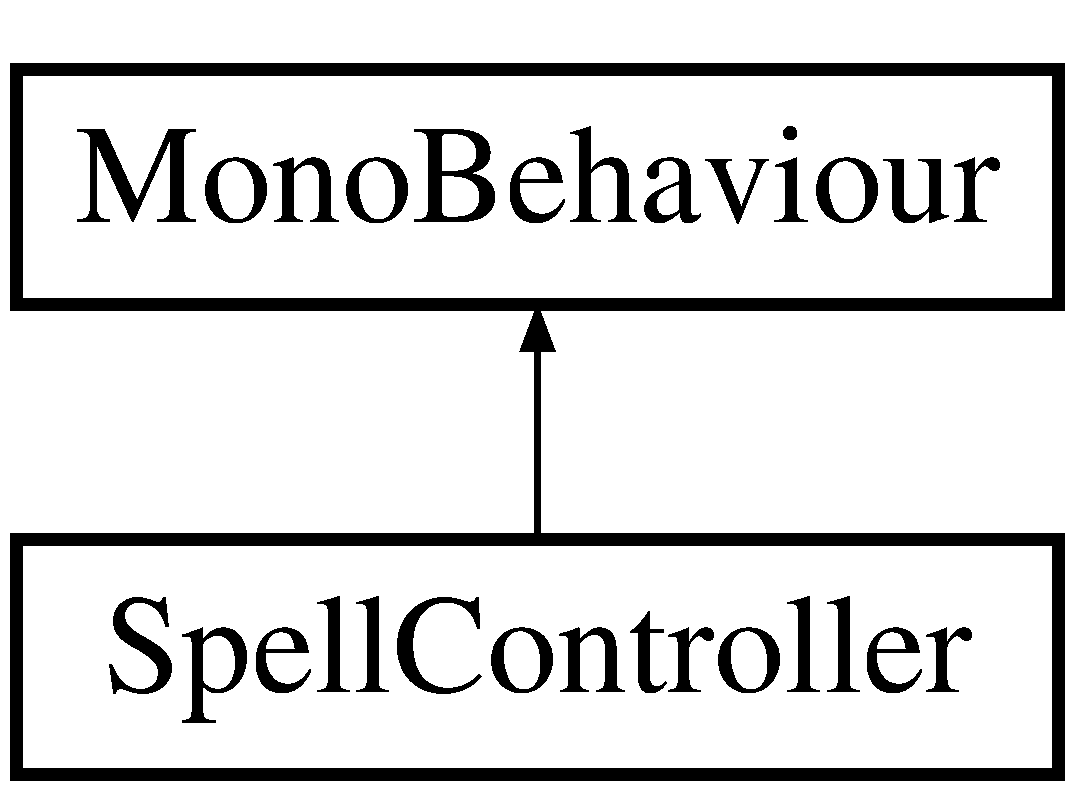
\includegraphics[height=2.000000cm]{class_spell_controller}
\end{center}
\end{figure}
\subsection*{Public Member Functions}
\begin{DoxyCompactItemize}
\item 
void \hyperlink{class_spell_controller_a63da1ad10f9cb7931912cd60704875f5}{Start} ()
\item 
void \hyperlink{class_spell_controller_a21bc9cc1d9dcf0fdebc52754a9008552}{Update} ()
\item 
void \hyperlink{class_spell_controller_a779832e1b2aa56a36708f5fe7c7cc434}{Spawn\+Arrow} (Game\+Object arrow)
\item 
void \hyperlink{class_spell_controller_a60e9f69e1644149911c54e667a297ba8}{Start\+Spawn\+Sequence} ()
\item 
void \hyperlink{class_spell_controller_a9b3f29e4230fcdf1b601c6a8d49574e0}{End\+Spawn\+Sequence} ()
\item 
float \hyperlink{class_spell_controller_ad6e891fc9dd19a3eccec2a05791abff4}{Get\+Osu\+Time} ()
\end{DoxyCompactItemize}
\subsection*{Public Attributes}
\begin{DoxyCompactItemize}
\item 
\mbox{\Hypertarget{class_spell_controller_a70254f75318edd987407835df7806046}\label{class_spell_controller_a70254f75318edd987407835df7806046}} 
Game\+Object {\bfseries basic\+Arrow}
\item 
Game\+Object \hyperlink{class_spell_controller_aa36968ec27a32acb26ec87db86af9415}{Fast\+Arrow}
\begin{DoxyCompactList}\small\item\em Basic arrow to be instantiated on load. \end{DoxyCompactList}\item 
\mbox{\Hypertarget{class_spell_controller_a2d0099eccd4c793b1a97ad6bde7a0733}\label{class_spell_controller_a2d0099eccd4c793b1a97ad6bde7a0733}} 
bool \hyperlink{class_spell_controller_a2d0099eccd4c793b1a97ad6bde7a0733}{firing}
\begin{DoxyCompactList}\small\item\em boolean to keep track of player state \end{DoxyCompactList}\item 
\mbox{\Hypertarget{class_spell_controller_a6d3ca0bdc911a31cf5036441339b075c}\label{class_spell_controller_a6d3ca0bdc911a31cf5036441339b075c}} 
float \hyperlink{class_spell_controller_a6d3ca0bdc911a31cf5036441339b075c}{osu\+Time\+Scale}
\begin{DoxyCompactList}\small\item\em speed of the Osu\+Circles \end{DoxyCompactList}\item 
\mbox{\Hypertarget{class_spell_controller_a16ce771d6fc67978547d50e604d8e3d9}\label{class_spell_controller_a16ce771d6fc67978547d50e604d8e3d9}} 
Game\+Object \hyperlink{class_spell_controller_a16ce771d6fc67978547d50e604d8e3d9}{loaded}
\begin{DoxyCompactList}\small\item\em default arrow that gets interchanged on osucircle selection \end{DoxyCompactList}\end{DoxyCompactItemize}
\subsection*{Private Attributes}
\begin{DoxyCompactItemize}
\item 
\mbox{\Hypertarget{class_spell_controller_a01fd503ede5facdd5e8dd6ed02dca4ba}\label{class_spell_controller_a01fd503ede5facdd5e8dd6ed02dca4ba}} 
\hyperlink{class_u_i_controller}{U\+I\+Controller} \hyperlink{class_spell_controller_a01fd503ede5facdd5e8dd6ed02dca4ba}{U\+I\+Controller}
\begin{DoxyCompactList}\small\item\em \hyperlink{class_u_i_controller}{U\+I\+Controller} object for communication. \end{DoxyCompactList}\item 
\mbox{\Hypertarget{class_spell_controller_aebf669b2371dc1e055144a731ad56a84}\label{class_spell_controller_aebf669b2371dc1e055144a731ad56a84}} 
\hyperlink{class_game_controller}{Game\+Controller} \hyperlink{class_spell_controller_aebf669b2371dc1e055144a731ad56a84}{Game\+Controller}
\begin{DoxyCompactList}\small\item\em \hyperlink{class_game_controller}{Game\+Controller} object for communication. \end{DoxyCompactList}\item 
\mbox{\Hypertarget{class_spell_controller_a29b551a129180a586d25625380f6eb39}\label{class_spell_controller_a29b551a129180a586d25625380f6eb39}} 
Game\+Object \hyperlink{class_spell_controller_a29b551a129180a586d25625380f6eb39}{player}
\begin{DoxyCompactList}\small\item\em \hyperlink{class_player}{Player} object. \end{DoxyCompactList}\item 
\mbox{\Hypertarget{class_spell_controller_a7448d6b3424043cb1b182e82d0008a6d}\label{class_spell_controller_a7448d6b3424043cb1b182e82d0008a6d}} 
float \hyperlink{class_spell_controller_a7448d6b3424043cb1b182e82d0008a6d}{osu\+Time}
\begin{DoxyCompactList}\small\item\em variable to keep track of how close the user was to clicking the circle in time \end{DoxyCompactList}\end{DoxyCompactItemize}


\subsection{Detailed Description}
Handles spell interactions in the game 

\subsection{Member Function Documentation}
\mbox{\Hypertarget{class_spell_controller_a9b3f29e4230fcdf1b601c6a8d49574e0}\label{class_spell_controller_a9b3f29e4230fcdf1b601c6a8d49574e0}} 
\index{Spell\+Controller@{Spell\+Controller}!End\+Spawn\+Sequence@{End\+Spawn\+Sequence}}
\index{End\+Spawn\+Sequence@{End\+Spawn\+Sequence}!Spell\+Controller@{Spell\+Controller}}
\subsubsection{\texorpdfstring{End\+Spawn\+Sequence()}{EndSpawnSequence()}}
{\footnotesize\ttfamily void Spell\+Controller.\+End\+Spawn\+Sequence (\begin{DoxyParamCaption}{ }\end{DoxyParamCaption})}

Instantiates the loaded arrow upon bow release \mbox{\Hypertarget{class_spell_controller_ad6e891fc9dd19a3eccec2a05791abff4}\label{class_spell_controller_ad6e891fc9dd19a3eccec2a05791abff4}} 
\index{Spell\+Controller@{Spell\+Controller}!Get\+Osu\+Time@{Get\+Osu\+Time}}
\index{Get\+Osu\+Time@{Get\+Osu\+Time}!Spell\+Controller@{Spell\+Controller}}
\subsubsection{\texorpdfstring{Get\+Osu\+Time()}{GetOsuTime()}}
{\footnotesize\ttfamily float Spell\+Controller.\+Get\+Osu\+Time (\begin{DoxyParamCaption}{ }\end{DoxyParamCaption})}

returns a float (seconds) on how close the player was to hitting the Approach circle in the appropriate time \mbox{\Hypertarget{class_spell_controller_a779832e1b2aa56a36708f5fe7c7cc434}\label{class_spell_controller_a779832e1b2aa56a36708f5fe7c7cc434}} 
\index{Spell\+Controller@{Spell\+Controller}!Spawn\+Arrow@{Spawn\+Arrow}}
\index{Spawn\+Arrow@{Spawn\+Arrow}!Spell\+Controller@{Spell\+Controller}}
\subsubsection{\texorpdfstring{Spawn\+Arrow()}{SpawnArrow()}}
{\footnotesize\ttfamily void Spell\+Controller.\+Spawn\+Arrow (\begin{DoxyParamCaption}\item[{Game\+Object}]{arrow }\end{DoxyParamCaption})}


\begin{DoxyParams}{Parameters}
{\em instantiates} & an arrow gameobject \\
\hline
\end{DoxyParams}
\mbox{\Hypertarget{class_spell_controller_a63da1ad10f9cb7931912cd60704875f5}\label{class_spell_controller_a63da1ad10f9cb7931912cd60704875f5}} 
\index{Spell\+Controller@{Spell\+Controller}!Start@{Start}}
\index{Start@{Start}!Spell\+Controller@{Spell\+Controller}}
\subsubsection{\texorpdfstring{Start()}{Start()}}
{\footnotesize\ttfamily void Spell\+Controller.\+Start (\begin{DoxyParamCaption}{ }\end{DoxyParamCaption})}

Sets member values \mbox{\Hypertarget{class_spell_controller_a60e9f69e1644149911c54e667a297ba8}\label{class_spell_controller_a60e9f69e1644149911c54e667a297ba8}} 
\index{Spell\+Controller@{Spell\+Controller}!Start\+Spawn\+Sequence@{Start\+Spawn\+Sequence}}
\index{Start\+Spawn\+Sequence@{Start\+Spawn\+Sequence}!Spell\+Controller@{Spell\+Controller}}
\subsubsection{\texorpdfstring{Start\+Spawn\+Sequence()}{StartSpawnSequence()}}
{\footnotesize\ttfamily void Spell\+Controller.\+Start\+Spawn\+Sequence (\begin{DoxyParamCaption}{ }\end{DoxyParamCaption})}

Starts the arrow shooting sequence. Sets loaded arrow to default basic\+Arrow. Loaded then changes based on whether or not an Osucircle had been clicked. \mbox{\Hypertarget{class_spell_controller_a21bc9cc1d9dcf0fdebc52754a9008552}\label{class_spell_controller_a21bc9cc1d9dcf0fdebc52754a9008552}} 
\index{Spell\+Controller@{Spell\+Controller}!Update@{Update}}
\index{Update@{Update}!Spell\+Controller@{Spell\+Controller}}
\subsubsection{\texorpdfstring{Update()}{Update()}}
{\footnotesize\ttfamily void Spell\+Controller.\+Update (\begin{DoxyParamCaption}{ }\end{DoxyParamCaption})}

Update checks gamestates in current frame for any updates to spell related events, such as new arrows or firing/ 

\subsection{Member Data Documentation}
\mbox{\Hypertarget{class_spell_controller_aa36968ec27a32acb26ec87db86af9415}\label{class_spell_controller_aa36968ec27a32acb26ec87db86af9415}} 
\index{Spell\+Controller@{Spell\+Controller}!Fast\+Arrow@{Fast\+Arrow}}
\index{Fast\+Arrow@{Fast\+Arrow}!Spell\+Controller@{Spell\+Controller}}
\subsubsection{\texorpdfstring{Fast\+Arrow}{FastArrow}}
{\footnotesize\ttfamily Game\+Object Spell\+Controller.\+Fast\+Arrow}



Basic arrow to be instantiated on load. 

fastarrow to be instantiated on osucircle click 

The documentation for this class was generated from the following file\+:\begin{DoxyCompactItemize}
\item 
Assets/\+Scripts/\+Controllers/Spell\+Controller.\+cs\end{DoxyCompactItemize}

\hypertarget{class_u_i_controller}{}\section{U\+I\+Controller Class Reference}
\label{class_u_i_controller}\index{U\+I\+Controller@{U\+I\+Controller}}
Inheritance diagram for U\+I\+Controller\+:\begin{figure}[H]
\begin{center}
\leavevmode
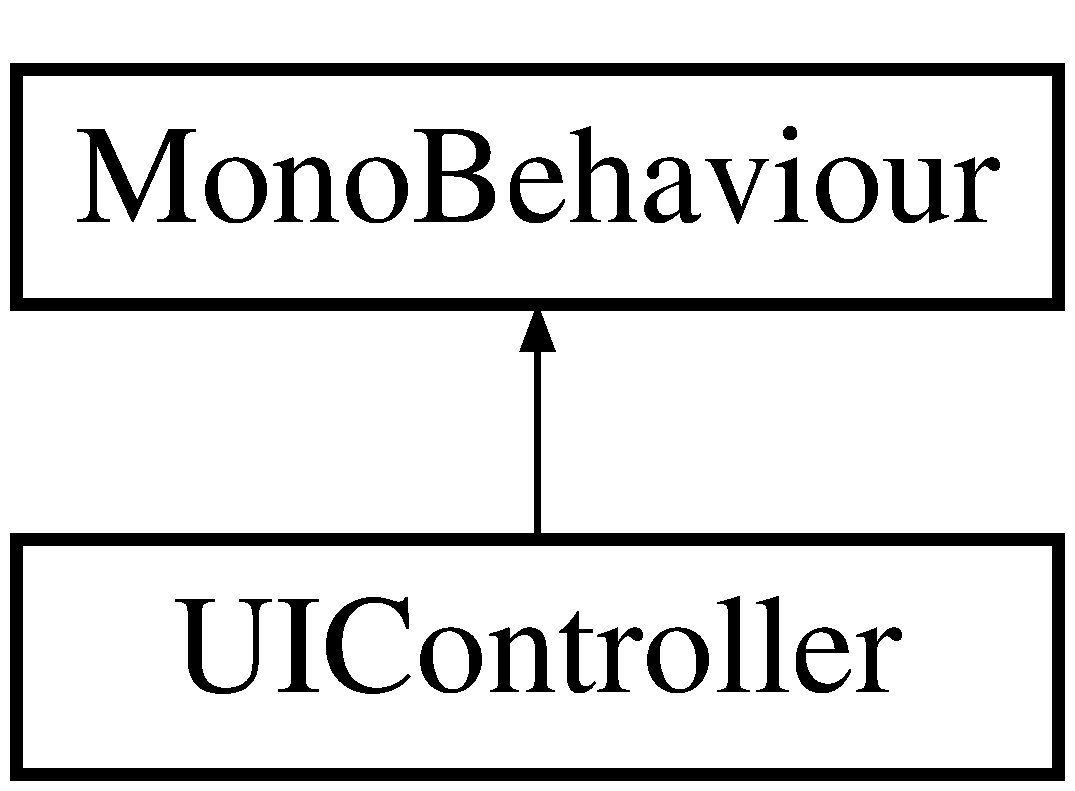
\includegraphics[height=2.000000cm]{class_u_i_controller}
\end{center}
\end{figure}
\subsection*{Public Member Functions}
\begin{DoxyCompactItemize}
\item 
void \hyperlink{class_u_i_controller_a87a0993fd494e90a55c6414d75467dd7}{Update\+Score} (int num)
\item 
int \hyperlink{class_u_i_controller_a4d9cf4f88502ba97bf5b1956ba24773d}{Get\+Score} ()
\item 
void \hyperlink{class_u_i_controller_a0c9a9ed0d8276bed8374ee2ee484ff0f}{Show\+Game\+Over} ()
\item 
void \hyperlink{class_u_i_controller_a96b6e594843a18425eddbb2adc5ede02}{Shooting} ()
\item 
void \hyperlink{class_u_i_controller_a720867c07d063e353bd105d582ad3646}{Release} ()
\end{DoxyCompactItemize}
\subsection*{Public Attributes}
\begin{DoxyCompactItemize}
\item 
\mbox{\Hypertarget{class_u_i_controller_aac6233fbba2e67548334fcebda846b13}\label{class_u_i_controller_aac6233fbba2e67548334fcebda846b13}} 
Texture2D \hyperlink{class_u_i_controller_aac6233fbba2e67548334fcebda846b13}{cursor\+Texture}
\begin{DoxyCompactList}\small\item\em Custom Cursor textures changed in the Editor. \end{DoxyCompactList}\item 
\mbox{\Hypertarget{class_u_i_controller_a06c89b8bab048dc7da9e95f83dc98512}\label{class_u_i_controller_a06c89b8bab048dc7da9e95f83dc98512}} 
Game\+Object \hyperlink{class_u_i_controller_a06c89b8bab048dc7da9e95f83dc98512}{Aim\+Line}
\begin{DoxyCompactList}\small\item\em Gameobject that handles aim line. \end{DoxyCompactList}\item 
\mbox{\Hypertarget{class_u_i_controller_a21bbf8d28555e4bbbf02eb36b3b4fd09}\label{class_u_i_controller_a21bbf8d28555e4bbbf02eb36b3b4fd09}} 
Game\+Object \hyperlink{class_u_i_controller_a21bbf8d28555e4bbbf02eb36b3b4fd09}{Shooting\+Aim\+Line}
\begin{DoxyCompactList}\small\item\em Gameobject that handles the growing line. \end{DoxyCompactList}\item 
\mbox{\Hypertarget{class_u_i_controller_a6ea44aea6d6acc117d660b518612e983}\label{class_u_i_controller_a6ea44aea6d6acc117d660b518612e983}} 
bool \hyperlink{class_u_i_controller_a6ea44aea6d6acc117d660b518612e983}{is\+Shooting}
\begin{DoxyCompactList}\small\item\em Boolean object used in shootingaimline. \end{DoxyCompactList}\item 
\mbox{\Hypertarget{class_u_i_controller_a9e07150f7246ddee7be0b4d07040a33d}\label{class_u_i_controller_a9e07150f7246ddee7be0b4d07040a33d}} 
List$<$ Game\+Object $>$ \hyperlink{class_u_i_controller_a9e07150f7246ddee7be0b4d07040a33d}{circle\+Types}
\begin{DoxyCompactList}\small\item\em List of Osu\+Circles that spawn around the player when firing. \end{DoxyCompactList}\item 
\mbox{\Hypertarget{class_u_i_controller_a151e5f189914d2ed009b093e9d6be436}\label{class_u_i_controller_a151e5f189914d2ed009b093e9d6be436}} 
bool \hyperlink{class_u_i_controller_a151e5f189914d2ed009b093e9d6be436}{is\+Game\+Over} = false
\begin{DoxyCompactList}\small\item\em Managed in scenes and menus (death menu) \end{DoxyCompactList}\item 
\mbox{\Hypertarget{class_u_i_controller_a3de0644d27645eb1981abc610a3a82f9}\label{class_u_i_controller_a3de0644d27645eb1981abc610a3a82f9}} 
Canvas \hyperlink{class_u_i_controller_a3de0644d27645eb1981abc610a3a82f9}{game\+Over}
\begin{DoxyCompactList}\small\item\em Death menu canvas. \end{DoxyCompactList}\item 
\mbox{\Hypertarget{class_u_i_controller_a7d3370f23eac3cedd37d8c9762aaa520}\label{class_u_i_controller_a7d3370f23eac3cedd37d8c9762aaa520}} 
Text \hyperlink{class_u_i_controller_a7d3370f23eac3cedd37d8c9762aaa520}{game\+Over\+Score}
\begin{DoxyCompactList}\small\item\em Death menu Text object. \end{DoxyCompactList}\item 
\mbox{\Hypertarget{class_u_i_controller_a62aa99b5e6e950e1077480846bad3b86}\label{class_u_i_controller_a62aa99b5e6e950e1077480846bad3b86}} 
Text \hyperlink{class_u_i_controller_a62aa99b5e6e950e1077480846bad3b86}{game\+Over\+High\+Score}
\begin{DoxyCompactList}\small\item\em Death menu Highscore text. \end{DoxyCompactList}\item 
\mbox{\Hypertarget{class_u_i_controller_acfe28763f2de32925f0883a3d38792b6}\label{class_u_i_controller_acfe28763f2de32925f0883a3d38792b6}} 
bool \hyperlink{class_u_i_controller_acfe28763f2de32925f0883a3d38792b6}{is\+Pause} = false
\begin{DoxyCompactList}\small\item\em boolean handles pausing and pause canvas \end{DoxyCompactList}\item 
\mbox{\Hypertarget{class_u_i_controller_a3a17542c374d9d162acc7d636d2cdcb9}\label{class_u_i_controller_a3a17542c374d9d162acc7d636d2cdcb9}} 
Game\+Object \hyperlink{class_u_i_controller_a3a17542c374d9d162acc7d636d2cdcb9}{Osu\+Circle}
\begin{DoxyCompactList}\small\item\em Instantiate blank \hyperlink{class_osu_circle}{Osu\+Circle} gameobject. \end{DoxyCompactList}\end{DoxyCompactItemize}
\subsection*{Private Member Functions}
\begin{DoxyCompactItemize}
\item 
void \hyperlink{class_u_i_controller_a676b3b972c33885db4565ee43f23e459}{Start} ()
\end{DoxyCompactItemize}
\subsection*{Private Attributes}
\begin{DoxyCompactItemize}
\item 
\mbox{\Hypertarget{class_u_i_controller_a98e6ab376e28858f95189dbdbda70620}\label{class_u_i_controller_a98e6ab376e28858f95189dbdbda70620}} 
Game\+Object \hyperlink{class_u_i_controller_a98e6ab376e28858f95189dbdbda70620}{player}
\begin{DoxyCompactList}\small\item\em \hyperlink{class_player}{Player} object. \end{DoxyCompactList}\item 
\mbox{\Hypertarget{class_u_i_controller_a2dabfeddc98455ff4a93d843ebb6c4d8}\label{class_u_i_controller_a2dabfeddc98455ff4a93d843ebb6c4d8}} 
Vector2 \hyperlink{class_u_i_controller_a2dabfeddc98455ff4a93d843ebb6c4d8}{hot\+Spot} = Vector2.\+zero
\begin{DoxyCompactList}\small\item\em Offset of the cursor (based on where anchor is set) \end{DoxyCompactList}\item 
\mbox{\Hypertarget{class_u_i_controller_a5f32d4a4d789be31b0bd9609ff2307a2}\label{class_u_i_controller_a5f32d4a4d789be31b0bd9609ff2307a2}} 
Game\+Object \hyperlink{class_u_i_controller_a5f32d4a4d789be31b0bd9609ff2307a2}{shootline}
\begin{DoxyCompactList}\small\item\em private gameobject \end{DoxyCompactList}\item 
\mbox{\Hypertarget{class_u_i_controller_a9eb845eb67cb3403b17de6bd505a4379}\label{class_u_i_controller_a9eb845eb67cb3403b17de6bd505a4379}} 
Text \hyperlink{class_u_i_controller_a9eb845eb67cb3403b17de6bd505a4379}{score\+Text}
\begin{DoxyCompactList}\small\item\em Score. \end{DoxyCompactList}\item 
\mbox{\Hypertarget{class_u_i_controller_a8cca6d3f1aee858d74eef5bd8f1846d2}\label{class_u_i_controller_a8cca6d3f1aee858d74eef5bd8f1846d2}} 
int \hyperlink{class_u_i_controller_a8cca6d3f1aee858d74eef5bd8f1846d2}{score}
\begin{DoxyCompactList}\small\item\em current Int value of score \end{DoxyCompactList}\end{DoxyCompactItemize}


\subsection{Detailed Description}
Controller object that handles most UI interactions in the Game\+Scene 

\subsection{Member Function Documentation}
\mbox{\Hypertarget{class_u_i_controller_a4d9cf4f88502ba97bf5b1956ba24773d}\label{class_u_i_controller_a4d9cf4f88502ba97bf5b1956ba24773d}} 
\index{U\+I\+Controller@{U\+I\+Controller}!Get\+Score@{Get\+Score}}
\index{Get\+Score@{Get\+Score}!U\+I\+Controller@{U\+I\+Controller}}
\subsubsection{\texorpdfstring{Get\+Score()}{GetScore()}}
{\footnotesize\ttfamily int U\+I\+Controller.\+Get\+Score (\begin{DoxyParamCaption}{ }\end{DoxyParamCaption})}

Returns score \mbox{\Hypertarget{class_u_i_controller_a720867c07d063e353bd105d582ad3646}\label{class_u_i_controller_a720867c07d063e353bd105d582ad3646}} 
\index{U\+I\+Controller@{U\+I\+Controller}!Release@{Release}}
\index{Release@{Release}!U\+I\+Controller@{U\+I\+Controller}}
\subsubsection{\texorpdfstring{Release()}{Release()}}
{\footnotesize\ttfamily void U\+I\+Controller.\+Release (\begin{DoxyParamCaption}{ }\end{DoxyParamCaption})}

UI Elements on shooting Release \mbox{\Hypertarget{class_u_i_controller_a96b6e594843a18425eddbb2adc5ede02}\label{class_u_i_controller_a96b6e594843a18425eddbb2adc5ede02}} 
\index{U\+I\+Controller@{U\+I\+Controller}!Shooting@{Shooting}}
\index{Shooting@{Shooting}!U\+I\+Controller@{U\+I\+Controller}}
\subsubsection{\texorpdfstring{Shooting()}{Shooting()}}
{\footnotesize\ttfamily void U\+I\+Controller.\+Shooting (\begin{DoxyParamCaption}{ }\end{DoxyParamCaption})}

Instantiates Shooting UI elements (Like Osu Circles) reads in list of Circle\+Types (prefabs) \mbox{\Hypertarget{class_u_i_controller_a0c9a9ed0d8276bed8374ee2ee484ff0f}\label{class_u_i_controller_a0c9a9ed0d8276bed8374ee2ee484ff0f}} 
\index{U\+I\+Controller@{U\+I\+Controller}!Show\+Game\+Over@{Show\+Game\+Over}}
\index{Show\+Game\+Over@{Show\+Game\+Over}!U\+I\+Controller@{U\+I\+Controller}}
\subsubsection{\texorpdfstring{Show\+Game\+Over()}{ShowGameOver()}}
{\footnotesize\ttfamily void U\+I\+Controller.\+Show\+Game\+Over (\begin{DoxyParamCaption}{ }\end{DoxyParamCaption})}

Creates the Game\+Over menu \mbox{\Hypertarget{class_u_i_controller_a676b3b972c33885db4565ee43f23e459}\label{class_u_i_controller_a676b3b972c33885db4565ee43f23e459}} 
\index{U\+I\+Controller@{U\+I\+Controller}!Start@{Start}}
\index{Start@{Start}!U\+I\+Controller@{U\+I\+Controller}}
\subsubsection{\texorpdfstring{Start()}{Start()}}
{\footnotesize\ttfamily void U\+I\+Controller.\+Start (\begin{DoxyParamCaption}{ }\end{DoxyParamCaption})\hspace{0.3cm}{\ttfamily [private]}}

Instantiates all members and UI Assets Also sets default values for scoores and Canvases \mbox{\Hypertarget{class_u_i_controller_a87a0993fd494e90a55c6414d75467dd7}\label{class_u_i_controller_a87a0993fd494e90a55c6414d75467dd7}} 
\index{U\+I\+Controller@{U\+I\+Controller}!Update\+Score@{Update\+Score}}
\index{Update\+Score@{Update\+Score}!U\+I\+Controller@{U\+I\+Controller}}
\subsubsection{\texorpdfstring{Update\+Score()}{UpdateScore()}}
{\footnotesize\ttfamily void U\+I\+Controller.\+Update\+Score (\begin{DoxyParamCaption}\item[{int}]{num }\end{DoxyParamCaption})}

Updates score shown on canvas 
\begin{DoxyParams}{Parameters}
{\em num} & is the score that needs to be updated \\
\hline
\end{DoxyParams}


The documentation for this class was generated from the following file\+:\begin{DoxyCompactItemize}
\item 
Assets/\+Scripts/\+Controllers/U\+I\+Controller.\+cs\end{DoxyCompactItemize}

%--- End generated contents ---

% Index
\backmatter
\newpage
\phantomsection
\clearemptydoublepage
\addcontentsline{toc}{chapter}{Index}
\printindex

\end{document}
